% =====================================================================
%  main.tex — 主文件（Lead 独占）
%  编译：在 源码\ 目录下 `xelatex main.tex` 两遍（或 ..\工程文件\build.ps1）
% =====================================================================
\documentclass[UTF8,a4paper,11pt]{ctexart}
% =====================================================================
%  preamble.tex  —  导言区（SY03-22 Dan Xie《General Argyres-Douglas Theory》中文译注本）
%  由 Lead 维护；译者只读。缺宏时在文末「追加区」append \newcommand，
%  并在回报里列出新增宏名（不得改动上面的已有定义）。
% =====================================================================
\usepackage[a4paper,margin=2.6cm,top=3.0cm,bottom=2.8cm]{geometry}
\usepackage{amsmath,amssymb,amsthm,mathtools}
\usepackage{mathrsfs}
\usepackage{graphicx}
\usepackage{tikz}
\usetikzlibrary{calc,positioning,decorations.pathmorphing,decorations.markings,patterns,arrows}
\usepackage{array,booktabs,longtable,multirow}
\usepackage{caption}
\usepackage{enumitem}
\usepackage{xcolor}
\usepackage{fancyhdr}

% ---------- 字体（Windows，显式路径） ----------
\setCJKmainfont[Path=C:/Windows/Fonts/,BoldFont=simhei.ttf,ItalicFont=simkai.ttf]{simsun.ttc}
\setCJKsansfont[Path=C:/Windows/Fonts/]{simhei.ttf}
\setCJKmonofont[Path=C:/Windows/Fonts/]{simfang.ttf}
\setCJKfamilyfont{zhkai}[Path=C:/Windows/Fonts/]{simkai.ttf}
\setCJKfamilyfont{zhhei}[Path=C:/Windows/Fonts/]{simhei.ttf}
\setCJKfamilyfont{zhfang}[Path=C:/Windows/Fonts/]{simfang.ttf}
\providecommand{\kaishu}{\CJKfamily{zhkai}}
\providecommand{\heiti}{\CJKfamily{zhhei}}
\providecommand{\fangsong}{\CJKfamily{zhfang}}

% ---------- 数学宏（块文件里只许用这些，禁止自造） ----------
\newcommand{\sN}{\mathcal{N}}          % 超对称数 \sN=2
\newcommand{\sA}{\mathcal{A}}          % 平坦联络 𝒜 = A + iφ
\newcommand{\sM}{\mathcal{M}}          % 模空间
\newcommand{\sO}{\mathcal{O}}          % 算子
\newcommand{\sD}{\mathcal{D}}          % 判别式
\DeclareMathOperator{\Tr}{Tr}
\DeclareMathOperator{\diag}{diag}
\DeclareMathOperator{\SU}{SU}
\DeclareMathOperator{\SO}{SO}
\DeclareMathOperator{\U}{U}
\DeclareMathOperator{\Sl}{Sl}
\DeclareMathOperator{\SlN}{Sl}
\newcommand{\R}{\mathbb{R}}
\newcommand{\C}{\mathbb{C}}
\newcommand{\Z}{\mathbb{Z}}
\newcommand{\Q}{\mathbb{Q}}
\newcommand{\CP}{\mathbb{CP}}
\newcommand{\eps}{\varepsilon}
\newcommand{\dd}{\mathrm{d}}
\newcommand{\ee}{\mathrm{e}}
\newcommand{\ii}{\mathrm{i}}
\newcommand{\half}{\tfrac{1}{2}}
\newcommand{\third}{\tfrac{1}{3}}
\newcommand{\Ncoupling}{N_{\text{coupling}}}
% 表格里常用的列类型
\newcolumntype{C}[1]{>{\centering\arraybackslash}p{#1}}

% ---------- 定理类环境（编号一律手工给：\begin{theorem}[3.1]） ----------
\theoremstyle{definition}
\newtheorem*{theorem}{定理}
\newtheorem*{proposition}{命题}
\newtheorem*{lemma}{引理}
\newtheorem*{corollary}{推论}
\newtheorem*{definition}{定义}
\newtheorem*{example}{例}
\newtheorem*{remark}{注}

% ---------- 译注 / 路线注 ----------
% 译注：解释性补充，必须带 [来源：…]（A/B/I 级）或 [译者按（无外部依据）…]
\newcommand{\zhnote}[1]{\par\smallskip\noindent
  {\small\kaishu\color{black!85}【译注】#1}\par\smallskip}
% 路线注：说明作者的论证路线（为什么先证这个 / 哪条路被放弃），必须带原书页码 p.NN
\newcommand{\routenote}[1]{\par\smallskip\noindent
  {\small\kaishu\color{black!70}【路线】#1}\par\smallskip}
% 原文笔误提示（比译注轻）
\newcommand{\typo}[1]{\par\smallskip\noindent
  {\small\kaishu\color{black!85}【原文如此】#1}\par\smallskip}

% ---------- 版式 ----------
\setlength{\parindent}{2em}
\linespread{1.18}
\setlength{\emergencystretch}{2.5em}
\setlist{nosep,leftmargin=2.2em}
\renewcommand{\arraystretch}{1.15}
\captionsetup{font=small,labelsep=quad}

\pagestyle{fancy}
\fancyhf{}
\fancyhead[L]{\small\kaishu 广义 Argyres--Douglas 理论}
\fancyhead[R]{\small\thepage}
\renewcommand{\headrulewidth}{0.4pt}
\fancypagestyle{plain}{\fancyhf{}\fancyfoot[C]{\small\thepage}\renewcommand{\headrulewidth}{0pt}}

\ctexset{
  section = {
    format = \Large\bfseries\heiti,
    beforeskip = 2.2ex plus 1ex minus .2ex,
    afterskip  = 1.4ex plus .2ex,
    name = {},
    number = \arabic{section},
  },
  subsection = {
    format = \large\bfseries\heiti,
    beforeskip = 1.8ex plus .6ex minus .2ex,
    afterskip  = 1.0ex plus .2ex,
  },
  subsubsection = {
    format = \normalsize\bfseries\heiti,
    beforeskip = 1.4ex plus .5ex minus .2ex,
    afterskip  = 0.8ex plus .2ex,
  },
}

\usepackage[hidelinks,bookmarksnumbered=true,bookmarksopen=true,
            pdftitle={广义 Argyres-Douglas 理论（中文译注本）},
            pdfauthor={Dan Xie}]{hyperref}

% ===================== 追加区（译者可 append \newcommand） =====================


\begin{document}

% ---------------------------- 封面 ----------------------------
\begin{titlepage}
\centering
\vspace*{2.6cm}
{\heiti\zihao{2} 广义 Argyres--Douglas 理论\par}
\vspace{1.0cm}
{\kaishu\zihao{3} General Argyres-Douglas Theory\par}
\vspace{2.0cm}
{\zihao{4} Dan Xie\par}
\vspace{0.5cm}
{\zihao{5} School of Natural Sciences,\\ Institute for Advanced Study, Princeton, NJ 08540\par}
\vspace{1.6cm}
{\kaishu\zihao{4} 中文译注本\par}
\vspace{0.8cm}
{\zihao{5} 底本：arXiv:1204.2270v2 [hep-th]，2016 年 7 月 12 日，54 页（Prepared for submission to JHEP）\par}
\vfill
{\kaishu\zihao{5}
\parbox{0.82\linewidth}{\centering
本译注本依据 arXiv:1204.2270v2 全文翻译：全部 8 节、67 条参考文献、20 幅插图与 4 张表格逐一对应。\\
插图按原文重绘为黑白线稿；原文笔误照译，并以「【原文如此】」或译注指出。}\par}
\vspace{1.0cm}
\end{titlepage}

% ---------------------------- 目录 ----------------------------
{\footnotesize
\tableofcontents}
\newpage

% ------------------------- 译者说明 -------------------------
% =====================================================================
%  translator_note.tex —— 译者说明（放在目录之后、摘要之前）
% =====================================================================
\section*{译者说明}
\addcontentsline{toc}{section}{译者说明}

\textbf{底本。}本书译自 Dan Xie, \emph{General Argyres-Douglas Theory}, arXiv:1204.2270v2 [hep-th]（2016 年 7 月 12 日；Prepared for submission to JHEP），共 54 个印刷页，含插图 20 幅、表格 4 张、参考文献 67 条。文中「p.$N$」一律指底本的印刷页码，与原 PDF 的页序相差 2。

\textbf{版式。}公式编号、图号、表号、文献编号全部照底本原样，不重排、不跳号。插图按底本重绘为黑白线稿，图内标注保留底本写法。行文引用公式时写「式 (n.m)」，不另造编号。

\textbf{术语。}底本使用的术语中，有相当一部分在中文学界没有通行译名，或者通行译名与英文原词的实际所指不符。对这些术语，我们只采用两种处置：一是保留英文原文（例如 abelianization、spray、class S、magical、lamination space），二是在仔细讨论后定出一个中译，并在首次出现处用译注交代其英文与所指。凡属后一种情形，其定案都不是临时决定的。这一领域的核心译名（非正则奇点、正则奇点、穿刺点、极点的阶、牛顿多边形、Stokes 扇区与射线、单值性、Hitchin 纤维化等）沿用本库同一主题既有译本已冻结的译法；尚无定名者，先由两位术语译手各自出提案、逐条互审，再由译者定案并记入工程内的术语表。全部术语的最终写法以该表为准，正文不得另立译名。

\textbf{原文笔误。}底本有若干处笔误与前后不一致（公式中的幂次、分母、下标，图注与正文对不上，符号重号等）。我们的原则是：正文照录原文，不加改动；凡影响理解者，用【原文如此】标出原样，再在译注里给出正确形式与判定依据（通常是由相邻公式反算，或由底本自身的另一处写法互证）。凡属不影响理解的排印瑕疵，径行订正，不出注。

\textbf{译注。}全书有三类标注。

\begin{itemize}
  \item 【译注】：解释性补充。每条都带来源，写作 \verb|[来源：…]| 或 \verb|[依据：…]|，其中来源按 A（底本、作者其他论文、经典教材）、B（nLab、Stacks Project、ProofWiki 等）、I（本库既往译本）三级标注；确实没有外部依据的，写作 \verb|[译者按（无外部依据）：…]|。
  \item 【路线】：交代作者的论证路线——为什么先证这一条、哪条路被放弃、某处结论依赖什么前提。这类注带底本页码。
  \item 【原文如此】：指出底本笔误之处，正文未作改动。
\end{itemize}

\textbf{阅读建议。}第 3 节是技术核心：它给出 Hitchin 方程非正则奇点的分类，后面各节都在用这套分类。只关心物理结果的读者可以跳过第 3.1 节的格点与杨图细节，先读第 4 至 7 节；但第 6.1 节把非正则奇点压成三类的那一步论证（式 (6.6) 处的矛盾）是全篇的枢纽，不宜略过。


% ---------------------------- 摘要 ----------------------------
% =====================================================================
%  abstract.tex —— 摘要（原文 p.1）
% =====================================================================
\begin{center}
{\heiti\large 摘\quad 要}
\end{center}

\noindent
我们用带非正则奇点的黎曼面紧致化六维 $(2,0)$ $A_{N-1}$ 理论，构造了一大类 Argyres--Douglas 型理论。对黎曼面与奇点的选择，我们给出完整的分类。我们算出 Seiberg--Witten 曲线与算子谱的标度维数。对其中一部分子集，我们还算出三维镜像理论与中心荷 $a$、$c$，如此等等。我们的结果极大扩展了 $\sN{=}2$ 超共形场论的版图，并且实际上也把此前用球面上正则奇点构造的理论包含进来。

\vspace{0.6em}
\noindent{\small\kaishu 关键词：Argyres--Douglas 理论；非正则奇点；Hitchin 方程；Seiberg--Witten 曲线；超共形场论}


% ---------------------------- 正文 ----------------------------
% =====================================================================
%  sections/sec1.tex —— 1 引言（原文 pp.1–3）
% =====================================================================
\section{引言}
\label{sec:intro}

对共形场论（CFT）的研究，在理解量子场论动力学上起着重要作用。最著名的四维 CFT 是 $\sN{=}4$ 超对称规范理论：它的共形流形由严格边缘耦合 $\tau$（即规范耦合常数）标记。带显式拉氏量的弱耦合描述，只能写在耦合常数空间的尖点处。不同的弱耦合描述之间由 S 对偶联系；从 magical 六维 $(2,0)$ 理论在环面上的紧致化出发，最容易看清这一点 \cite{1}。

\zhnote{[译者按（无外部依据）：magical 是这一领域对六维 $(2,0)$ 理论的一种戏称，作者借此标记其性质之奇特，它不是技术术语，故保留原文不译。]}

近期，人们用带正则穿刺点的黎曼面紧致化六维 $(2,0)$ 理论，找到了很大一类四维 $\sN{=}2$ 超共形场论（SCFT）\cite{2,3}。与此类似，规范耦合常数空间等同于带穿刺黎曼面的复结构模空间，S 对偶群等同于模群。然而，尖点处的弱耦合对偶框架通常写不出拉氏量描述。原因在于：物质部分往往是孤立强耦合 SCFT，而它们在理解这些理论的 S 对偶时起关键作用。例如，带六个基本表示的 $\SU(3)$ 的 S 对偶理论 \cite{4} 牵涉强耦合的 $E_6$ 理论 \cite{5}，后者可用六维 $A_2$ 理论在带三个满穿刺点的球面上紧致化来构造。

上面这些理论的耦合常数无量纲，库仑分支算子有整数标度维。还有另一类 $\sN{=}2$ SCFT，称为 Argyres--Douglas（AD）理论 \cite{6}：其库仑分支算子通常带分数标度维，耦合常数有量纲。这类理论最初是作为纯 $\SU(3)$ 规范理论库仑分支上某个特殊点的红外理论被发现的。在该特殊点上，彼此非局域的双荷子变成无质量，于是不存在使这些双荷子只带电荷的对偶框架。这个理论必定是相互作用的 SCFT \cite{6,7}，而且不可能有拉氏量描述。它的谱中通常出现相关算子，可以用这些算子把理论形变到新的不动点。

自然要问：能否用六维 $(2,0)$ 理论来工程化 AD 理论，并把这些物理性质全部编码到黎曼面上的几何对象里？答案是肯定的，但必须引入新类型的穿刺点：非正则奇点（高阶极点）\cite{3}。此前的分析以 $A_1$ $(2,0)$ 理论为基础；本文将针对更高秩的情形做完整的分析。由于极点的阶可以趋于无穷，找到新理论的可能性立刻大大增加。而一旦找到六维构造，分类与研究这些理论就简单得惊人。下面我们先勾勒构造 AD 理论的主要思路，并概述主要结果。

\zhnote{[来源：复常微分方程教材中 regular singular point 与 irregular singular point 的标准定义；I：本库 SY03-04 冻结表作「非正则穿刺点」。]「非正则」是相对于「正则奇点」而言的：正则奇点指极点阶不超过一的奇点，此处泛指极点阶大于一的奇点。它说的是奇点邻域内解的行为，而不是奇点的形状，故不作「不规则奇点」。}

定义在黎曼面上的 Hitchin 方程 \cite{8,9} 在这些构造中起核心作用。先回顾正则穿刺点的情形：四维 UV 理论由带穿刺点的黎曼面指定，而穿刺点被解释为 Hitchin 方程中场的边界条件——这些穿刺点具有正则奇点（一阶极点）。规范耦合常数等同于带穿刺黎曼面的复结构模，质量参数编码为一阶极点的系数。四维理论的红外行为由满足上述边界条件的解模空间决定。特别地，Seiberg--Witten 曲线等同于 Hitchin 可积系统的谱曲线。

只用正则穿刺点，无法引入有量纲的耦合，因此需要 Hitchin 方程解的非正则奇点。引入非正则奇点恰好提供我们想要的性质：第一，四维理论的库仑分支算子可以有分数标度维，其数值由谱曲线算出；第二，高阶极点中的参数就是有量纲的耦合常数。一阶极点的系数仍然等同于质量参数，于是 UV 理论的全部形变参数都与几何参数对上了。模空间的性质与正则奇点的情形类似，即它同样是超凯勒流形 \cite{10}。我们也可以把模空间的谱曲线等同于 Seiberg--Witten 曲线，理论的红外行为同样得到求解。

正则奇点由杨图分类；可以在任意亏格的黎曼面上放任意多个穿刺点来定义 SCFT。非正则奇点的情形则完全不同。首先，黎曼面的坐标 $z$ 在四维 $U(1)_R$ 对称性下按非平凡方式变换，为保持 $U(1)_R$ 对称性，只能使用黎曼球。其次，能放在同一黎曼面上的非正则奇点与正则奇点的组合，还受到很严格的限制。最后，非正则奇点的分类结果丰富得多，而且并非每个非正则奇点都定义 AD 理论。要构造 AD 理论，有以下约束：
\begin{enumerate}[label=(\arabic*)]
  \item 只能用黎曼球。
  \item 只有两种奇点组合：(a) 只有一个非正则奇点；(b) 一个非正则奇点加一个正则奇点。
  \item 非正则奇点只有三类。
\end{enumerate}

只要指定黎曼球上的奇点结构，就能写出谱曲线，从而定出理论中各种算子的标度维数。部分 AD 理论的三维镜像理论也可以由非正则奇点的信息确定。用三维镜像理论可以轻松算出这些理论的中心荷 $a$ 与 $c$。我们构造出的理论涵盖了文献中几乎所有的 AD 理论，此外还有大量新例子。构造出的 SCFT 并非全部互不相同；我们识别出一些有用的同构，它们对计算这些理论的中心荷等量有用。

即使在上述约束下，允许高阶极点也大大增加了构造 SCFT 的可选择余地。我们的结果极大扩展了 $\sN{=}2$ SCFT 的版图，并表明这些 AD 理论比人们以为的要普遍得多。事实上，定义在球面上的 class S 理论（即用正则奇点的理论）也可以用非正则奇点来实现。

本文还研究了这些理论的一些其他性质。第一，我们用奇点的碰撞来识别 $\SU(N)$ QCD 的 AD 点。第二，如果 AD 理论带一个正则奇点（它通常带非阿贝尔味对称性），就可以用它构造新的渐近自由（AF）理论。几何上，这类 AF 理论由在黎曼面上放任意多个非正则奇点来工程化。

本文的组织如下：第 \ref{sec:general} 节简要回顾 AD 理论；第 \ref{sec:hitchin} 节给出 Hitchin 方程非正则奇点的分类；第 \ref{sec:a1} 节讨论由六维 $A_1$ 理论得到的 AD 理论，这些理论并不新，但我们所研究的各种性质似乎是新的；第 \ref{sec:a2} 节分类并研究由 $A_2$ 理论得到的 AD 理论；第 \ref{sec:ak} 节考虑由紧致化六维 $A_{k-1}$ 理论得到的一般 AD 理论；第 \ref{sec:known} 节讨论已知 AD 理论的六维构造；最后在第 \ref{sec:concl} 节给出一个简短的讨论，指出可能的研究方向。


% =====================================================================
%  sections/sec2.tex —— 2 Argyres--Douglas 理论的一般性质（原文 pp.3–5）
% =====================================================================
\section{Argyres--Douglas 理论的一般性质}
\label{sec:general}

Argyres--Douglas 理论最早是作为纯 $\SU(3)$ 规范理论库仑分支上某个点的红外理论被发现的 \cite{6}。在该点上，彼此非局域的无质量双荷子同时存在，于是不存在使所有无质量粒子只带电荷的对偶框架，拉氏量描述也就无从谈起。进一步还可以依据超共形代数论证，这个理论必定是相互作用的 SCFT \cite{11}。

人们又在 $\SU(2)$ QCD 的库仑分支上，通过调节质量参数与库仑分支参数找到了更多例子 \cite{11}。例如，只有一个味的 $\SU(2)$ 给出的 AD 理论，与纯 $\SU(3)$ 理论给出的那个是同一个。这个 AD 理论的 Seiberg--Witten 曲线是
\begin{equation}
x^2 = z^3 + m z + u .
\label{eq:2.1}\tag{2.1}
\end{equation}
各种算子的标度维数，由要求 Seiberg--Witten 微分 $\lambda = x\,\dd z$ 的维数为一这一点定出：
\begin{equation}
[x] + [z] = 1 .
\label{eq:2.2}\tag{2.2}
\end{equation}
我们还要求 Seiberg--Witten 曲线中每一项都有相同的维数，于是上述理论中坐标 $x$ 与 $z$ 的标度维数为 $[x]=\tfrac{3}{5}$、$[z]=\tfrac{2}{5}$。由此容易读出理论中各参数的标度维数：$[m]=\tfrac{4}{5}$、$[u]=\tfrac{6}{5}$。$u$ 是相关算子，$m$ 是这个形变对应的耦合常数。「$[m]+[u]=2$」这一点很重要，唯有如此，把上面的变形解释成保持 $\sN{=}2$ 超对称的形变才是自洽的。事实上，对 AD 理论的任一相关算子 $u_i$，谱中都必须有一个耦合常数 $m_i$，使 $[u_i]+[m_i]=2$ \cite{11}。算子的 $U(1)_R$ 荷与其在超共形点处的标度维数由下式相联系：
\begin{equation}
R(u_i) = 2D(u_i) .
\label{eq:2.3}\tag{2.3}
\end{equation}
不过，这个红外的 $U(1)_R$ 与 UV 的 $U(1)_R$ 对称性毫无关系。

值得注意的是：上面这些例子里找到的 AD 理论，参数个数与 UV 理论相同，但它们的标度维数因强量子效应而剧变。在某些情形下，连库仑分支的维数都会改变。例如，上面那个 AD 理论同样可以从纯 $\SU(3)$ 规范理论得到，而 UV 理论的库仑分支维数为二，红外理论却只有一维。类似地，AD 理论的味对称性也可以与 UV 理论很不一样：上面那个 AD 理论没有味对称性，而作为其来源的带一个味的 $\SU(2)$ 模型有一个 $U(1)$ 味对称性。

下面列举文献中已找到的一些 AD 理论。人们在 $\SU(N)$ 与 $\SO(N)$ QCD 的库仑分支上通过调节参数找到了多得多的例子 \cite{12,13}，并且发现了有趣的 ADE 分类。由 $\SU(2)$ QCD 得到的 AD 理论，按奇异纤维的分类被标为 $A_0$、$A_1$、$A_2$ 理论；它们的高秩推广则由 F 理论给出——把多个 D3 膜放到相应类型的奇点上 \cite{14,15,16}。近期，文献 \cite{17} 用二维/四维对应找到了一大类基于一对 Dynkin 图的理论。用 F 理论研究 AD 理论的近期工作还可参看 \cite{18}。

下面介绍与 $\sN{=}2$ SCFT 有关的几个重要量。四维超共形场论有两个重要的中心荷，它们刻画迹反常 \cite{19}：
\begin{equation}
\langle T^\mu_{\ \mu}\rangle = \frac{c}{16\pi^2}\,(\text{Weyl})^2 - \frac{a}{16\pi^2}\,(\text{Euler}),
\label{eq:2.4}\tag{2.4}
\end{equation}
其中
\begin{equation}
(\text{Weyl})^2 = R^2_{\mu\nu\rho\sigma} - 2R^2_{\mu\nu} + \frac{1}{3}R^2,\qquad
(\text{Euler}) = R^2_{\mu\nu\rho\sigma} - 4R^2_{\mu\nu} + R^2 .
\label{eq:2.5}\tag{2.5}
\end{equation}
对弱耦合的 $\sN{=}2$ 规范理论，中心荷可以用矢量多重态的个数 $n_v$ 与超多重态的个数 $n_h$ 表出 \cite{20}：
\begin{equation}
c = \frac{2n_v + n_h}{12},\qquad
a = \frac{5n_v + n_h}{24},\qquad
a - c = \frac{1}{24}\,(n_v - n_h).
\label{eq:2.6}\tag{2.6}
\end{equation}
这里 $a-c$ 正比于「Higgs」分支的维数，在该分支上所有规范对称性都被完全破缺。另有一个有用的普遍公式，把中心荷与算子谱的标度维数联系起来：
\begin{equation}
4(2a - c) = \sum_{i=1}^{r}\bigl(2D(u_i) - 1\bigr).
\label{eq:2.7}\tag{2.7}
\end{equation}

强耦合理论的中心荷通常极难计算。借助拓扑规范理论，文献 \cite{20} 的作者得到了下面的公式：
\begin{equation}
a = \frac{1}{4}R(A) + \frac{1}{6}R(B) + \frac{5}{24}r + \frac{1}{24}h,\qquad
c = \frac{1}{3}R(B) + \frac{1}{6}r + \frac{1}{12}h,
\label{eq:2.8}\tag{2.8}
\end{equation}
其中 $r$ 是库仑分支一般点处矢量多重态的个数，$h$ 是一般点处自由超多重态的个数；$R(A)$ 与 $R(B)$ 是拓扑规范理论中某些测度因子的 R 荷。$R(A)$ 可由库仑分支算子的标度维数求出：
\begin{equation}
R(A) = \sum_{i=1}^{r}\bigl(D(u_i) - 1\bigr),
\label{eq:2.9}\tag{2.9}
\end{equation}
而 $R(B)$ 与 Seiberg--Witten 曲线的判别式有关，一般极难确定。中心荷也可以用超引力对偶来算 \cite{21}。

\zhnote{[译者按（无外部依据）：原文在 (2.6) 之后给「Higgs」加了引号。之所以加引号，是因为这里指的是「规范对称性被完全破缺的那一支」，对纯规范理论它并不是通常意义上的希格斯分支。译文保留引号。]}


% =====================================================================
%  sections/sec3.tex —— 3 Hitchin 方程的非正则奇点（原文 pp.5–12）
% =====================================================================
\section{Hitchin 方程的非正则奇点}
\label{sec:hitchin}

AD 理论由六维 $A_1$ 理论在带非正则奇点的黎曼面上紧致化构造出来 \cite{3}。这个描述是这样得到的：先对已知 UV 理论的 Seiberg--Witten 曲线取标度极限，再把所得的 Seiberg--Witten 曲线映成 Hitchin 系统的描述。把取标度极限的做法推广到更高秩的理论相当困难，而且标度极限本身还有若干微妙之处，近期文献 \cite{22} 讨论过。我们的做法是：直接从 Hitchin 方程的非正则奇异解出发，用非正则奇点的分类来分类四维理论。同样的思路在正则穿刺点的情形似乎也运行良好——那里 Hitchin 方程的解确实有杨图分类，与从物理出发的推导一致 \cite{23}。

\routenote{原文 p.5。这里作者明确换了路线：不再走「对已知 UV 理论取标度极限」这条路，而是把 Hitchin 方程的非正则奇点当作出发点，用奇点的分类来分类理论。后面第 3.1 节的全部分类工作都是在为这条路线铺路。}

AD 理论的新特征就是分数标度维与有量纲的耦合常数，而只用正则奇点无法容纳这两个新特征。引入非正则性恰好解决了问题：第一，黎曼面上的坐标 $z$ 在 $U(1)_R$ 对称性下按非平凡方式变换，于是有了分数标度；第二，高阶极点中的系数就是有量纲的耦合常数。几何描述与物理量之间还有许多别的奇妙对应，后面会详细讨论。本节主要从 Hitchin 方程的角度描述非正则奇点，想直接看物理应用的读者初读时可以跳过本节。

下面先把物理量与 Hitchin 方程的几何侧面之间的各种对应关系细看一遍，其正则穿刺点的情形稍后要推广到非正则奇点的情形。文献 \cite{2} 构造的四维 $\sN{=}2$ 理论，是把六维 $(2,0)$ SCFT 在带正则穿刺点（含拓扑扭曲）的黎曼面上紧致化得到的。Hitchin 方程同样定义在这个黎曼面上，而穿刺点对应于 Hitchin 方程的正则奇异解。边界条件固定的 Hitchin 方程解模空间是超凯勒流形，它被认同为四维理论在 $\R^3\times S^1$ 上的库仑分支，其中 $S^1$ 是一个圆。事实上，Hitchin 模空间就是五维极大超杨–米尔斯理论在带穿刺黎曼面上紧致化后的希格斯分支，而它是原三维理论的镜像 \cite{24}。由于非重整定理，希格斯分支没有量子修正；正因如此，Hitchin 方程的经典图像才能编码原理论库仑分支的信息。

几何参数是带穿刺黎曼面的复结构模，以及一阶极点的系数；它们分别被认同为规范耦合常数与质量参数。场论的红外行为编码在模空间里，而后者是超凯勒流形，其复结构由 $\CP^1$ 参数化。在其中一个复结构 $I$ 下，Hitchin 模空间是一个可积系统，其谱曲线被认同为 Seiberg--Witten 曲线。在复结构 $J$ 下，模空间上的每一点参数化黎曼面上的一个平坦联络，而这个描述对非正则奇点的分类有用。取定黎曼面上的一个复结构后，Hitchin 方程写成
\begin{equation}
F - \phi\wedge\phi = 0,\qquad D\phi = D\ast\phi = 0,
\label{eq:3.1}\tag{3.1}
\end{equation}
其中 $A$ 是联络，$\phi$ 是一个一形式，称为 Higgs 场 \cite{8,25}。若记 $\sA = A + \ii\phi$，则 Hitchin 方程蕴含 $\sA$ 的曲率平坦。事实上还可以引入谱参数，定义一族依赖于谱参数的平坦联络。平坦联络 $\sA$ 绕奇点的单值性，可通过解下面的平坦截面方程算出：
\begin{equation}
(\partial_z + \sA_z)\,\psi = 0,
\label{eq:3.2}\tag{3.2}
\end{equation}
这在局部不过就是圆盘上的一个一阶微分方程。

规范群为 $\SU(N)$ 时，Hitchin 方程最简单的非正则奇异解已在文献 \cite{26} 中研究过，奇点附近的场具有下面的形式
\begin{equation}
\phi = \frac{u_n}{z^n} + \cdots + \frac{u_2}{z^2} + \frac{u_1}{z} + \text{c.c} + \cdots,\qquad
A = \alpha\,\dd\theta .
\label{eq:3.3}\tag{3.3}
\end{equation}
这里取局部坐标 $z = re^{\ii\theta}$，$u_1,\dots,u_n$ 都是特征值互异的对角矩阵（这可以借助规范对称性做到）。省略号代表正则项，下面的公式里会略去，但它们始终存在。这种把平坦联络 abelianization 的做法，对我们寻找 Hitchin 方程的非正则奇异解至关重要。

\zhnote{[来源：原文 p.6 与 p.5 的第一条脚注；I：本库无先例。] abelianization 指把取值在 $\mathfrak{sl}(N)$ 中的联络通过规范变换对角化到 Cartan 子代数里，即把非阿贝尔对象拆成一族阿贝尔的对象。中文学界另有一个「阿贝尔化」，专指群论里的 $G\to G/[G,G]$；两者所指不同，混用会误导，故保留英文。}

存在非正则奇点时，Hitchin 模空间仍是超凯勒流形 \cite{10}，其性质与正则奇点的情形有许多共同之处。特别是：复结构 $I$ 线性依赖于一阶极点的系数，而后者应被认同为质量参数 \cite{26}；复结构 $I$ 定义一个可积系统，其谱曲线为
\begin{equation}
\det\bigl(x - \Phi(z)\bigr) = 0,
\label{eq:3.4}\tag{3.4}
\end{equation}
其中 $\Phi$ 是 $\phi$ 的全纯部分，而这个谱曲线被认同为 Seiberg--Witten 曲线。使每一点代表一个平坦联络的那个复结构 $J$ 对分类有用，下面我们专注于它。对 (3.3) 给出的非正则奇点，平坦联络的全纯部分具有下面的形式
\begin{equation}
\sA_z = \frac{u_n}{z^n} + \frac{u_{n-1}}{z^{n-1}} + \cdots \frac{u_2}{z^2} + \frac{u'_1}{z}.
\label{eq:3.5}\tag{3.5}
\end{equation}

微分方程 (3.2) 有一种有趣的 Stokes 现象，它对定义绕非正则奇点的单值性很重要。为了完备起见，我们把 Stokes 现象的若干侧面回顾一遍；感兴趣的读者可在 \cite{26,27} 中找到更多细节。这些 Stokes 矩阵的出现，源自方程 $(\partial + \sA_z)\psi = 0$ 解的渐近行为。先设规范群为 $U(1)$，微分方程就成为
\begin{equation}
\frac{\dd\psi}{\dd z} = -\Bigl(\frac{q_n}{z^n} + \frac{q_{n-1}}{z^{n-1}} \cdots + \frac{q_1}{z} + B(z)\Bigr)\psi,
\label{eq:3.6}\tag{3.6}
\end{equation}
这里 $B(z)$ 是 $z=0$ 处正则的全纯函数。解非常简单：
\begin{equation}
\psi = c(z)\exp Q(z),\qquad
Q(z) = \frac{q_n}{(n-1)z^{n-1}} + \frac{q_{n-1}}{(n-2)z^{n-2}} \cdots + q_1(-\ln z),
\label{eq:3.7}\tag{3.7}
\end{equation}
这里 $c(z)$ 是在奇点附近不收敛的形式幂级数。这个解是更高秩情形的解的构件：后者不过是上述解构成的向量，带指标 $i = 1,2,\dots,n$。然而，沿通往奇点的不同路径，解向量的各分量有不同的渐近行为，因为
\begin{equation}
\Bigl|\frac{\exp Q^i(z)}{\exp Q^j(z)}\Bigr| \to
\Bigl|\exp\Bigl(\frac{q_n^i - q_n^j}{(n-1)z^{n-1}}\Bigr)\Bigr|,\qquad z\to 0 .
\label{eq:3.8}\tag{3.8}
\end{equation}
渐近行为取决于 $\operatorname{Re}\bigl((q_n^i-q_n^j)/((n-1)z^{n-1})\bigr)$ 的符号。在不同角区，符号不同；容易看出共有 $2(n-1)$ 个角区，它们被称为 Stokes 扇区，Stokes 扇区的边界被称为 Stokes 射线。

要点在于：若某个区域内没有 Stokes 射线，则在该区域内具有给定渐近行为的解并不唯一。例如，若在该区域内 $|\exp(Q_i(z))/\exp(Q_j(z))|\gg 0$，那么解 $\psi'_i(z) = \psi_i(z) + \lambda\psi_j(z)$ 与 $\psi_i$ 有相同的渐近行为。若该角区内有 Stokes 射线，这种自由度就不存在了：被 Stokes 射线分开的两个区域渐近行为不同，因此只要该区域内有 Stokes 射线，区域内 $\psi_i(z)$ 与 $\psi_j(z)$ 这两组解就被固定住了。

取一个角宽为 $\pi/(n-1)$、边界不是 Stokes 射线的区域。把这个区域按 $\pi/(n-1)$ 的整数倍旋转，就得到圆盘的一个覆盖。可以把每个扇区稍稍放大，使得重叠区域内没有 Stokes 射线。在每个扇区内，对解向量的任意一对分量都存在一条 Stokes 射线，而整个解由该区域内的渐近行为唯一确定。然而在重叠区域上没有 Stokes 射线，两个区域中的两套解由一个对角元全为一的上三角矩阵相联系。这个矩阵就叫 Stokes 矩阵，它随后被用来构造单值性矩阵。

总共有 $2(n-1)$ 个 Stokes 矩阵，它们的乘积定义了广义单值性的一部分。单值性还有一个来自正则奇异项的贡献，该项贡献 $N-1$ 个参数。最后，我们还需减去 $T_c$ 群（其维数为 $N-1$）的贡献。于是，指定局部单值性所需参数的总数为
\begin{equation}
c_n = (n-1)(N^2 - N).
\label{eq:3.9}\tag{3.9}
\end{equation}
对一个绕过非正则奇点、取定基点的路径，其单值性还有另一份贡献，即额外 $(N^2-1)$ 个参数。然而，模空间是由指定领头阶系数来定义的，这给出 $-(N-1)$ 的贡献。于是非正则奇点对模空间的贡献总量为
\begin{equation}
d = n(N^2 - N).
\label{eq:3.10}\tag{3.10}
\end{equation}
若有不止一个非正则奇点，模空间的总维数是各局部贡献之和减去规范群的贡献：
\begin{equation}
\dim(\sM) = \sum_i d_i - 2(N^2 - 1).
\label{eq:3.11}\tag{3.11}
\end{equation}

\routenote{原文 pp.7--8。这两步计数（(3.9) 与 (3.10)）是本节最容易被读过去的地方，其逻辑是：先数「指定局部单值性需要多少参数」，再扣掉「由领头阶系数固定住的那部分」。注意 (3.10) 与 (3.9) 之差恰为 $(N^2-1)-(N-1)$，即绕奇点的路径给出的 $(N^2-1)$ 个参数减去领头阶系数固定掉的 $(N-1)$ 个。原文只写作 $T_c$ 群，未加解释；译文照录记号。}

非正则奇点对模空间的局部贡献，还可以用下述简单方式理解 \cite{28}：每个固定的正则半单矩阵定义李代数中的一个共轭类 $\sO_i$；微分算子 $d_{\sA}$ 把 $n$ 个共轭类之积中的一点，映成平坦联络模空间中的一点：
\begin{equation}
d_{\sA}: \sO_1\times\sO_2\times\sO_3\cdots\times\sO_n \to \sM .
\label{eq:3.12}\tag{3.12}
\end{equation}
由于 $\Sl(N)$ 的每个正则半单共轭类维数为 $N^2-N$，局部贡献的总维数就是 $d = n(N^2-N)$，与从 Stokes 矩阵得到的结论一致。

\subsection{非正则奇点的分类}
\label{sec:3.1}

本小节给出非正则奇点的分类。分类是借助指定高阶极点系数矩阵的形式来完成的。引入 $\omega = \tfrac{1}{z}$ 之后，方程 (3.2)\footnote{我们假定规范场系数与 Higgs 场的一阶系数属于同一个共轭类，由此把规范场对复平坦联络的贡献略去不计。} 变成
\begin{equation}
\frac{\dd\psi}{\dd\omega} = \Phi'(\omega)\psi,\qquad
\Phi'(\omega) = z^{-2}\Phi(1/z).
\label{eq:3.13}\tag{3.13}
\end{equation}
此时奇点位于 $\omega = \infty$。本文把奇点放在 $0$ 与放在 $\infty$ 交替使用：奇点放在 $\infty$ 便于分类、便于求 Seiberg--Witten 曲线，而放在 $0$ 便于考虑非正则奇点的碰撞。

关键在于：指定奇点行为的那组矩阵，可以借助形式规范变换化成对角形 \cite{26}；而这些对角矩阵正是我们要分类的对象。领头阶矩阵具有下面的普遍形式
\begin{equation}
\Phi(z) = \diag\bigl(z^{r_1-2}B_1,\ z^{r_2-2}B_2,\ \dots,\ z^{r_s-2}B_s\bigr),
\label{eq:3.14}\tag{3.14}
\end{equation}
其中 $B_i$ 是 $k_i\times k_i$ 的对角矩阵，其特征值的退化稍后再讨论；$r_1>r_2>\dots>r_s$ 是一组有理数，表示各 block 的极点阶。这里的关键之处是：所得的谱曲线在 $z$ 上只能出现整数幂，因此这些有理数 $r_i$ 必须具有下面的形式
\begin{equation}
r_i = n_i + \frac{j_i}{k_i},\qquad 0 < j_i \le k_i,
\label{eq:3.15}\tag{3.15}
\end{equation}
其中 $n_i$、$j_i$、$k_i$ 都是正整数。

下面研究各矩阵特征值的退化，只看 $B_1$ 这个 block 就够了（其他 block 类似）。若 $j_1\ne k_1$，特征值只能取下面的形式（这里假定 $j_1$ 与 $k_1$ 没有公因子；退化情形稍后再考虑）：
\begin{equation}
B_1 = \diag(1,\ \omega,\ \omega^2,\ \dots,\ \omega^{k_1-1}),\qquad j_1\ne k_1,
\label{eq:3.16}\tag{3.16}
\end{equation}
其中 $\omega = \exp\bigl(\tfrac{2\pi\ii}{k_1}\bigr)$（后文不再显写这个值，但只要 $k_1$ 选取得当，$\omega$ 总取上述形式）。这个特定形式来自「要求谱曲线在坐标 $z$ 上只有整数阶极点」。Higgs 场中出现分数幂的含义已在 \cite{26} 中解释过：奇点处会长出一条割线，需要做一次规范变换，把规范场从 $\Phi(\theta+2\pi)$ 变回 $\Phi(\theta)$。\footnote{也可以做规范变换，把上面的解变成具有整数极点的形式，但那对我们的目的不利，所以我们坚持上面这种异形表示。}这个规范变换本质上是特征值上的一个置换；因为绕奇点转一圈之后，新的解是
\begin{equation}
B'_1 = \diag\bigl(\omega^{j_1},\ \omega^{j_1+1},\ \omega^{j_1+2},\ \dots,\ \omega^{j_1+k_1-1}\bigr),\qquad j_1\ne k_1 .
\label{eq:3.17}\tag{3.17}
\end{equation}

由规范变换实现的置换，会把 Higgs 场带回原来的形式。次领头阶的矩阵则由「凡是与领头阶矩阵相容的形变都允许」这一要求确定：我们先前引入的那个置换，在绕奇点一圈之后必须把它变回原来的形式，因此下面这些项是允许的：
\begin{equation}
z^{m+\frac{l}{k_1}-2}\bigl(\omega^d,\ \omega^{d+1},\ \omega^{d+2},\ \dots,\ \omega^{k_1+d-1}\bigr),
\label{eq:3.18}\tag{3.18}
\end{equation}
其中 $m$、$l$ 是整数，$-1\le (m+\tfrac{l}{k_1}) < r_1$，而 $d$ 是只依赖于 $l$ 的一个固定整数。此外，下面这些项也是允许的：
\begin{equation}
z^{m-2}\,(a,\ a,\ \dots,\ a),
\label{eq:3.19}\tag{3.19}
\end{equation}
其中 $m<r_1$ 为整数——因为显然任何置换都会把它带回原形式。

若 $j_1 = k_1$，则极点阶 $r_i$ 是整数，$B_i$ 的特征值可以取任意退化形式
\begin{equation}
B_1 = \diag(a,\dots,a,\ b,\dots,b,\ c,\dots,c,\ \dots),\qquad j_1 = k_1,
\label{eq:3.20}\tag{3.20}
\end{equation}
这种退化可以用总格数为 $k_1$ 的一个杨图 $Y$ 记录下来，即第一列的高度等于取值为 $a$ 的特征值个数，其余依此类推。次领头阶的项同样只有整数阶极点，其特征值的退化由一个更大的杨图编码。例如，若领头阶的杨图是 $[3,2,1]$，意思是前三个特征值相同、接着两个特征值相同，等等；那么次领头阶的项可以用杨图 $[2,2,1,1]$ 表示，即前三个特征值现在拆成两块：其中两个仍然相同，第三个已经不同了。

领头阶矩阵有一种漂亮的图形表示，实践证明它对求 Seiberg--Witten 曲线非常有用：一个非正则奇点由二维整数格上的一个凸牛顿多边形表示。这个凸多边形的确定方式如下：先找一个点 $p_1$\footnote{$x$ 坐标要求小于 $N$，$z$ 坐标为正。}，使 $p_1$ 与点 $p_0 = (N,0)$ 的连线斜率为 $r_1-2$；再找另一个点 $p_2$\footnote{$p_i$ 的 $x$ 坐标小于 $p_{i-1}$，$z$ 坐标大于 $p_{i-1}$。}，使连线 $p_2p_1$ 的斜率为 $r_2-2$，依此类推。最终得到一个凸多边形，见图 \ref{fig:1}。若有某条线段的斜率是整数，上面的图形还不足以确定非正则奇点，此时还需要指定低阶极点矩阵的退化。下面是几个重要的例子：

\begin{enumerate}[label=\textup{\alph*.}]
  \item 上一小节所考虑的非正则奇点对应于 $r_1 = n$（$n$ 为整数），且只有一个 block；此外 $B_1$ 的特征值互不相同。
  \item 同样只有一个 block，但此时领头阶极点的阶 $r_1$ 可以是分数。
  \item 领头阶有两个 block，其形式为
  \begin{equation}
  \Phi = z^{r-2}\diag(0,\ 1,\ \omega,\ \dots,\ \omega^{N-2}).
  \label{eq:3.21}\tag{3.21}
  \end{equation}
  \item 领头阶只有一个 block，且 $r_1 = n$ 为整数。矩阵 $B_1$ 由杨图 $Y_n$ 指定，它表示 $B_1$ 特征值的退化。此时还需要一列杨图，使 $Y_n\subseteq Y_{n-1}\cdots\subseteq Y_1$，其中 $Y_{j-1}$ 是把 $Y_j$ 的每一列进一步分割得到的。
\end{enumerate}

注意这四类有一个共同点：领头阶矩阵本质上只有一个 block，而这些非正则奇点正是定义 AD 理论所需要的。此外，情形 a、b、c 的领头阶矩阵特征值互不相同。情形 a、b 可以用图 \ref{fig:2} 左图所示的牛顿多边形表示（情形 a 只需在边界上放适当的点），情形 c 则由右图表示。

\begin{figure}[tbp]
\centering
% Figure 1 -- Newton polygon of an irregular singularity (p_0, p_1, p_2)
\begin{tikzpicture}[x=1pt,y=1pt,scale=1.12,transform shape,>=stealth,line width=0.5pt]
  \def\u{14.145}
  % axes
  \draw[->] (0,0) -- (0,187.3);
  \draw[->] (0,0) -- (187.3,0);
  \node[inner sep=0pt] at (-2.2,202.5) {\fontsize{15}{18}\selectfont$z$};
  \node[inner sep=0pt] at (209.1,2.7)  {\fontsize{15}{18}\selectfont$x$};
  % lattice points on the boundary
  \foreach \i in {1,...,7} {\fill (0,{\i*\u}) circle[radius=2.7pt];}
  \foreach \i in {1,...,9} {\fill ({\i*\u},0) circle[radius=2.7pt];}
  % Newton polygon
  \draw (0,{7*\u}) -- ({3*\u},{6*\u}) -- ({6*\u},{4*\u}) -- ({9*\u},0);
  % labels of the boundary points
  \node[inner sep=0pt,font=\fontsize{10.6}{13}\selectfont] at (51.4,99.0)  {$p_2$};
  \node[inner sep=0pt,font=\fontsize{10.6}{13}\selectfont] at (106.3,62.7) {$p_1$};
  \node[inner sep=0pt,font=\fontsize{10.6}{13}\selectfont] at (138.1,16.8) {$p_0$};
\end{tikzpicture}

\caption{表示一个非正则奇点的牛顿多边形。边界上的每条线段代表一个 block，其斜率是该 block 的极点阶。}
\label{fig:1}
\end{figure}

\begin{figure}[tbp]
\centering
% Figure 2 -- left: one block (cases a,c); right: leading order partition [N-1,1] (case b)
\begin{tikzpicture}[x=1pt,y=1pt,>=stealth,line width=0.5pt]
  \def\u{11.88}
  % ---------------- left panel ----------------
  \begin{scope}
    \draw[->] (0,0) -- (0,96.9);
    \draw[->] (0,0) -- (85.0,0);
    \node[inner sep=0pt] at (-13.1,96.1) {\footnotesize$z$};
    \node[inner sep=0pt] at (93.8,-1.4) {\footnotesize$x$};
    \foreach \i in {0,...,6} {\fill (0,{\i*\u}) circle[radius=1.9pt];}
    \foreach \i in {0,...,5} {\fill ({\i*\u},0) circle[radius=1.9pt];}
    \draw (0,{6*\u}) -- ({5*\u},0);
  \end{scope}
  % ---------------- right panel ----------------
  \begin{scope}[xshift=166.3]
    \draw[->] (0,0) -- (0,96.9);
    \draw[->] (0,0) -- (85.0,0);
    \node[inner sep=0pt] at (-10.1,98.0) {\footnotesize$z$};
    \node[inner sep=0pt] at (95.3,0.1) {\footnotesize$x$};
    \foreach \i in {0,...,5} {\fill (0,{\i*\u}) circle[radius=1.9pt];}
    \foreach \i in {0,...,4} {\fill ({\i*\u},0) circle[radius=1.9pt];}
    \fill ({\u},{4*\u}) circle[radius=1.9pt];
    \draw (0,{5*\u}) -- ({\u},{4*\u}) -- ({4*\u},0);
  \end{scope}
\end{tikzpicture}

\caption{左：只有一个 block 的非正则奇点的牛顿多边形，原文图注在此把它说成情形 a 与 c。右：领头阶具有分割 $[N-1,1]$，原文图注在此把它说成情形 b。}
\label{fig:2}
\end{figure}

\typo{原文 p.11 的正文说「情形 a、b 用左图表示，情形 c 用右图表示」，而同一页图 2 的图注说的是「左图：只有一个 block 的非正则奇点，即情形 a 与 c；右图：领头阶具有分割 $[N-1,1]$，即情形 b」。两处对调了 b 与 c。对照图形可以判定：左图边界是一条直线（单个 block），右图边界折成两段（领头阶分成两块，即分割 $[N-1,1]$）。故正文正确、图注笔误。译文正文与图注均照录原文，此处以正文为准。}

非正则奇点的局部维数，也可以通过数「保持上述形式（即不改变特征值退化）的形变参数」求出。例如，若奇点是用一列杨图定义的（情形 d），那就只要数相应伴随轨道的维数，这个数文献 \cite{29} 已经给出。库仑分支维数等于模空间维数的一半。也可以用 Stokes 矩阵来数局部模空间的维数，这将在别处讨论 \cite{30}；这类 Stokes 矩阵对寻找相应场论的丛坐标很重要 \cite{30}。质量参数的个数从一阶极点矩阵的形式读出；耦合常数的个数则由对角形式中非正则奇点的参数个数得出。


% =====================================================================
%  sections/sec4.tex —— 4 由六维 A_1 理论得到的 AD 点（原文 pp.13–21）
% =====================================================================
\section{由六维 $A_1$ 理论得到的 AD 点}
\label{sec:a1}

我们从六维 $A_1$ 理论出发，把它紧致化在带非正则穿刺点的黎曼面上。虽然没有找到任何新理论，但看清我们这套构造的若干普遍特征是有益的，这些特征随后要推广到更高秩。此外，用目前这套构造，我们能够求出它们的三维镜像理论、中心荷 $a$ 与 $c$，以及它们的 $\SU(2)$ 线性箭图 UV 完备等等。

我们需要先弄清楚：什么样的奇点组合才能在红外给出 SCFT。四维 $\sN{=}2$ SCFT 带一个 $U(1)_R$ 对称性，它在六维构造中有一个几何含义：它就是黎曼面的旋转对称性，因此余切丛的坐标 $z$ 与 $x$ 都在这对称性下变换。在正则奇点的情形，黎曼面上的 $z$ 坐标在这对称性下平凡变换，于是可以在任意亏格的黎曼面上放任意多个正则奇点。在非正则奇点的情形（若极点阶 $r>2$），$z$ 坐标按非平凡方式变换，因此奇点必须放在旋转对称性的不动点上。众所周知，带有不动点的 $U(1)$ 等距只可能出现在黎曼球上，而在这种情形不动点只能放在南极或北极。所以，要构造 AD 理论，最多只能放两个奇点。

按我们的分类，$\SU(2)$ Hitchin 系统有两种非正则奇点。全纯 Higgs 场的形式（奇点放在 $\infty$）是
\begin{equation}
\Phi = \lambda z^{n-2}\begin{pmatrix} 1 & 0\\ 0 & -1\end{pmatrix}
+ A_{n-1}z^{n-3} + \cdots + \frac{A_1}{z} + \cdots,
\label{eq:4.1}\tag{4.1}
\end{equation}
我们称之为 type I 奇点。另一个解是
\begin{equation}
\Phi = \lambda z^{n-5/2}\begin{pmatrix} 1 & 0\\ 0 & -1\end{pmatrix}
+ A_{n-1}z^{n-7/2} + \cdots + \frac{A_2}{z^{1/2}} + \cdots
\label{eq:4.2}\tag{4.2}
\end{equation}
$z$ 平面上有一条割线；跨过割线时要做一次规范变换，才能使解自洽。注意这里没有一阶项，因此这个奇点不编码质量参数。我们称之为 type II 奇点。

下面我们论证只允许有一个非正则奇点；若已经有一个非正则奇点，则只能再打开一个正则奇点。证明如下。若把两个非正则奇点分别放在 $z=0$ 与 $\infty$，则谱曲线具有形式
\begin{equation}
x^2 = z^N + \cdots + \frac{\lambda^2}{z^M}.
\label{eq:4.3}\tag{4.3}
\end{equation}
这里 $M\ge 3$，$\lambda$ 是来自高阶极点的系数。我们还用标度变换把 $z^N$ 的系数取为 $1$。若这定义了一个 SCFT，则 $[\lambda^2]=\frac{2(N+M)}{N+2}>2$，意味着它是一个库仑分支算子；但这与「来自高阶极点系数的参数应当是维数小于一的耦合常数」这一事实矛盾。综上，能定义 AD 理论的奇点配置只有下面两种：
\begin{enumerate}
  \item 黎曼球上有一个非正则奇点。
  \item 球的南极有一个非正则奇点，北极有一个正则奇点。
\end{enumerate}

\subsection{AD 点的构造}
\label{sec:4.1}

\subsubsection{一个非正则奇点：$(A_1,A_{N-1})$ SCFT}
\label{sec:4.1.1}

四维理论由在黎曼球无穷远处放一个非正则奇点来定义。先说明如何从几何数据读出耦合常数、质量参数的个数与库仑分支的维数。

type I 奇点对 Hitchin 模空间的局部维数是 $2n$。$A_{n-1},\dots,A_2$ 中共有 $n-2$ 个参数，而 $A_1$ 中编码一个质量参数。$A_{n-1}$ 中的那个参数可以用平移不变性消去，因此有效只有 $n-3$ 个耦合常数。计入整体贡献后，Hitchin 模空间的维数是 $2n-6$；而 Hitchin 纤维化底空间的维数是 $n-3$，它等于库仑分支的维数，见表 \ref{tab:1}。

type II 奇点对 Hitchin 模空间的局部维数同样是 $2n$；我们仍然在 $A_{n-2},\dots,A_2$ 中有 $n-3$ 个参数（同样用平移不变性消去 $A_{n-1}$ 中的参数），但没有质量参数。Hitchin 纤维化的底空间维数也是 $n-3$，见表 \ref{tab:1}。

\begin{table}[tbp]
\centering
\caption{黎曼球上一个非正则奇点的几何数据。高阶极点中的一个参数用平移不变性消去了。}
\label{tab:1}
\begin{tabular}{lcccc}
\toprule
 & 极点阶 & 底空间维数 & 一阶极点 & 高阶极点\\
\midrule
Type I  & $n$        & $n-3$ & 1 & $n-3$\\
Type II & $n-1/2$    & $n-3$ & 0 & $n-3$\\
\bottomrule
\end{tabular}
\end{table}

Seiberg--Witten 曲线由计算 Hitchin 纤维化的谱曲线得到：
\begin{equation}
x^2 = \Tr(\Phi^2) = z^N + u_2 z^{N-2} + \cdots + u_N .
\label{eq:4.4}\tag{4.4}
\end{equation}
容易看出：type I 奇点对应 $N = 2n-4$，type II 奇点对应 $N = 2n-5$。这一类理论被称为 $(A_1,A_{N-1})$ 理论，这个名字来自一个事实：该理论的 BPS 箭图是 $A_1$ 与 $A_{N-1}$ 两个 Dynkin 图之积 \cite{3,17,31}。后文用一对李代数来标记理论时，总意味着 BPS 箭图具有两个 Dynkin 图之积的形状。

Seiberg--Witten 曲线可以很方便地从非正则奇点的牛顿多边形读出。牛顿多边形所界定的非负格点，代表 Seiberg--Witten 曲线中出现的单项式：坐标为 $(m,n)$ 的每个格点代表单项式 $x^mz^n$。带一个 $x$ 因子的单项式缺失，因为 $\Phi$ 无迹；而 $z = N-1$ 这条直线上的点则用平移不变性消去，见图 \ref{fig:3} 左图。

\begin{figure}[tbp]
\centering
% Figure 3 -- lattice pictures: left (A1,A5), right (A1,D7)
\begin{tikzpicture}[x=1pt,y=1pt,>=stealth,line width=0.5pt]
  \def\u{13.3}
  % ---------------- left panel ----------------
  \begin{scope}
    \draw (0,0) -- (0,106.7);          % vertical axis
    \draw (0,0) -- (120.4,0);          % horizontal axis
    \foreach \i in {1,2,3} {\draw ({\i*\u},0) -- ({\i*\u},{7.04*\u});}
    \foreach \j in {1,...,5} {\draw (0,{\j*\u}) -- ({4.05*\u},{\j*\u});}
    \foreach \j in {0,1,2,3,4,6} {\fill (0,{\j*\u}) circle[radius=1.8pt];}
    \fill ({2*\u},0) circle[radius=1.8pt];
    \draw (0,{6*\u}) -- ({2*\u},0);
  \end{scope}
  % ---------------- right panel ----------------
  \begin{scope}[xshift=159.7]
    \draw (0,{-4*\u}) -- (0,{8*\u});   % vertical axis
    \draw (0,0) -- (120.4,0);          % horizontal axis
    \foreach \i in {1,2,3} {\draw ({\i*\u},0) -- ({\i*\u},{7.04*\u});}
    \foreach \j in {1,...,6} {\draw (0,{\j*\u}) -- ({4.05*\u},{\j*\u});}
    \foreach \j in {-2,-1,0,1,2,3,4,5,6} {\fill (0,{\j*\u}) circle[radius=1.8pt];}
    \fill ({2*\u},0) circle[radius=1.8pt];
    \draw (0,{6*\u}) -- ({2*\u},0);
  \end{scope}
\end{tikzpicture}

\caption{左：$(A_1,A_5)$ 理论的图形表示，用标度不变性把 $z^6$ 项的系数定为 $1$，用平移不变性消去 $z^5$ 项。右：$(A_1,D_7)$ 理论的图形表示，注意 $z^5$ 项被打开了，它充当耦合常数。}
\label{fig:3}
\end{figure}

Seiberg--Witten 微分是 $\lambda = x\,\dd z$，$x$ 与 $z$ 的标度维数为
\begin{equation}
[x] = \frac{N}{N+2},\qquad [z] = \frac{2}{N+2}.
\label{eq:4.5}\tag{4.5}
\end{equation}
由此可以对 Seiberg--Witten 曲线中各个算子算出标度维数：
\begin{equation}
D(u_i) = \frac{2i}{N+2}.
\label{eq:4.6}\tag{4.6}
\end{equation}
若 $N = 2n-5$，则 $u_2$ 到 $u_{n-2}$ 的标度维数小于一，而 $u_{n-1}$ 到 $u_{2n-5}$ 是相关算子，于是库仑分支维数为 $n-3$，耦合常数也是 $n-3$ 个。对每一个相关算子 $u_i$，谱中都存在一个耦合常数 $m_i$，使 $D(u_i)+D(m_i)=2$。

类似地，若 $N = 2n-4$，则 $u_2$ 到 $u_{n-2}$ 是耦合常数，$u_{n-1}$ 的维数为一、是质量参数；$u_n$ 到 $u_{2n-4}$ 是库仑分支参数，总数为 $n-3$ 个。这些数据汇总在表 \ref{tab:2} 中。

\begin{table}[tbp]
\centering
\caption{由 Seiberg--Witten 曲线数出的物理参数。}
\label{tab:2}
\begin{tabular}{lcccc}
\toprule
 & 库仑分支 & 质量参数 & 耦合常数 & 奇点\\
\midrule
$(A_1,A_{2n-5})$ & $n-3$ & 1 & $n-3$ & Type I，阶 $n$\\
$(A,A_{2n-6})$   & $n-3$ & 0 & $n-3$ & Type I，阶 $n-1/2$\\
\bottomrule
\end{tabular}
\end{table}

\typo{表 2 第二行第一列原文印作 $(A,A_{2n-6})$，漏了下标 $1$，按第一行与上下文的写法应为 $(A_1,A_{2n-6})$。此外该行「奇点」一栏原文写的是 "Type I with order $n-1/2$"，但按表 1 与本节正文，极点阶为半整数的奇点是 type II（$N=2n-5$ 对应 type II，$N=2n-4$ 对应 type I）；该行的理论名 $(A_1,A_{2n-6})$ 与「质量参数为 0」都与 type II 自洽，可见是「Type I」写错了。两处均照录原文。}

比较表 \ref{tab:1} 与表 \ref{tab:2}，我们会发现：由 Seiberg--Witten 曲线数出的物理量个数，与几何数据的预言完全一致（已考虑平移不变性与标度不变性）。

事实上，$(A_1,A_2)$ 理论就是从带一个味的 $\SU(2)$ 得到的那个原初 AD 理论，而 $(A_1,A_3)$ 是从带两个味的 $\SU(2)$ 得到的 AD 理论。

\subsubsection{一个非正则奇点加一个正则奇点：$(A_1,D_{N+2})$ SCFT}
\label{sec:4.1.2}

我们可以在 $0$ 点再加一个正则奇点，以定义另一类 SCFT。几何上，这个正则奇点引入一个新的质量参数与一个 $\SU(2)$ 味对称性；此外库仑分支的维数增加一。Seiberg--Witten 曲线为
\begin{equation}
x^2 = \Tr(\Phi^2) = z^N + u_1 z^{N-1} + \cdots + u_N + \frac{u_{N+1}}{z} + \frac{m^2}{z^2}.
\label{eq:4.7}\tag{4.7}
\end{equation}
这一次，两个穿刺点把平移不变性固定住了，$u_1$ 无法消去，于是我们得到一个新的耦合常数 $u_1$，它与相关算子 $u_{N+1}$ 配对。$m^2$ 的维数为二，代表来自正则奇点的质量项。这一类理论被称为 $(A_1,D_{N+2})$ 理论，因为它的 BPS 箭图具有相应的形状。事实上，$N=-1$ 时什么都没有（没有基本表示）；$N=0$ 时它代表 $\SU(2)$ 的一个基本表示，见 \cite{3,32}。第一个非平凡的理论是 $(A_1,D_3)$ 理论，它同时也是从带两个味的 $\SU(2)$ 找到的 AD 点——这很自然，因为 $D_3$ 与 $A_3$ 的 Dynkin 图相同。$(A_1,D_4)$ 理论则是通过调节带三个味的 $\SU(2)$ 规范理论的质量参数与库仑分支算子找到的 AD 理论。

上面两类理论的 BPS 谱与墙穿越行为已在 \cite{3,33,34,35} 中研究过；线算子、面算子等延展对象则在 \cite{36,37} 中研究过。

\subsection{三维镜像}
\label{sec:4.2}

在正则奇点的情形，可以把四维理论紧致化在一个圆上，再流向深红外，得到一个相互作用的 三维 $\sN{=}4$ SCFT $A$。这个理论既有库仑分支也有希格斯分支。存在一个镜像理论 $B$，使 $B$ 的希格斯分支等于 $A$ 的库仑分支，反之亦然。奇妙的是，镜像理论总有拉氏量描述 \cite{38}：一个星形箭图。

类似地，把四维 AD 理论紧致化在圆上并流向深红外，我们也应当得到一个三维 $\sN{=}4$ SCFT。事实上，镜像理论同样可以通过粘合各奇点的箭图组件得到 \cite{39,40}。规则如下：
\begin{enumerate}[label=\textup{\alph*.}]
  \item 对每个正则奇点，接上一条如图 \ref{fig:4}b 所示的箭图支链。
  \item 对 type I 非正则奇点，接上如图 \ref{fig:4}a 所示的箭图。
\end{enumerate}
我们把正则奇点的 $U(2)$ 节点喷开成两个 $U(1)$ 节点，如图 \ref{fig:4}c 所示；粘合则通过认同这些 $U(1)$ 节点来实现，如图 \ref{fig:4}c 所示。从镜像理论库仑分支上的对称性，可以看出原理论增强了的味对称性。例如，$(A_1,A_3)$ 理论有 $\SU(2)$ 味对称性，这一点从它的三维镜像就能看出。该理论的三维镜像有两个 $U(1)$ 规范群，其间有两个双基本表示；由于其中一个 $U(1)$ 解耦，最终的镜像理论是带两个味的 $U(1)$，也就是 $T(\SU(2))$ 理论，而众所周知它的库仑分支上的对称性是 $\SU(2)$。

\begin{figure}[tbp]
\centering
% Figure 4 -- (a) n-2 bifundamentals between two U(1)'s; (b) leg of the regular singularity;
%             (c) U(2) split into two U(1)'s; (d) the glued quiver
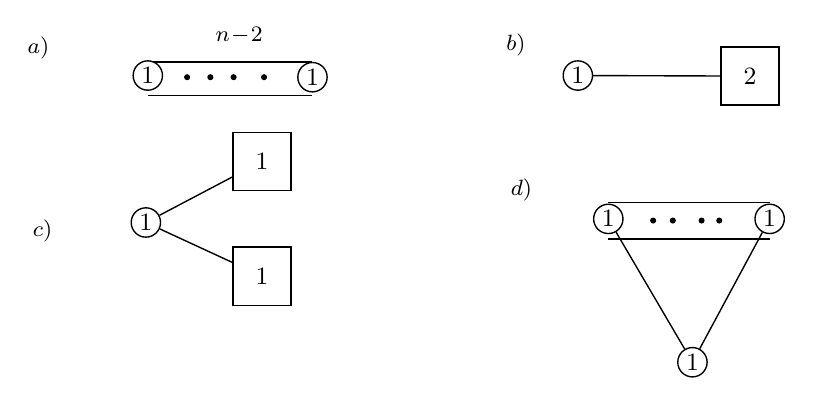
\begin{tikzpicture}[x=1pt,y=1pt,>=stealth,line width=0.5pt,
    nd/.style={circle,draw,fill=white,inner sep=0pt,minimum size=10.6pt,font=\small},
    sq/.style={rectangle,draw,fill=white,inner sep=0pt,minimum size=21pt,font=\small}]
  % ---------------- a) ----------------
  \draw (53,120.4) -- (112.5,120.4);
  \draw (53,108.35) -- (112.5,108.35);
  \node[nd] (a1) at (53,115.5) {1};
  \node[nd] (a2) at (112.5,114.9) {1};
  \foreach \x in {67.2,75.6,84.0,95.0} {\fill (\x,114.9) circle[radius=1.1pt];}
  \node[inner sep=0pt,font=\footnotesize] at (86,129.8) {$n\!-\!2$};
  \node[inner sep=0pt,font=\footnotesize] at (13.5,125.3) {$a)$};
  % ---------------- b) ----------------
  \node[nd] (b1) at (208.4,115.5) {1};
  \node[sq] (b2) at (270.6,115.3) {2};
  \draw (b1) -- (b2);
  \node[inner sep=0pt,font=\footnotesize] at (186,126.6) {$b)$};
  % ---------------- c) ----------------
  \node[nd] (c1) at (52.3,62.4) {1};
  \node[sq] (c2) at (94.3,43.0) {1};
  \node[sq] (c3) at (94.3,84.5) {1};
  \draw (c1) -- (c2);
  \draw (c1) -- (c3);
  \node[inner sep=0pt,font=\footnotesize] at (15,59.2) {$c)$};
  % ---------------- d) ----------------
  \draw (219.4,69.6) -- (277.7,69.6);
  \draw (219.4,56.5) -- (277.7,56.5);
  \node[nd] (d1) at (219.4,63.7) {1};
  \node[nd] (d2) at (277.7,63.7) {1};
  \node[nd] (d3) at (249.8,11.9) {1};
  \draw (d1) -- (d3);
  \draw (d2) -- (d3);
  \foreach \x in {235.6,242.7,253.1,259.5} {\fill (\x,63.1) circle[radius=1.1pt];}
  \node[inner sep=0pt,font=\footnotesize] at (188,74.1) {$d)$};
\end{tikzpicture}

\caption{(a)：极点阶为 $n$ 的 type I 非正则奇点对应的箭图，两个 $U(1)$ 群之间有 $n-2$ 个双基本表示，这就是 $(A_1,A_{N-1})$ 理论的三维镜像，其中 $N=2n-4$；(b)：正则奇点对应的箭图支链；(c)：把 (b) 的 $U(2)$ 味对称性喷开成两个 $U(1)$，以便把这条尾粘到 (a) 的箭图上；(d)：把 c 中的箭图尾与 a 中的箭图粘合，即 $(A_1,D_{N+2})$ 理论的三维镜像。}
\label{fig:4}
\end{figure}

\subsection{由线性箭图得到的 AD 点}
\label{sec:4.3}

在原始文献 \cite{6,11} 中，AD 点是通过调节 $\sN{=}2$ $\SU(2)$ SQCD 库仑分支上的参数找到的。人们自然希望为上一节找到的所有 AD 理论都配上类似的 UV 理论。我们没有去对原理论取各种标度极限，而是借助 Hitchin 系统来看工程化这些理论所需的奇点结构。SQCD 的非正则奇点极点阶较低，而对应的 AD 理论极点阶较高，因此 AD 理论的非正则奇点可以由对应 SQCD 的低阶奇点相撞得到。不过，还是有必要为奇点的碰撞找一条规则。

各种 $\SU(2)$ SQCD 的六维构造已在 \cite{3,41} 中给出。把这些 SQCD 的非正则奇点与相应的 AD 理论作比较，很容易猜出普遍规则，见图 \ref{fig:5}。例如，带一个味的 $\SU(2)$ 有一个 $n=2$ 的 type I 奇点，还有一个同样是 $n=2$ 的 type II 奇点；而对应的 AD 理论只有一个 $n=4$ 的 type II 非正则奇点，它可以看作两个阶为 $2$ 的非正则奇点相撞的结果。关键在于：新非正则奇点所编码的参数个数，应当等于原来两个奇点参数个数之和。这里我们假定原来那些参数（质量、库仑分支参数）全都成为 AD 理论的参数（质量、耦合常数、库仑分支参数）。

分析图 \ref{fig:5} 中其他情形之后，我们得到如下规则。

若至少有三个奇点，只能做下面这种碰撞：
\begin{enumerate}[label=\textup{\alph*.}]
  \item 把一个非正则奇点与一个正则奇点相撞，非正则奇点的极点阶加一，类型不变。
\end{enumerate}
若只剩下两个非正则奇点，则可以：
\begin{enumerate}[label=\textup{\alph*.},start=2]
  \item 把两个极点阶分别为 $n$ 与 $m$ 的非正则奇点相撞，新的非正则奇点极点阶为 $n+m$。
\end{enumerate}

\begin{figure}[tbp]
\centering
% Figure 5 -- A) Hitchin system for SU(2) QCDs (filled dot: type II irregular,
%             circle: type I irregular, cross: regular; number = integer part of pole order)
%             B) singularity structure of the corresponding AD theory
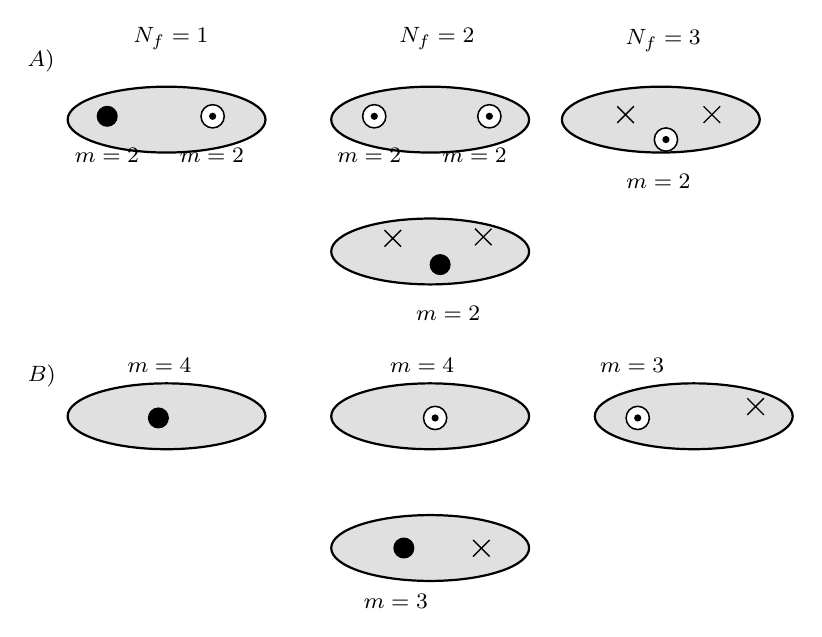
\begin{tikzpicture}[x=1pt,y=1pt,>=stealth,line width=0.5pt,
    ell/.style={draw,fill=black!12,line width=0.8pt}]
  % ================= A) =================
  \node[inner sep=0pt,font=\footnotesize] at (6.9,200.6) {$A)$};
  % N_f = 1
  \draw[ell] (52.25,179.4) ellipse[x radius=35.75pt,y radius=11.9pt];
  \fill (30.8,180.6) circle[radius=3.8pt];
  \draw[line width=0.55pt,fill=white] (68.9,180.6) circle[radius=4.2pt];
  \fill (68.9,180.6) circle[radius=1.3pt];
  \node[inner sep=0pt,font=\footnotesize] at (53.8,208.6) {$N_f=1$};
  \node[inner sep=0pt,font=\footnotesize] at (30.7,166.4) {$m=2$};
  \node[inner sep=0pt,font=\footnotesize] at (68.6,166.4) {$m=2$};
  % N_f = 2
  \draw[ell] (147.5,179.4) ellipse[x radius=35.75pt,y radius=11.9pt];
  \draw[line width=0.55pt,fill=white] (127.3,180.6) circle[radius=4.2pt];
  \fill (127.3,180.6) circle[radius=1.3pt];
  \draw[line width=0.55pt,fill=white] (168.9,180.6) circle[radius=4.2pt];
  \fill (168.9,180.6) circle[radius=1.3pt];
  \node[inner sep=0pt,font=\footnotesize] at (149.9,208.6) {$N_f=2$};
  \node[inner sep=0pt,font=\footnotesize] at (125.5,166.4) {$m=2$};
  \node[inner sep=0pt,font=\footnotesize] at (163.6,166.4) {$m=2$};
  % N_f = 3
  \draw[ell] (230.85,179.4) ellipse[x radius=35.75pt,y radius=11.9pt];
  \draw (215.1,178.2) -- (221.1,184.2);
  \draw (215.1,184.2) -- (221.1,178.2);
  \draw (246.3,178.2) -- (252.3,184.2);
  \draw (246.3,184.2) -- (252.3,178.2);
  \draw[line width=0.55pt,fill=white] (232.7,172.2) circle[radius=4.2pt];
  \fill (232.7,172.2) circle[radius=1.3pt];
  \node[inner sep=0pt,font=\footnotesize] at (231.7,208.0) {$N_f=3$};
  \node[inner sep=0pt,font=\footnotesize] at (230.0,157.0) {$m=2$};
  % second row of A)
  \draw[ell] (147.5,131.75) ellipse[x radius=35.75pt,y radius=11.9pt];
  \draw (131.0,133.5) -- (137.0,139.5);
  \draw (131.0,139.5) -- (137.0,133.5);
  \draw (163.7,134.0) -- (169.7,140.0);
  \draw (163.7,140.0) -- (169.7,134.0);
  \fill (151.1,127.0) circle[radius=3.8pt];
  \node[inner sep=0pt,font=\footnotesize] at (154.0,109.5) {$m=2$};
  % ================= B) =================
  \node[inner sep=0pt,font=\footnotesize] at (7.2,86.7) {$B)$};
  % m = 4 (type II)
  \draw[ell] (52.25,72.2) ellipse[x radius=35.75pt,y radius=11.9pt];
  \fill (49.3,71.6) circle[radius=3.8pt];
  \node[inner sep=0pt,font=\footnotesize] at (49.7,90.5) {$m=4$};
  % m = 4 (type I)
  \draw[ell] (147.5,72.2) ellipse[x radius=35.75pt,y radius=11.9pt];
  \draw[line width=0.55pt,fill=white] (149.3,71.6) circle[radius=4.2pt];
  \fill (149.3,71.6) circle[radius=1.3pt];
  \node[inner sep=0pt,font=\footnotesize] at (144.6,90.5) {$m=4$};
  % m = 3 (type I + regular)
  \draw[ell] (242.75,72.2) ellipse[x radius=35.75pt,y radius=11.9pt];
  \draw[line width=0.55pt,fill=white] (222.5,71.6) circle[radius=4.2pt];
  \fill (222.5,71.6) circle[radius=1.3pt];
  \draw (262.1,72.7) -- (268.1,78.7);
  \draw (262.1,78.7) -- (268.1,72.7);
  \node[inner sep=0pt,font=\footnotesize] at (220.5,90.5) {$m=3$};
  % second row of B)
  \draw[ell] (147.5,24.6) ellipse[x radius=35.75pt,y radius=11.9pt];
  \fill (138,24.6) circle[radius=3.8pt];
  \draw (163.0,21.5) -- (169.0,27.5);
  \draw (163.0,27.5) -- (169.0,21.5);
  \node[inner sep=0pt,font=\footnotesize] at (135.1,5.2) {$m=3$};
\end{tikzpicture}

\caption{A)：各种 $\SU(2)$ QCD 的 Hitchin 系统，黑点代表 type II 非正则奇点，圆圈代表 type I 非正则奇点，叉号代表正则奇点，数字是极点阶的整数部分。B)：由上述 QCD 找到的相应 AD 理论的奇点结构。}
\label{fig:5}
\end{figure}

利用上面的规则，不难为前面构造的 AD 理论找出 UV 理论。库仑分支为 $(n-1)$ 维的 AD 理论共有四个：$(A_1,A_{2n-1})$、$(A_1,A_{2n-2})$、$(A_1,D_{2n})$、$(A_1,D_{2n-1})$。按上述规则，可以定出其中一类理论的 UV 理论。其 UV 理论是 $\SU(2)-\SU(2)$ 线性箭图，两端挂不同数目的基本表示：
\begin{align}
\text{1. } &(A_1,A_{2n-2}) \to 0 - \underbrace{\SU(2)-\cdots-\SU(2)}_{n-1} - 1 ,\notag\\
\text{2. } &(A_1,A_{2n-1}) \to 1 - \underbrace{\SU(2)-\cdots-\SU(2)}_{n-1} - 1 ,\notag\\
\text{3. } &(A_1,D_{2n-1}) \to 0 - \underbrace{\SU(2)-\cdots-\SU(2)}_{n-1} - 2 ,\notag\\
\text{4. } &(A_1,D_{2n})   \to 1 - \underbrace{\SU(2)-\cdots-\SU(2)}_{n-1} - 2 .
\end{align}

下面解释第 1 种情形的碰撞规则，其他理论可类似理解。该线性箭图理论有一个阶为 $2$ 的 type I 奇点、一个阶为 $2-1/2$ 的 type II 奇点，以及 $n-2$ 个正则奇点。先把 type I 奇点与那些正则奇点相撞，得到一个阶为 $n$ 的 type I 奇点；最后再与 type II 奇点相撞，得到一个更高阶（$n+3/2$）的 type II 奇点，它正是 $(A_1,A_{2n-2})$ 理论所需的那个。UV 理论总共有 $2n-2$ 个参数，红外理论同样有 $2n-2$ 个参数。

\subsection{中心荷 $a$ 与 $c$}
\label{sec:4.4}

计算本节构造的 AD 理论的中心荷 $a$ 与 $c$，有两条路。第一条是使用下面两个公式
\begin{equation}
(2a-c) = \frac{1}{4}\sum_{i=1}^{r}\bigl(2D(u_i)-1\bigr),\qquad
a-c = \frac{1}{24}(n_v - n_h).
\label{eq:4.8}\tag{4.8}
\end{equation}
第二个公式对弱耦合的自由理论成立；我们假定把 $n_v$ 与 $n_h$ 视为矢量多重态与超多重态的有效个数之后，它对强耦合理论同样成立。注意 $n_v-n_h$ 恰好是 SCFT 的「Higgs」分支维数的相反数。这个数等于镜像理论库仑分支的维数，而镜像有拉氏量描述，故容易计算。对 $N=2n$ 的 $(A_1,A_{N-1})$ 理论，三维镜像的库仑分支维数为一。

先把上面两个公式用到 $(A_1,A_{N-1})$ 理论，得到
\begin{equation}
2a-c = \frac{1}{4}\sum_{i=n+2}^{2n}\Bigl(\frac{4i}{2n+2}-1\Bigr)
= \frac{1}{4}\frac{(-1+n)(1+2n)}{(1+n)},\qquad
a-c = -\frac{1}{24}.
\label{eq:4.9}\tag{4.9}
\end{equation}
解上面的方程组，得到
\begin{equation}
a = \frac{-5-5n+12n^2}{24(1+n)},\qquad
c = \frac{3n^2-n-1}{6(n+1)}.
\label{eq:4.10}\tag{4.10}
\end{equation}
对 $N=2n$ 的 $(A_1,D_{N+2})$ 理论，利用「三维镜像的库仑分支维数为二」这一事实，可以做类似的计算：
\begin{equation}
2a-c = \frac{1}{4}\sum_{i=n+2}^{2n+1}\Bigl(\frac{4i}{2n+2}-1\Bigr) = \frac{n}{2},\qquad
a-c = -\frac{1}{12}.
\label{eq:4.11}\tag{4.11}
\end{equation}
解之即得中心荷
\begin{equation}
a = \frac{n}{2} + \frac{1}{12},\qquad c = \frac{n}{2} + \frac{1}{6}.
\label{eq:4.12}\tag{4.12}
\end{equation}

要计算 $N = 2n-1$ 时的中心荷，我们使用下面这个由拓扑场论导出的公式 \cite{20}：
\begin{equation}
a = \frac{1}{4}R(A) + \frac{1}{6}R(B) + \frac{5}{24}r,\qquad
c = \frac{1}{3}R(B) + \frac{1}{6}r,
\label{eq:4.13}\tag{4.13}
\end{equation}
其中 $r$ 是库仑分支的维数，而 AD 理论的 $h$ 为零；又
\begin{equation}
R(A) = \sum_{i}\bigl(D(u_i)-1\bigr),
\label{eq:4.14}\tag{4.14}
\end{equation}
这里的求和跑遍所有库仑分支算子，用显式的 Seiberg--Witten 曲线容易算出。$R(B)$ 与 Seiberg--Witten 曲线的判别式有关，一般极难计算。我们的想法是：假设 $R(B)$ 对每一类理论都是 $N$ 的普适函数，再利用 $N=2n$ 时的上述结果，定出 $R(B)$ 对 $N$ 的函数依赖关系。

\typo{原文 p.19 在式 (4.13) 前写「the following formula derived from topological field theory (3)」，其中引用的「(3)」编号有误；从上下文看，它指的是第 \ref{sec:general} 节的式 (2.8)。译文按 (2.8) 理解，并在此注出。后文 p.22 又两次以「formula (3)」指同一式。}

对 $N=2n$ 的 $(A_1,A_{N-1})$ SCFT，用 Seiberg--Witten 曲线给出的算子标度维数，得到（另见 \cite{42}）
\begin{equation}
N = 2n:\quad R(A) = \frac{n(n-1)}{2(n+1)}.
\label{eq:4.15}\tag{4.15}
\end{equation}
把已知的中心荷 $a$ 与 $c$ 代入上面那个公式，即得 $R(B)$ 的形式
\begin{equation}
(A_1,A_{N-1}):\quad R(B) = \frac{N(N-1)}{2(N+2)}.
\label{eq:4.16}\tag{4.16}
\end{equation}
类似地，对 $(A_1,D_N)$ 理论容易算出
\begin{equation}
N = 2n:\quad R(A) = \frac{n}{2},
\label{eq:4.17}\tag{4.17}
\end{equation}
并得到 $R(B)$ 的如下结果：
\begin{equation}
(A_1,D_{N+2}):\quad R(B) = \frac{N+1}{2}.
\label{eq:4.18}\tag{4.18}
\end{equation}
于是终于可以算出那些我们没有三维镜像构造的理论的中心荷，只需用 $R(B)$ 的显式形式。$N=2n-1$ 时 AD 理论的中心荷为
\begin{equation}
\begin{aligned}
(A_1,A_{N-1}):\quad & a = \frac{(n-1)(24n-5)}{24(2n+1)},\quad c = \frac{(n-1)(6n-1)}{6(2n+1)};\\
(A_1,D_{N+2}):\quad & a = \frac{n(8n+3)}{8(2n+1)},\quad c = \frac{n}{2}.
\end{aligned}
\label{eq:4.19}\tag{4.19}
\end{equation}
上述结果与 \cite{20,42} 完全一致。一个自洽性检验是：$(A_1,D_3)$ 与 $(A_1,A_3)$ 两个理论给出相同的答案，$a=\tfrac{11}{24}$、$c=\tfrac{1}{2}$。中心荷公式汇总在表 \ref{tab:3} 中。

\begin{table}[tbp]
\centering
\caption{由六维 $A_1$ $(2,0)$ 理论得到的 AD 理论的中心荷。}
\label{tab:3}
\begin{tabular}{llcc}
\toprule
 & 约束 & $a$ & $c$\\
\midrule
$(A_1,A_{N-1})$ & $N=2n$   & $\dfrac{-5-5n+12n^2}{24(1+n)}$ & $\dfrac{3n^2-n-1}{6(n+1)}$\\[6pt]
$(A_1,A_{N-1})$ & $N=2n-1$ & $\dfrac{(n-1)(24n-5)}{24(2n+1)}$ & $\dfrac{(n-1)(6n-1)}{6(2n+1)}$\\[6pt]
$(A_1,D_{N+2})$ & $N=2n$   & $\dfrac{n}{2}+\dfrac{1}{12}$ & $\dfrac{n}{2}+\dfrac{1}{6}$\\[6pt]
$(A_1,D_{N+2})$ & $N=2n-1$ & $\dfrac{n(8n+3)}{8(2n+1)}$ & $\dfrac{n}{2}$\\
\bottomrule
\end{tabular}
\end{table}

\subsection{更多奇点：与 $(A_1,D_{N+2})$ 理论耦合的规范理论}
\label{sec:4.5}

我们可以在任意黎曼面上放任意多个非正则奇点与正则奇点。这些理论是渐近自由理论；若把非阿贝尔味对称性规范化，这一点可以用 AD 理论对 $\beta$ 函数的贡献来确认 \cite{22}。物理上，物质部分是带正则穿刺点的三孔球（代表三基本表示），以及带一个非正则奇点与一个正则奇点的球（代表 AD 理论）。整个理论由把正则奇点的对角 $\SU(2)$ 味对称性规范化得到，例子见图 \ref{fig:6}。

在球上只有一个 type I 非正则奇点、外加若干正则奇点的情形，可以用前面讲的那套处方求出它的三维镜像，一个例子见图 \ref{fig:7}。这些理论被称为完备理论，其 BPS 谱已在 \cite{31} 中研究过；特别是，这些理论的 BPS 箭图属于有限变异型 \cite{43}。

\begin{figure}[tbp]
\centering
% Figure 6 -- (a) Riemann sphere with one irregular and two regular punctures,
%             (b) its degeneration limit: two fundamentals and an AD point
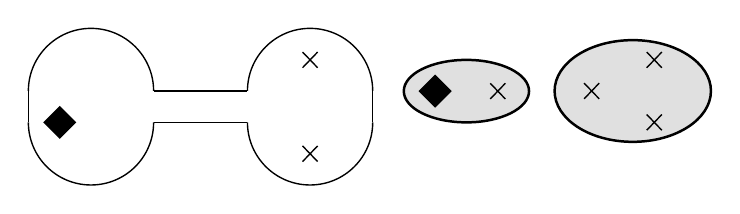
\begin{tikzpicture}[x=1pt,y=1pt,scale=1.05,transform shape,>=stealth,line width=0.5pt,
    bulb/.style={line width=0.5pt}, grey/.style={draw,fill=black!12,line width=0.9pt}]
  \def\cross#1#2{\draw (#1-2.6,#2-2.7) -- (#1+2.6,#2+2.7);\draw (#1-2.6,#2+2.7) -- (#1+2.6,#2-2.7);}
  % ---------- (a) dumbbell ----------
  \draw (51.6,35.0) arc[start angle=180,end angle=0,radius=21.55];
  \draw (51.6,24.2) arc[start angle=180,end angle=360,radius=21.55];
  \draw (51.6,24.2) -- (51.6,35.0);
  \draw (94.7,24.2) -- (127.0,24.2);
  \draw (94.7,35.0) -- (127.0,35.0);
  \draw (127.0,35.0) arc[start angle=180,end angle=0,radius=21.55];
  \draw (127.0,24.2) arc[start angle=180,end angle=360,radius=21.55];
  \draw (170.1,24.2) -- (170.1,35.0);
  % irregular puncture (filled diamond)
  \fill (56.7,24.2) -- (62.4,29.9) -- (68.1,24.2) -- (62.4,18.5) -- cycle;
  % two regular punctures
  \cross{148.55}{13.4}
  \cross{148.55}{45.7}
  % ---------- (b) the two pieces ----------
  \draw[grey] (202.35,34.95) ellipse[x radius=21.55pt,y radius=10.75pt];
  \fill (185.9,34.95) -- (191.6,40.65) -- (197.3,34.95) -- (191.6,29.25) -- cycle;
  \cross{213.15}{34.95}
  \draw[grey] (259.6,35.0) ellipse[x radius=26.9pt,y radius=17.5pt];
  \cross{245.45}{35.0}
  \cross{267}{24.2}
  \cross{267}{45.7}
\end{tikzpicture}

\caption{(a) 带一个非正则穿刺点与两个正则穿刺点的黎曼球。(b) 在它的「退化极限」下，物质是两个基本表示加上我们前面定义的一个 AD 点。}
\label{fig:6}
\end{figure}

\begin{figure}[tbp]
\centering
% Figure 7 -- the three dimensional mirror of the gauge theory of figure 6
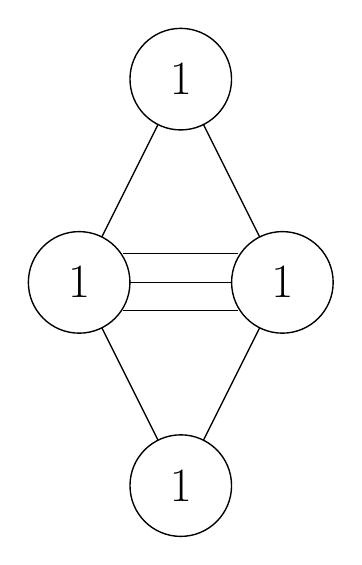
\begin{tikzpicture}[x=1.8pt,y=1.8pt,>=stealth,line width=0.5pt,
    nd/.style={circle,draw,fill=white,inner sep=0pt,minimum size=36.7pt,
               font=\fontsize{16.4}{19}\selectfont}]
  % the two horizontal links between the left and the right node
  \draw (24.4,47.7) -- (47.4,47.7);
  \draw (24.4,59.2) -- (47.4,59.2);
  % the four legs
  \draw (15.5,53.4) -- (35.9,94.2);
  \draw (35.9,94.2) -- (56.3,53.4);
  \draw (15.5,53.4) -- (35.9,12.6);
  \draw (35.9,12.6) -- (56.3,53.4);
  \draw (25.7,53.4) -- (46.1,53.4);
  % nodes
  \node[nd] at (15.5,53.4) {1};
  \node[nd] at (56.3,53.4) {1};
  \node[nd] at (35.9,94.2) {1};
  \node[nd] at (35.9,12.6) {1};
\end{tikzpicture}

\caption{上一图所述规范理论的三维镜像。}
\label{fig:7}
\end{figure}


% =====================================================================
%  sections/sec5.tex —— 5 由六维 A_2 理论得到的 AD 点（原文 pp.22–31）
% =====================================================================
\section{由六维 $A_2$ 理论得到的 AD 点}
\label{sec:a2}

现在我们从六维 $A_2$ 理论出发，把它紧致化在带非正则奇点的黎曼面上，希望在红外得到一个四维 AD 理论。关于黎曼面的类型与非正则奇点数目的分析，与 $\SU(2)$ 情形完全相同，只要盯住 Seiberg--Witten 曲线中的二次微分即可。我们同样只能用黎曼球，并且只能有一个非正则奇点，或一个非正则奇点加一个正则奇点。$A_2$ 理论中非正则奇点的可选类型比 $A_1$ 理论里仅有的两种要多，因此我们立刻得到许多新的 AD 型理论。

\subsection{AD 理论的非正则奇点分类}
\label{sec:5.1}

按照我们对非正则奇点的分类，$\SU(3)$ 群的非正则奇点有如下几种：

\textbf{Type I：}非正则奇点的极点阶与领头阶矩阵为
\begin{equation}
\Phi = z^{r-2}\diag(1,\ \omega,\ \omega^2),\qquad r = n + j/3,\quad 0<j\le 3 .
\label{eq:5.1}\tag{5.1}
\end{equation}
当极点阶为整数时，领头阶矩阵不必具有上述特定形式，其对角元可以取任意三个数；此时还有两个质量参数编码在一阶极点的系数里。若极点阶为分数，则没有质量参数。耦合常数的个数（不含领头阶与一阶极点的系数）由「数出所有与领头阶矩阵相容的形变」得到：
\begin{equation}
\Ncoupling = 2n+j-3\ \ (j\ne 3),\qquad
\Ncoupling = 2(n-1)\ \ (j = 3).
\label{eq:5.2}\tag{5.2}
\end{equation}
这类非正则奇点的牛顿多边形见图 \ref{fig:8}a。

\textbf{Type II：}非正则奇点的极点阶与领头阶矩阵为
\begin{equation}
\Phi = z^{r-2}\diag(0,\ 1,\ \omega),\qquad r = n + 1/2 .
\label{eq:5.3}\tag{5.3}
\end{equation}
一阶极点的系数给出一个质量参数，而耦合常数的个数为
\begin{equation}
\Ncoupling = 2(n-1).
\label{eq:5.4}\tag{5.4}
\end{equation}
这类非正则奇点的牛顿多边形见图 \ref{fig:8}b。

\textbf{Type III：}可以考虑极点阶为整数 $n$ 的非正则奇点的退化。此时非正则奇点由两个整数 $(n_1,n_2)$ 标记，且 $n_1+n_2 = n$，即它含有 $n_1$ 个单杨图与 $n_2$ 个满杨图。质量参数的个数由杨图 $Y_1$ 定：$Y_1$ 是单杨图时有一个，是满杨图时有两个。耦合常数的个数为
\begin{equation}
\Ncoupling = n_1 + 2n_2 - 3 .
\label{eq:5.5}\tag{5.5}
\end{equation}
以上信息汇总在表 \ref{tab:4} 中。

\begin{table}[tbp]
\centering
\caption{由几何数据数参数。这里数的是非正则奇点高阶系数中可能的最大参数个数。}
\label{tab:4}
\begin{tabular}{lcccc}
\toprule
 & 极点阶 & 底空间维数 & 一阶极点 & 高阶极点\\
\midrule
Type I   & $n+j/3$        & $3n+j-7$        & 0 & $2n-3+j$\\
Type I   & $n+1$          & $3n-5$          & 2 & $2(n-1)$＋一个边缘项\\
Type II  & $n+1/2$        & $\frac{3}{2}(n-1)$ & 1 & $2(n-1)$\\
Type III & $n = n_1+n_2$  & $2n_1+n_2-8$    & 2 或 1 & $n_1+2n_2-3$\\
\bottomrule
\end{tabular}
\end{table}

\typo{表 4 的「底空间维数」一栏与正文对不上。按第 \ref{sec:5.1.3} 小节的式 (5.19)，库仑分支维数为 $d = 2n_1+3n_2-8 = 2n+n_2-8$，而表中 Type III 行给的是 $2n_1+n_2-8$；Type II 行给的是 $\frac{3}{2}(n-1)$，对整数 $n$ 并不是整数，按 $\SU(2)$ 情形的同类记账应为 $3n-3$。此处照录原文，未作改动。}

\subsubsection{Type I SCFT：$(A_2,A_{N-1})$ 理论}
\label{sec:5.1.1}

把六维 $A_2$ 理论紧致化在带第一类非正则奇点的黎曼球上，红外就得到一个四维 AD 理论。Seiberg--Witten 曲线可以很容易地用穿刺点上 Higgs 场的形式，从谱曲线求出。实际上，直接从相应非正则奇点的牛顿多边形读出它更方便。牛顿多边形所界定的格点，代表 Seiberg--Witten 曲线中允许出现的单项式。我们用标度不变性把 $z^N$ 项的系数取为一，用平移不变性消去 $z^{N-1}$ 项。$x=2$ 这条线上的点不用，因为 Higgs 场的迹为零。

$(A_2,A_{N-1})$ 理论由 Seiberg--Witten 曲线 $x^3+z^N=0$ 描述，而坐标的标度维数由「要求 Seiberg--Witten 微分 $\lambda = x\,\dd z$ 的维数为一」定出：
\begin{equation}
[x] = \frac{N}{N+3},\qquad [z] = \frac{3}{N+3}.
\label{eq:5.6}\tag{5.6}
\end{equation}
Seiberg--Witten 曲线可以由图 \ref{fig:9} 中牛顿多边形所界定的整数点读出：每个含于其内的点，坐标为 $(m,n)$，对应 Seiberg--Witten 曲线中的一个单项式 $x^mz^n$。

\begin{figure}[tbp]
\centering
% Figure 8 -- a: Newton polygon of the type I irregular singularity
%             b: Newton polygon of the type II irregular singularity
\begin{tikzpicture}[x=1pt,y=1pt,>=stealth,line width=0.5pt]
  \def\u{18.7}
  % ---------------- a) ----------------
  \begin{scope}[shift={(26.2,3.8)}]
    \draw (0,0) -- (0,{6.03*\u});
    \draw (0,0) -- ({4.03*\u},0);
    \foreach \j in {0,...,5} {\fill (0,{\j*\u}) circle[radius=1.9pt];}
    \foreach \i in {1,2,3} {\fill ({\i*\u},0) circle[radius=1.9pt];}
    \draw (0,{5*\u}) -- ({3*\u},0);
  \end{scope}
  \node[inner sep=0pt,font=\fontsize{10.5}{13}\selectfont] at (10.5,110.8) {$a$};
  % ---------------- b) ----------------
  \begin{scope}[shift={(175.7,3.8)}]
    \draw (0,0) -- (0,{6.03*\u});
    \draw (0,0) -- ({6.03*\u},0);
    \foreach \j in {0,...,4} {\fill (0,{\j*\u}) circle[radius=1.9pt];}
    \foreach \i in {1,2,3} {\fill ({\i*\u},0) circle[radius=1.9pt];}
    \fill ({\u},{3*\u}) circle[radius=1.9pt];
    \draw (0,{4*\u}) -- ({\u},{3*\u}) -- ({3*\u},0);
  \end{scope}
  \node[inner sep=0pt,font=\fontsize{10.5}{13}\selectfont] at (150.6,110.8) {$b$};
\end{tikzpicture}

\caption{a：type I 非正则奇点的牛顿多边形。b：type II 非正则奇点的牛顿多边形。}
\label{fig:8}
\end{figure}

一般形变下的 Seiberg--Witten 曲线，用牛顿多边形所界定的格点求出。我们取 $N = 3n-1$ 作详细例子，其他情形类似。Seiberg--Witten 曲线为
\begin{equation}
x^3 + \bigl(v_1z^{2n-1} + \cdots + v_iz^{2n-i} + \cdots + v_{2n}\bigr)x
+ \bigl(z^{3n-1} + u_1z^{3n-3} + \cdots + u_{3n-2}\bigr) = 0 .
\label{eq:5.7}\tag{5.7}
\end{equation}
利用坐标的标度维数，可以求出 Seiberg--Witten 曲线中出现的各种算子的标度维数：
\begin{equation}
[v_i] = \frac{3i-2}{3n+2},\qquad [u_i] = \frac{3+3i}{3n+2}.
\label{eq:5.8}\tag{5.8}
\end{equation}
容易看出：对谱中每一个相关算子 $\sO_i$，都存在另一个耦合常数 $m_i$，使 $D(\sO_i)+D(m_i)=2$。谱中没有质量参数，库仑分支的维数为 $3n-2$；此外还有 $2n$ 个维数小于一的算子，它们是相关形变的耦合常数。

下面把上述数字与非正则奇点定义中的参数作比较。该非正则奇点的极点阶为
\begin{equation}
r = (3n-1)/3 + 2 = (n+1) + 2/3 .
\label{eq:5.9}\tag{5.9}
\end{equation}
由于极点阶是分数，这里没有质量参数，与从 Seiberg--Witten 曲线得到的结果吻合得很好。

来自非正则奇点的耦合常数总数是 $2n+1$ 个。用平移不变性减去一个耦合常数，最终的数字与从 Seiberg--Witten 曲线得到的结果一致。也可以检验：库仑分支的维数与 Hitchin 纤维化底空间的维数相同。

\begin{figure}[tbp]
\centering
% Figure 9 -- lattice points bounded by the Newton polygon, for the three cases a, b, c
\begin{tikzpicture}[x=1pt,y=1pt,>=stealth,line width=0.4pt]
  % ================= a =================
  \begin{scope}[shift={(43.2,152.7)}]
    \def\u{12.75}\def\dd{1.2}\def\oo{2.0}
    \foreach \j in {0,...,6} {\draw (0,{\j*\u}) -- ({7.04*\u},{\j*\u});}
    \foreach \i in {0,...,3} {\draw ({\i*\u},0) -- ({\i*\u},{8.02*\u});}
    \foreach \i/\j in {0/0,1/0,3/0,0/1,1/1,0/2,1/2,0/3,1/3,0/4,0/6}
      {\fill ({\i*\u},{\j*\u}) circle[radius=\dd pt];}
    \foreach \i/\j in {2/0,2/1,0/5} {\draw[fill=white] ({\i*\u},{\j*\u}) circle[radius=\oo pt];}
    \draw[line width=0.8pt] (0,{6*\u}) -- ({3*\u},0);
  \end{scope}
  \node[inner sep=0pt,font=\fontsize{9.6}{12}\selectfont] at (20.4,245.8) {$a$};
  % ================= b =================
  \begin{scope}[shift={(209.0,152.7)}]
    \def\u{12.75}\def\dd{1.2}\def\oo{2.0}
    \foreach \j in {0,...,6} {\draw (0,{\j*\u}) -- ({7.04*\u},{\j*\u});}
    \foreach \i in {0,...,2} {\draw ({\i*\u},0) -- ({\i*\u},{8.02*\u});}
    \foreach \i/\j in {0/0,1/0,3/0,0/1,1/1,0/2,0/3,1/3,0/4,0/5,0/6}
      {\fill ({\i*\u},{\j*\u}) circle[radius=\dd pt];}
    \foreach \i/\j in {2/0,2/1,1/2} {\draw[fill=white] ({\i*\u},{\j*\u}) circle[radius=\oo pt];}
    \draw[line width=0.8pt] (0,{4*\u}) -- ({\u},{3*\u}) -- ({3*\u},0);
  \end{scope}
  \node[inner sep=0pt,font=\fontsize{9.6}{12}\selectfont] at (173.4,245.8) {$b$};
  % ================= c =================
  \begin{scope}[shift={(119.8,50.7)}]
    \def\u{12.7}\def\dd{1.2}\def\oo{2.0}
    \draw (0,0) -- ({6.04*\u},0);
    \foreach \j in {1,2,3,4} {\draw (0,{\j*\u}) -- ({4.04*\u},{\j*\u});}
    \draw (0,0) -- (0,{6.05*\u});
    \draw ({\u},{-3.03*\u}) -- ({\u},{6.05*\u});
    \foreach \i in {2,3} {\draw ({\i*\u},0) -- ({\i*\u},{6.05*\u});}
    \foreach \i/\j in {0/-3,0/-2,1/-2,0/-1,1/-1,0/0,1/0,3/0,0/1,1/1,0/2,1/2,0/3,1/3,0/4}
      {\fill ({\i*\u},{\j*\u}) circle[radius=\dd pt];}
    \foreach \i/\j in {2/-1,2/0,2/1} {\draw[fill=white] ({\i*\u},{\j*\u}) circle[radius=\oo pt];}
    \draw[line width=0.8pt] (0,{-3*\u}) -- ({3*\u},0) -- (0,{4*\u});
  \end{scope}
  \node[inner sep=0pt,font=\fontsize{9.6}{12}\selectfont] at (58.4,105.5) {$c$};
  % the label of the lattice
  \node[inner sep=0pt,font=\fontsize{9.6}{12}\selectfont] at (33.9,194.7) {$N$};
\end{tikzpicture}

\caption{Seiberg--Witten 曲线可以从牛顿多边形所界定的整数点读出。每个含于其内的点，坐标为 $(m,n)$，都对应 Seiberg--Witten 曲线中的一个单项式 $x^mz^n$。}
\label{fig:9}
\end{figure}

应当指出，$(A_2,A_3)$ 理论与 $(A_1,E_6)$ 理论等价，这一点文献 \cite{17} 也讨论过。在 AD 点处，Seiberg--Witten 曲线为
\begin{equation}
x^3 + z^4 = 0 .
\label{eq:5.10}\tag{5.10}
\end{equation}
该理论所有算子的标度维数有公分母 $7$。$(A_2,A_4)$ 理论与 $(A_1,E_8)$ 理论同构，因为不动点处的 Seiberg--Witten 曲线为
\begin{equation}
x^3 + z^5 = 0 ,
\label{eq:5.11}\tag{5.11}
\end{equation}
而标度维数的公分母为 $8$，与文献 \cite{17} 的结论一致。用我们的方法可以构造这两个理论的全部形变；此外，利用非正则奇点中的信息可以直接构造 BPS 箭图，而它们确实具有相应 Dynkin 图的形状 \cite{30}。

\subsubsection{Type II SCFT}
\label{sec:5.1.2}

这一类理论用第二类非正则奇点构造。Seiberg--Witten 曲线同样容易由图 \ref{fig:8}b 的牛顿多边形求出，此时 $N = 2n-1$：
\begin{equation}
x^3 + \bigl(z^{2n-1} + v_1z^{2n-3} + \cdots + v_iz^{2n-2-i} + \cdots + v_{2n-2}\bigr)x
+ \bigl(u_1z^{3n-2} + \cdots + u_iz^{3n-1-i} + \cdots + u_{3n-1}\bigr) = 0 .
\label{eq:5.12}\tag{5.12}
\end{equation}
现在标度维数由奇点 $x^3+z^{2n-1}x=0$ 定出，并要求 Seiberg--Witten 微分 $\lambda = x\,\dd z$ 的维数为一，于是
\begin{equation}
[x] = \frac{2n-1}{2n+1},\qquad [z] = \frac{2}{2n+1}.
\label{eq:5.13}\tag{5.13}
\end{equation}
Seiberg--Witten 曲线中各参数的标度维数也容易求出：
\begin{equation}
[v_i] = \frac{2i+2}{2n+1},\qquad [u_i] = \frac{2i-1}{2n+1}.
\label{eq:5.14}\tag{5.14}
\end{equation}
可以验证：对每个相关算子 $u_i$，都存在一个耦合常数 $m_i$，使 $D(m_i)+D(u_i)=2$。谱中有一个质量参数，与表 \ref{tab:4} 的结论一致。该非正则奇点的极点阶为
\begin{equation}
r = \frac{2n-1}{2} + 2 = (n+1) + \frac{1}{2},
\label{eq:5.15}\tag{5.15}
\end{equation}
因此由表 \ref{tab:4}，非正则奇点中共有 $2n$ 个耦合常数；其中一个可以用平移不变性消去，于是几何给出 $2n-1$ 个参数，与从 Seiberg--Witten 曲线读出的耦合常数个数完全吻合。

\subsubsection{Type III SCFT}
\label{sec:5.1.3}

这一类理论用极点阶为整数 $n$ 的第三类奇点来定义：非正则奇点的前 $n_1$ 个矩阵具有分割 $[2,1]$，后 $n_2$ 个系数具有分割 $[1,1,1]$。Seiberg--Witten 曲线与「领头阶奇点为正则半单」的情形相同，但并非曲线中所有算子都是独立的。

Seiberg--Witten 曲线具有如下形式
\begin{equation}
x^3 + \phi_2(z)x + \phi_3(z) = 0 .
\label{eq:5.16}\tag{5.16}
\end{equation}
我们想算出 $\phi_i(z)$ 中 $z$ 的最高幂次 $d_i$，其系数给出独立的库仑分支算子；这个幂次可以从杨图读出。对单个杨图，它对 $\phi_i(z)$ 的贡献是
\begin{equation}
p_i = i - s_i,
\label{eq:5.17}\tag{5.17}
\end{equation}
其中 $s_i$ 是第 $i$ 个格子的高度。对分割 $[2,1]$，有 $p_2=1$、$p_3=1$；对分割 $[1,1,1]$，极点阶为 $p_2=1$、$p_3=2$。代表独立库仑分支参数的领头项，由下式定出
\begin{equation}
d_i = \sum_j p_i^{(j)} - 2i,
\label{eq:5.18}\tag{5.18}
\end{equation}
求和跑遍非正则奇点定义中出现的所有杨图。于是 $d_2 = n-4$、$d_3 = n_1+2n_2-6$，库仑分支的维数为
\begin{equation}
d = d_2 + d_3 + 2 = 2n_1 + 3n_2 - 8 = 2n + n_2 - 8 .
\label{eq:5.19}\tag{5.19}
\end{equation}

\zhnote{[译者按（无外部依据）：按 (5.17) 的字面读法，$[1,1,1]$（高为三的单列）给出 $s_1=1,s_2=2,s_3=3$，从而 $p_2=p_3=0$，与正文所给 $p_2=1$、$p_3=2$ 不合。正文那组数字恰好是「把 $[1,1,1]$ 当作一行三格」读出的结果（此时三个格子的高度都是 $1$，故 $p_i=i-1$），而也只有这组数字代入 (5.18) 才能得到下文所印的 $d_2=n-4$、$d_3=n_1+2n_2-6$。]}%

AD 点处的 Seiberg--Witten 曲线为 $x^3+z^{3n-6}=0$，$[x]$ 与 $[z]$ 的标度维数为
\begin{equation}
[x] = \frac{n-2}{n-1},\qquad [z] = \frac{1}{n-1},
\label{eq:5.20}\tag{5.20}
\end{equation}
而出现在 $\phi_2$ 与 $\phi_3$ 中的库仑分支算子的最小标度维数为
\begin{equation}
[u_1] = 2[x] - d_2[z] = \frac{n}{n-1},\qquad
[v_1] = 3[x] - d_3[z] = \frac{2n-n_2}{n-1}.
\label{eq:5.21}\tag{5.21}
\end{equation}
于是来自 $\phi_2$ 的相关算子有 $(n-3)$ 个，来自 $\phi_3$ 的相关算子有 $n_2-2$ 个。相关算子的总数为
\begin{equation}
N_{\text{relevant}} = n-3+n_2-2 = n_1+2n_2-5 .
\label{eq:5.22}\tag{5.22}
\end{equation}
非正则奇点定义中的参数个数为 $n_1+2n_2-3$，可见来自非正则奇点的耦合常数是够用的，只是其中有两个被冻结了。

然而，这些理论并不全是 SCFT。原因在于：几何数据里没有严格边缘形变，而库仑分支的谱却可能由标度维数为二的算子构成。我们的解释是，这些理论是渐近自由理论。不含维数为二的算子的理论对应于 $n_2=1$ 或 $n_2=0$，它们给出新的 SCFT。

\subsubsection{Type IV：一个正则奇点加一个非正则奇点}
\label{sec:5.1.4}

我们可以在此前那个只有一个非正则奇点的例子上，再在 $0$ 点加一个正则奇点。就以\allowbreak $(A_1,A_{3n-1})$ 为例，其他情形完全类似。加上一个满正则奇点之后，Seiberg--Witten 曲线为
\begin{equation}
\begin{aligned}
& x^3 + \Bigl(v_1z^{2n-1} + \cdots v_iz^{2n-i} + v_{2n} + \frac{v_{2n+1}}{z} + \frac{v_{2n+2}}{z^2}\Bigr)x\\
& + \Bigl(z^{3n} + \omega z^{3n-2} + u_1z^{3n-2} + \cdots + u_{3n-1} + \frac{u_{3n}}{z} + \frac{u_{3n+1}}{z^2} + \frac{u_{3n+2}}{z^3}\Bigr) = 0 .
\end{aligned}
\label{eq:5.23}\tag{5.23}
\end{equation}
注意这里出现了一个在单奇点情形被禁的新项 $\omega$。另外还有三个库仑分支参数 $v_{2n+1}$、$u_{3n}$、$u_{3n+1}$，其标度维数为
\begin{equation}
[v_{2n+1}] = \frac{6n+3}{3n+3},\qquad
[u_{3n}] = \frac{9n+3}{3n+3},\qquad
[u_{3n+1}] = \frac{9n+6}{n-1}.
\label{eq:5.24}\tag{5.24}
\end{equation}
$v$ 始终是相关算子。$\omega$ 是一个耦合常数，其标度维数为
\begin{equation}
[\omega] = \frac{3}{3n+3}.
\label{eq:5.25}\tag{5.25}
\end{equation}
于是 $\omega$ 与 $v_{2n+1}$ 恰好配对；另外两个参数 $v_{2n+2}$ 与 $u_{3n+2}$ 则只是质量参数，维数分别为 $2$ 与 $3$。

\typo{式 (5.23) 中 $\omega$ 与 $u_1$ 同时乘在 $z^{3n-2}$ 上，同一幂次出现两个系数，这不可能。由 (5.25) 的 $[\omega]=\frac{3}{3n+3}$ 反推：若 $\omega$ 乘的是 $z^{3n-1}$，则 $[\omega]+(3n-1)[z]=3[x]$ 恰好成立；而 $z^{3n-1}$ 正是单奇点情形被平移不变性消去、加了一个穿刺点之后重新出现的那一项（与 (4.7) 的 $u_1z^{N-1}$ 完全平行）。故原文 $z^{3n-2}$ 应为 $z^{3n-1}$。又 (5.24) 中 $[u_{3n+1}]$ 的分母印作 $n-1$；由单项式 $u_{3n+1}z^{-2}$ 的维数等于 $3[x]$ 反算，分母应为 $3n+3$。两处均照录原文。}

\typo{第 \ref{sec:5.1.4} 小节开头原文写作「就以 $(A_1,A_{3n-1})$ 为例」。本节处理的是六维 $A_2$ 理论，且式 (5.23) 的曲线与 $(A_2,A_{3n-1})$ 相符，故此处下标 $1$ 应为 $2$。译文照录原文。}

若正则奇点是单的，则只有 $v_{2n+1}$ 与 $u_{3n}$ 是独立的库仑分支算子，且只有一个新质量参数。

\subsection{三维镜像理论}
\label{sec:5.2}

若把四维理论紧致化在一个圆上并流向深红外，红外理论是一个三维 $\sN{=}4$ SCFT $A$。只要极点阶是整数，就可以直接从非正则奇点求出它的镜像理论 $B$ \cite{44}。设前 $n_1$ 个分割的杨图为 $[2,1]$，后 $n_2$ 个分割的杨图为 $[1,1,1]$，则可以按图 \ref{fig:10} 配上一个箭图。若 $n_2=0$，则只有两个节点，其秩分别为 $1$ 与 $2$，两节点之间有 $n-2$ 支箭；此时原理论的质量参数个数为一。

有几个容易做的检验：该箭图的希格斯分支维数为 $2n+n_2-8$，恰好是原理论的库仑分支；FI 参数的个数正好是箭图节点数减一，与原理论的质量参数个数相符。正则奇点的箭图支链已在 \cite{38} 中给出，它完全由杨图确定，见图 \ref{fig:10}。要把正则奇点的箭图支链粘到非正则奇点的箭图上，需要按非正则奇点箭图的模式把正则奇点的 $U(3)$ 味对称性劈开，即：若非正则奇点的箭图有三个 $U(1)$ 节点，就把正则奇点的 $U(3)$ 味对称性劈成三个 $U(1)$。粘合通过把这些 $U(1)$ 味对称性与非正则奇点箭图的 $U(1)$ 规范群认同来实现。

\begin{figure}[tbp]
\centering
% Figure 10 -- a) U(1)xU(1) with n-2 bifundamentals; b) the regular puncture legs;
%              c) U(2) split into two U(1); d) after gluing
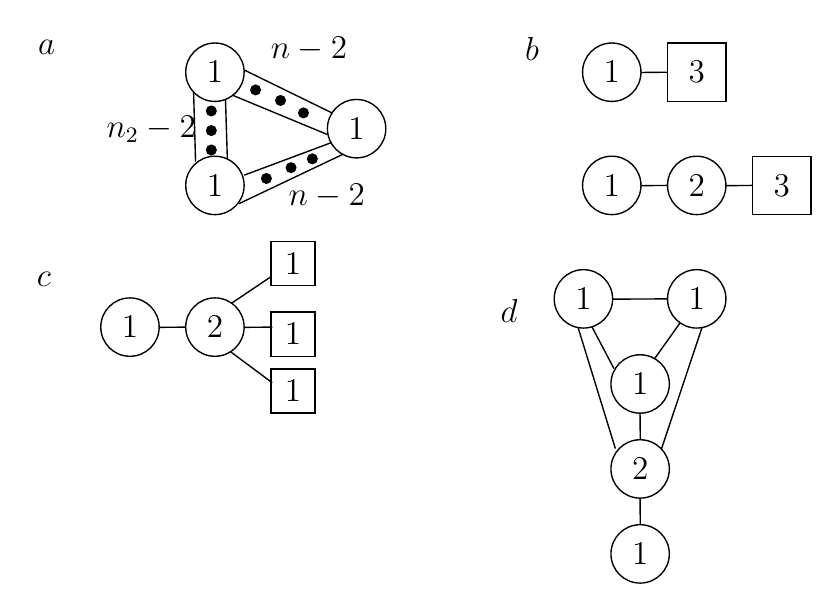
\begin{tikzpicture}[x=1pt,y=1pt,>=stealth,line width=0.5pt,
    nd/.style={circle,draw,fill=white,inner sep=0pt,minimum size=21.1pt,
               font=\fontsize{11.5}{14}\selectfont},
    sq/.style={rectangle,draw,fill=white,inner sep=0pt,minimum width=21.2pt,
               minimum height=21.1pt,font=\fontsize{11.5}{14}\selectfont},
    rr/.style={font=\fontsize{11.5}{14}\selectfont}]
  % =================== a) ===================
  % ribbon between the two left nodes (vertical)
  \draw (65.2,188.5) -- (65.9,163.5);
  \draw (76.7,186.6) -- (77.4,164.1);
  % ribbon to the right node, upper
  \draw (79.0,187.6) -- (113.5,173.3);
  \draw (83.5,196.6) -- (115.4,181.0);
  % ribbon to the right node, lower
  \draw (81.6,148.3) -- (119.9,166.5);
  \draw (83.5,158.6) -- (114.8,170.3);
  \foreach \x/\y in {91.5/157.4, 100.4/161.3, 108.1/164.5,
                     71.6/167.7, 71.6/174.7, 71.6/181.8,
                     104.9/181.1, 96.6/185.6, 87.6/189.4}
    {\fill (\x,\y) circle[radius=2.0pt];}
  \node[nd] at (72.9,195.8) {1};
  \node[nd] at (72.9,154.9) {1};
  \node[nd] at (124.1,175.4) {1};
  \node[rr] at (106.9,204.2) {$n-2$};
  \node[rr] at (113.3,151.1) {$n-2$};
  \node[rr] at (49.9,175.2) {$n_2-2$};
  \node[rr] at (12.1,204.8) {$a$};
  \node[rr] at (187.5,204.2) {$b$};
  % =================== b) ===================
  \draw (226.2,195.7) -- (237.1,195.8);
  \node[nd] at (216.3,195.8) {1};
  \node[sq] at (247.0,195.85) {3};
  \draw (226.2,154.8) -- (237.1,154.9);
  \draw (256.9,154.8) -- (267.8,154.9);
  \node[nd] at (216.3,154.9) {1};
  \node[nd] at (247.0,154.9) {2};
  \node[sq] at (277.75,154.85) {3};
  % =================== c) ===================
  \draw (52.1,103.6) -- (63.0,103.7);
  \draw (82.8,103.6) -- (93.7,103.7);
  \draw (78.4,94.9) -- (93.6,83.6);
  \draw (79.0,112.4) -- (93.0,121.8);
  \draw (93.1,118.7) rectangle (109.1,134.7);
  \draw (93.1,93.1) rectangle (109.1,109.1);
  \draw (93.1,72.6) rectangle (109.1,88.6);
  \node[nd] at (42.2,103.7) {1};
  \node[nd] at (72.9,103.7) {2};
  \node[rr] at (101.1,126.7) {1};
  \node[rr] at (101.1,101.1) {1};
  \node[rr] at (101.1,80.6) {1};
  \node[rr] at (11.1,121.0) {$c$};
  % =================== d) ===================
  \draw (216.0,113.8) -- (237.1,113.9);
  \draw (208.4,105.2) -- (217.1,88.7);
  \draw (231.5,91.9) -- (241.4,105.8);
  \draw (203.4,105.9) -- (217.6,59.8);
  \draw (234.1,59.2) -- (249.7,105.9);
  \draw (226.5,73.9) -- (226.6,63.0);
  \draw (226.5,43.8) -- (226.6,32.3);
  \node[nd] at (206.05,113.9) {1};
  \node[nd] at (247.0,113.9) {1};
  \node[nd] at (226.55,83.15) {1};
  \node[nd] at (226.55,52.45) {2};
  \node[nd] at (226.55,21.75) {1};
  \node[rr] at (179.2,109.5) {$d$};
\end{tikzpicture}

\caption{a：带 $n_1$ 个单杨图与 $n_2$ 个满杨图、极点阶为 $n=n_1+n_2$ 的非正则奇点所对应的箭图。b：单正则穿刺点与满正则穿刺点所对应的箭图支链。c：把正则奇点箭图支链的 $U(3)$ 味对称性劈成三个 $U(1)$ 因子。d：把劈开后的正则奇点箭图支链粘到非正则奇点上，构成三维镜像理论；这里有一个阶为 $3$、领头阶为正则半单的非正则奇点，还有一个满正则奇点。}
\label{fig:10}
\end{figure}

\subsection{中心荷 $a$ 与 $c$}
\label{sec:5.3}

求中心荷 $a$ 与 $c$ 的策略与我们在 $\SU(2)$ 理论中做的完全一样：先用三维镜像对称算出中心荷，再用结果找出这一类理论的普适函数 $R(B)$；最后用 $R(B)$ 算出这一类中其他理论的中心荷。

我们先考虑 $N=3n$ 的 $(A_2,A_{N-1})$ 理论，因为它的三维镜像理论是已知的。用牛顿多边形写出的 Seiberg--Witten 曲线具有如下形式：
\begin{equation}
x^3 + \bigl(v_1z^{2n-1} + \cdots v_iz^{2n-i} + v_{2n}\bigr)x
+ \bigl(z^{3n} + u_1z^{3n-2} + \cdots + u_{3n-1}\bigr) = 0 .
\label{eq:5.26}\tag{5.26}
\end{equation}
$x$ 与 $z$ 的标度维数为
\begin{equation}
[x] = \frac{3n}{3n+3},\qquad [z] = \frac{3}{3n+3}.
\label{eq:5.27}\tag{5.27}
\end{equation}
用这些信息可以求出各算子的标度维数：
\begin{equation}
[v_i] = \frac{3i}{3n+3},\qquad [u_i] = \frac{3i+3}{3n+3}.
\label{eq:5.28}\tag{5.28}
\end{equation}
镜像理论的库仑分支维数为二，因此原理论的有效希格斯分支维数也是二。利用公式
\begin{equation}
2a-c = \frac{1}{4}\sum_{i=1}^{r}\bigl(2D(u_i)-1\bigr),\qquad
a-c = -\frac{1}{12},
\label{eq:5.29}\tag{5.29}
\end{equation}
即得中心荷
\begin{equation}
a = \frac{1}{4}\sum_{i=1}^{r}\bigl(2D(u_i)-1\bigr) + \frac{1}{12}
= \frac{-5-5n+24n^2}{12(1+n)},\qquad
c = \frac{1}{4}\sum_{i=1}^{r}\bigl(2D(u_i)-1\bigr) + \frac{1}{6}
= \frac{-1+n-6n^2}{3+3n}.
\label{eq:5.30}\tag{5.30}
\end{equation}
注意求和只跑遍所有维数大于一的算子。

现在用上面的结果和公式 (2.8) 来算 $R(B)$。$R(A)$ 容易由谱的标度维数求出：
\begin{equation}
R(A) = \sum_{i=n+2}^{2n}\Bigl[\frac{3i}{3n+3}-1\Bigr]
+ \sum_{i=n+1}^{3n-1}\Bigl[\frac{3i+3}{3n+3}-1\Bigr]
= \frac{n(-3+5n)}{2(1+n)} .
\label{eq:5.31}\tag{5.31}
\end{equation}
把上面得到的中心荷代入公式 (2.8)，得到
\begin{equation}
R(B) = \frac{3N(N-1)}{2(N+3)} .
\label{eq:5.32}\tag{5.32}
\end{equation}
我们假定 $R(B)$ 具有普适形式、可以用于这一类中的其他理论，于是它们的中心荷就容易算了。类似地，只要三维镜像理论是显式已知的，就能求出其他 SCFT 的中心荷，这包括 type III SCFT 与 type IV SCFT——它们的非正则奇点都有三维镜像箭图。这部分留给感兴趣的读者。

\subsection{由 $\SU(3)$ QCD 得到的 AD 理论}
\label{sec:5.4}

现在我们用奇点碰撞的想法来找出 $\SU(3)$ QCD 可能的 AD 轨迹。给定 $N_f$ 的理论，其非正则奇点的类型并不唯一，而依赖于 $N_f = n_1+n_2$（$n_i\le 3$）的一个分割 \cite{32}；这是因为可以在左右两侧放不同数目的膜 \cite{45}。奇点类型按 $n$ 的取值分为：
\begin{enumerate}[label=\textup{\alph*.}]
  \item $n=0$，$\Phi = \lambda z^{-1-1/3}\diag(1,\omega,\omega^2)+\cdots$。这是 type I 非正则奇点。
  \item $n=1$，$\Phi = \lambda z^{-1-1/2}\diag(0,1,\omega)+\cdots$。这是 type II 非正则奇点。
  \item $n=2$，$\Phi = \lambda z^{-2}\diag(-2,1,1) + z^{-1}(m_1,m_2,m_3)+\cdots$。这是 type III 非正则奇点。
  \item $n=3$，此时有一个满正则奇点与一个单正则奇点。
\end{enumerate}

碰撞规则可以由「合成后的非正则奇点所编码的参数个数与原奇点相同」这一要求定出。规则如下：
\begin{enumerate}
  \item 在分数极点情形，只能让两个同类型的非正则奇点相撞，或让分数阶的非正则奇点与「领头阶矩阵为正则半单」的整数阶非正则奇点相撞。
  \item 也可以让分数阶的非正则奇点与满正则奇点相撞。
  \item 两个非正则奇点相撞，要求它们是仅剩的奇点；非正则奇点与正则奇点相撞，要求至少有三个奇点。
\end{enumerate}
在所有情形下，合成后奇点的极点阶就是原来两者的极点阶之和。下面用这些规则玩一玩。

对 $N_f=0$，有两个完全相同的、极点阶为 $1+1/3$ 的 type I 非正则奇点；它们相撞后产生一个极点阶为 $r = 2+2/3$ 的 type I 非正则奇点。由这个非正则奇点得到的 AD 理论是 $(A_2,A_1)$ 理论。文献 \cite{12} 中找到的 AD 理论实际上是 $(A_1,A_2)$ 理论，而我们后面会说明这两者确实相同。UV 中有两个参数，它们正是库仑分支算子；相应的 AD 理论也有两个算子：一个相关算子与一个耦合常数。于是 UV 参数与 IR 参数相匹配。

对 $N_f=2$，若在左右两侧各放一个膜，则有两个 type II 非正则奇点。它们相撞后产生一个 $r=3$ 的 type I 奇点。与这个奇点对应的 AD 点，实际上就是文献 \cite{12} 中找到的那个，也就是 $(A_2,A_2)$ 理论。UV 理论有四个参数：两个质量参数与两个库仑分支算子。这个 AD 理论也有两个质量参数、一个库仑分支算子与一个耦合常数。

对 $N_f=3$，把三个膜都放在一侧，则有一个 type I 非正则奇点、一个满正则奇点与一个单正则奇点。非正则奇点与满正则奇点相撞，产生一个 $r=2+1/3$ 的 type I 非正则奇点。于是我们的 AD 理论由一个极点阶为 $r=2+1/3$ 的 type I 非正则奇点与一个单正则奇点描述。这个 AD 理论是 type IV 理论，有五个参数，与 UV 理论相匹配。

对 $N_f=4$，分割为 $4 = 3+1$。此时有一个 type II 非正则奇点、一个满正则奇点与一个单正则奇点。把非正则奇点与满正则奇点相撞，就得到一个有六个参数的 type IV AD 理论。

至于 $N_f=5$ 的理论，我们无法通过碰撞非正则奇点找到任何 AD 理论。

\subsection{type IV SCFT 的用处}
\label{sec:5.5}

当球上有不止一个非正则奇点时，四维理论是渐近自由理论。在「退化」极限中出现的新物质内容，是由两孔球表示的 type IV SCFT。例如，若有两个非正则奇点，则四维理论是一个 $\SU(3)$ 规范群与两个 type IV SCFT 耦合，而这两个 SCFT 分别由相应的满正则奇点与相应的非正则奇点定义。物理图像与图 \ref{fig:6} 所画相同。

有了上述观察，对于亏格 $g$ 的黎曼面上任意组合的非正则奇点与正则奇点，写出相应四维理论的物质内容与弱耦合规范群（包括渐近自由的规范群）都不成问题。\footnote{原文在此写作 "asymptotical gauge group"，按上下文应指渐近自由（asymptotically free）的规范群。}几何上，所有非正则奇点都应当位于黎曼面的边界上，而正则奇点则坐在体内。例子见图 \ref{fig:11}：每条边界代表一个非正则奇点，物理上它代表一个与体内耦合的 type IV AD 理论。

\begin{figure}[tbp]
\centering
% Figure 11 -- Riemann surface with regular and irregular punctures
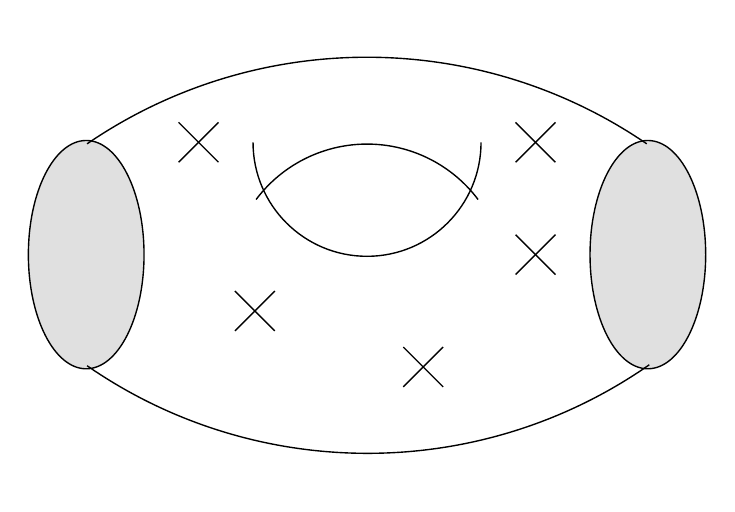
\begin{tikzpicture}[x=1pt,y=1pt,scale=1.10,transform shape,>=stealth,line width=0.5pt]
  \def\cr#1#2{\draw (#1-6.55,#2-6.55) -- (#1+6.55,#2+6.55);
               \draw (#1-6.55,#2+6.55) -- (#1+6.55,#2-6.55);}
  % ---- the two ends of the surface ----
  \draw[fill=black!12] (25.1,85.5) ellipse[x radius=19pt,y radius=37.5pt];
  \draw[fill=black!12] (209.6,85.5) ellipse[x radius=19pt,y radius=37.5pt];
  % ---- upper and lower boundary ----
  \draw (25.4,121.9) arc[start angle=124.4,end angle=55.6,radius=162.7pt];
  \draw (25.4,49.0) arc[start angle=235.3,end angle=304.9,radius=161.8pt];
  % ---- the cycle drawn on the surface ----
  \draw (80.9,103.6) arc[start angle=143.1,end angle=36.9,radius=45.6pt];
  \draw (79.9,122.4) arc[start angle=180,end angle=360,radius=37.45pt];
  % ---- punctures ----
  \cr{62.0}{122.4}
  \cr{172.7}{122.4}
  \cr{172.7}{85.5}
  \cr{80.5}{67.0}
  \cr{135.8}{48.6}
\end{tikzpicture}

\caption{带有一串正则奇点与非正则奇点的黎曼面；相应的四维理论是一个渐近自由理论，它由把 type IV Argyres--Douglas 理论与三孔球构成的 SCFT 规范化得到。}
\label{fig:11}
\end{figure}


% =====================================================================
%  sections/sec6.tex —— 6 由六维 A_{k-1} 理论得到的 AD 点（原文 pp.31–46）
% =====================================================================
\section{由六维 $A_{k-1}$ 理论得到的 AD 点}
\label{sec:ak}

\subsection{非正则奇点的选取}
\label{sec:6.1}

\routenote{原文 pp.31--33。本小节走反证：设奇点有两个 block、第二个 block 的维数 $k_2>1$，用「高阶极点的参数只能充当耦合常数与质量」定出最小算子的维数 $[v]$；再由 $[v]\le 1$ 与斜率顺序冲突，把这一类排除。剩下的只有两个 block 且 $k_2=1$，由此得到 Type I、Type II、Type III 三类奇点。}

现在从六维 $A_{n-1}$ 理论出发，把它紧致化在带非正则奇点的黎曼面上。首先要弄清：定义四维 SCFT 究竟需要哪一类非正则奇点。非正则奇点个数的分析同上一节：球面上可以只有一个非正则奇点，也可以在南北两极各放一个，即一个非正则奇点加一个正则奇点。在 $A_1$、$A_2$ 的情形，各类非正则奇点都能定义四维 SCFT。秩更高的群则不同：并非每个非正则奇点都能定义四维 AD 理论。

关键在于：高阶极点的参数应当充当耦合常数。因此，若 Seiberg--Witten 曲线中的某个算子只由这些参数构成，它的标度维数就必须小于一；换言之，这些项不能含有 Higgs 场的正则项给出的部分。这个条件对可用于寻找 SCFT 的非正则奇点类型施加了很强的限制。

非正则奇点由一串斜率确定，用这串斜率可以画出牛顿多边形。斜率按 $\lambda_1>\lambda_2>\cdots>\lambda_l$ 排列，其中 $\lambda_i=r_i-2$，$r_i$ 是非正则奇点中第 $i$ 个 block 的最大极点阶。先取 $\lambda_1=n_1+j_1/k_1$，其中 $j_1<k_2$、$n_1\ge 2$；这个 block 的领头阶矩阵取如下形式（奇点放在 $z=\infty$）：
\begin{equation}
B_1 = z^{n_1-2+j_1/k_1}\diag(1,\ \omega,\ \cdots,\ \omega^{k_1-1}) .
\label{eq:6.1}\tag{6.1}
\end{equation}
\typo{原文 p.32 的条件 $j_1<k_2$ 与 (3.15) 的 $0<j_i\le k_i$ 不协调。此处限定的是第一个 block 的分数部分，应为 $j_1<k_1$。}

这个 block 决定了各算子的标度维数，奇点处的 Seiberg--Witten 曲线为
\begin{equation}
x^n + x^{n-k_1}z^{k_1n_1-2k_1+j_1} = 0 ,
\label{eq:6.2}\tag{6.2}
\end{equation}
于是 $z$ 与 $x$ 的标度维数为
\begin{equation}
[z] = \frac{k_1}{k_1n_1-k_1+j_1},\qquad
[x] = \frac{k_1n_1-2k_1+j_1}{k_1n_1-k_1+j_1} .
\label{eq:6.3}\tag{6.3}
\end{equation}
\typo{原文 p.32 的 (6.2) 与 (6.4) 写作 $x^n$，这里的指数实为规范群的秩；原文从第 \ref{sec:6.1.1} 小节起改用 $k$。同样的滑移还见于 p.31 开头的「六维 $A_{n-1}$ 理论」——本节标题与后文都用 $A_{k-1}$。译文照录。}

现在打开第二个 block 对应的形变。该 block 的维数为 $k_2>1$，极点阶为 $r_2=n_1+j_2/k_2<r_1$（取 $n_2=n_1$，使 $[v]$ 的标度维数尽可能小），且 $j_2/k_2<j_1/k_1$。SW 曲线形如
\begin{equation}
\begin{aligned}
x^n &+ x^{n-k_1}z^{k_1n_1-2k_1+j_1}
+ x^{n-(k_1+k_2)}z^{k_1n_1-2k_1+j_1}\\
&\times\bigl(z^{k_2n_1-2k_2+j_2}+\cdots+vz^{(k_2-1)(n_1-2)+j_2-1}+\cdots\bigr) = 0 .
\end{aligned}
\label{eq:6.4}\tag{6.4}
\end{equation}
这里 $v$ 是只由高阶极点系数构成的最小算子，把谱曲线显式展开即可看出；它的标度维数由式 (6.3) 定出：
\begin{equation}
[v] = k_2[x]-\bigl((k_2-1)(n_1-2)+j_2-1\bigr)[z]
= \frac{(n_1-1)k_1+k_2j_1-k_1j_2}{k_1n_1-k_1+j_1} .
\label{eq:6.5}\tag{6.5}
\end{equation}
这个算子维数不得大于一，因为它必须充当耦合常数或质量。于是
\begin{equation}
[v]\le 1 \ \to\ k_2j_1-k_1j_2\le j_1
\ \to\ \frac{j_1}{k_1}\le\frac{j_2}{k_2-1}
\ \to\ \frac{j_1}{k_1}<\frac{j_2}{k_2} .
\label{eq:6.6}\tag{6.6}
\end{equation}
这与假设 $j_1/k_1>j_2/k_2$ 矛盾。

\zhnote{[译者按（无外部依据）：(6.6) 的末一步推不出来。当 $k_2>1$ 时总有 $j_2/(k_2-1)>j_2/k_2$，所以 $j_1/k_1\le j_2/(k_2-1)$ 并不能与 $j_1/k_1>j_2/k_2$ 冲突。原文此处的矛盾论证有缺口，下文结论照录原文。]}

\begin{figure}[tbp]
\centering
% Figure 12 -- graphic form of the Seiberg-Witten curve
\begin{tikzpicture}[x=1pt,y=1pt,scale=1.08,transform shape,>=stealth,line width=0.5pt]
  % ---- axes ----
  \draw (52.4,8.6) -- (52.4,175.3);
  \draw (4.6,56.4) -- (230.5,56.4);
  % ---- Newton-polygon-like outline ----
  \draw (99.6,56.0) -- (99.6,139.7) -- (147.5,115.5) -- (147.2,56.0);
  \draw (147.5,115.5) -- (206.7,56.2);
  % ---- k1, k2 brackets ----
  \draw (99.4,50.3) -- (117.9,50.4) -- (123.7,44.1) -- (129.7,50.6) -- (141.6,50.3);
  \draw (146.8,50.3) -- (171.3,50.4) -- (177.1,44.1) -- (183.0,50.6) -- (206.8,50.3);
  % ---- h1, h2 markers ----
  \draw (93.9,91.6) -- (81.9,139.8);
  \draw (93.9,92.3) -- (82.0,62.0);
  \draw (141.3,116.0) -- (135.3,85.7);
  \draw (141.3,62.0) -- (135.2,86.4);
  % ---- distinguished points ----
  \fill (82.0,145.3) circle[radius=1.85pt];
  \fill (70.1,151.2) circle[radius=1.85pt];
  % ---- labels ----
  \node[inner sep=0pt] at (181.25,35.6) {\fontsize{9}{11}\selectfont$k_1$};
  \node[inner sep=0pt] at (121.95,35.6) {\fontsize{9}{11}\selectfont$k_2$};
  \node[inner sep=0pt] at (127.95,88.9) {\fontsize{9}{11}\selectfont$h_1$};
  \node[inner sep=0pt] at (74.55,94.85) {\fontsize{9}{11}\selectfont$h_2$};
\end{tikzpicture}

\caption{由非正则奇点定义的 SW 曲线的图形。该奇点的领头阶矩阵含大小为 $k_1$、$k_2$、… 的 block。}
\label{fig:12}
\end{figure}

剩下的唯一可能是只有两个 block，且 $k_2=1$。此时领头阶矩阵为
\begin{equation}
\Phi = z^{n+\frac{j}{k-1}-2}\diag(0,\ 1,\ \omega,\ \cdots,\ \omega^{(k-1)-1}) .
\label{eq:6.7}\tag{6.7}
\end{equation}
因此，可用于定义 AD 理论的非正则奇点分类如下：
\begin{enumerate}
  \item Type I 奇点：
\begin{equation}
\Phi = z^{n+\frac{j}{k}-2}\diag(1,\ \omega,\ \cdots,\ \omega^{n-1}),\qquad 0<j\le k .
\label{eq:6.8}\tag{6.8}
\end{equation}
  \item Type II 奇点：
\begin{equation}
\Phi = z^{n+\frac{j}{k-1}-2}\diag(0,\ 1,\ \omega,\ \cdots,\ \omega^{(n-1)-1}),\qquad 0<j<k-1 .
\label{eq:6.9}\tag{6.9}
\end{equation}
\typo{原文 p.33 的 (6.8) 把对角元写到 $\omega^{n-1}$，应为 $\omega^{k-1}$；(6.9) 写到 $\omega^{(n-1)-1}$，应为 $\omega^{(k-1)-1}$，依据是 (6.7) 的同型写法 $\omega^{(k-1)-1}$。矩阵的阶由规范群秩 $k$ 定，与极点阶的整数部分 $n$ 无关。}
  \item Type III 奇点：可以考虑上述非正则奇点的退化。有两种情形。

  \textbf{Case 1：}极点阶为整数。此时奇点由一列杨图 $Y_n\subseteq Y_{n-1}\cdots\subseteq Y_1$ 指定，其中 $Y_{j-1}$ 由 $Y_j$ 的每一列进一步分拆得到。

  \textbf{Case 2：}极点阶为分数。此时只需确定分拆，它由牛顿多边形上的整点定出。例如，若一般的奇点为
\begin{equation}
\Phi = z^{n-2+\frac{2}{4}}\diag(1,\ \omega,\ \cdots,\ \omega^{3}) ,
\label{eq:6.10}\tag{6.10}
\end{equation}
牛顿多边形的边界上就会出现一个整点。若选取这个点，领头阶奇点可退化为
\begin{equation}
A_0 = z^{n-2+\frac{2}{4}}\diag(1,\ -1,\ 1,\ -1) .
\label{eq:6.11}\tag{6.11}
\end{equation}
\zhnote{[依据：(6.10) 与 (6.11) 的对照。] (6.11) 中的 $A_0$ 是退化后领头阶矩阵的名字，并不是一个叫 $A_0$ 的理论，与六维 $A_{n-1}$ 理论的 $A$ 记号无关。}
\end{enumerate}

下面略谈应与物理考虑相匹配的几何量。例如，库仑分支的维数应与 Hitchin 纤维化的底的维数相等，即 Hitchin 模空间维数的一半。质量参数则基本由一阶极点系数的形式定出。

以上列表穷尽了可用于定义 SCFT 的全部非正则奇点。下面逐一细看。

\subsubsection{Type I SCFT：$(A_{k-1},A_{N-1})$ 理论}
\label{sec:6.1.1}

把六维 $A_{k-1}$ 理论紧致化到带 Type I 非正则奇点的球面上。只打开领头阶矩阵时，奇点处四维 SCFT 的 Seiberg--Witten 曲线为
\begin{equation}
x^k+z^N = 0 .
\label{eq:6.12}\tag{6.12}
\end{equation}
这个奇点的极点阶为 $r=N/k+2$，并用标度不变性把 $z^N$ 的系数定为 1。$x$ 与 $z$ 的标度维数为
\begin{equation}
[x] = \frac{N}{N+k},\qquad [z] = \frac{k}{N+k} .
\label{eq:6.13}\tag{6.13}
\end{equation}
文献 \cite{17} 把这个理论称为 $(A_{k-1},A_{N-1})$ 理论，因为它的 BPS 箭图是相应类型两个 Dynkin 图的乘积。一般形变下的 Seiberg--Witten 曲线很好写：只需取相应非正则奇点的牛顿多边形所围的整点，坐标为 $(m,n)$ 的每个整点对应一个形变项 $x^mz^n$。$x=k-1$ 线上的点不用，因为规范群是 $\SU(k)$。$z=N-1$ 线上的点也全部去掉。多数情形下，这条线上牛顿多边形所围的整点只有一个，用平移不变性即可去掉。另一些情形下，这些额外的形变对这个 SCFT 不允许，但对后文由再加一个正则奇点得到的 SCFT 却是必需的。图 \ref{fig:13} 给出几个例子，它们都由六维 $A_3$ 理论得到。

例如，按上述规则，$(A_3,A_2)$ 理论的 Seiberg--Witten 曲线为
\begin{equation}
x^4+(v_1z+v_2)x^2+(v_3z+v_4)x+z^3+v_5z+v_6 = 0 .
\label{eq:6.14}\tag{6.14}
\end{equation}
由此容易求出各算子的标度维数，并显式验证每个相关算子都有耦合常数与之配对。

相关算子与耦合常数之间的配对，在一般情形下也能证明。先看 $x=k-2$ 线上的点。这条线上的形变为 $u_ix^{k-2}z^i$，$u_i$ 的标度维数为
\begin{equation}
[u_i] = 2[x]-i[z] .
\label{eq:6.15}\tag{6.15}
\end{equation}
只要上述标度维数为正，任何非负整数 $i$ 都允许。再看 $x=0$ 线上的形变，其形式为 $v_jz^{N-j}$，$2\le j\le N$；$v_j$ 的标度维数为
\begin{equation}
[v_j] = j[z] .
\label{eq:6.16}\tag{6.16}
\end{equation}

两族算子的维数之和为
\begin{equation}
[u_i]+[v_j] = 2[x]+(j-i)[z] .
\label{eq:6.17}\tag{6.17}
\end{equation}
利用条件 $2[x]+2[z]=2$，取 $j-i=2$ 即知这两条线上的所有相关算子都有配对。类似的分析适用于 $x=k-2-l$ 与 $x=l$ 线上的形变。注意，去掉 $z=N-1$ 线上的算子对配对至关重要。

\begin{figure}[tbp]
\centering
% Figure 13 -- Seiberg-Witten graphs for (A3,A2), (A3,A3), (A3,A4)
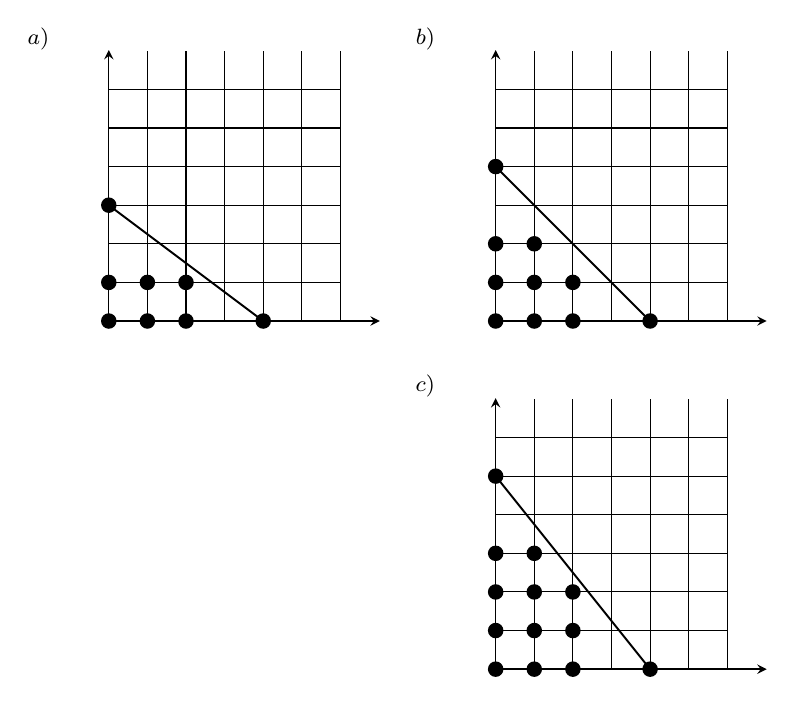
\begin{tikzpicture}[x=1pt,y=1pt,>=stealth,line width=0.5pt]
  \def\u{13.95}
  % ================= panel a) =================
  \begin{scope}[xshift=48.3pt,yshift=134.5pt]
    \draw[line width=0.4pt] \foreach \i in {1,...,6} {(\i*\u,0) -- (\i*\u,{7*\u})};
    \draw[line width=0.4pt] \foreach \j in {1,...,6} {(0,\j*\u) -- ({6*\u},\j*\u)};
    \draw[->] (0,0) -- (0,{7.02*\u});
    \draw[->] (0,0) -- ({7.02*\u},0);
    \draw[line width=0.7pt] (0,{3*\u}) -- ({4*\u},0);
    \foreach \i/\j in {0/0,1/0,2/0,4/0,0/1,1/1,2/1,0/3}
      {\fill ({\i*\u},{\j*\u}) circle[radius=2.8pt];}
  \end{scope}
  % ================= panel b) =================
  \begin{scope}[xshift=188.1pt,yshift=134.5pt]
    \draw[line width=0.4pt] \foreach \i in {1,...,6} {(\i*\u,0) -- (\i*\u,{7*\u})};
    \draw[line width=0.4pt] \foreach \j in {1,...,6} {(0,\j*\u) -- ({6*\u},\j*\u)};
    \draw[->] (0,0) -- (0,{7.02*\u});
    \draw[->] (0,0) -- ({7.02*\u},0);
    \draw[line width=0.7pt] (0,{4*\u}) -- ({4*\u},0);
    \foreach \i/\j in {0/0,1/0,2/0,4/0,0/1,1/1,2/1,0/2,1/2,0/4}
      {\fill ({\i*\u},{\j*\u}) circle[radius=2.8pt];}
  \end{scope}
  % ================= panel c) =================
  \begin{scope}[xshift=188.1pt,yshift=8.7pt]
    \draw[line width=0.4pt] \foreach \i in {1,...,6} {(\i*\u,0) -- (\i*\u,{7*\u})};
    \draw[line width=0.4pt] \foreach \j in {1,...,6} {(0,\j*\u) -- ({6*\u},\j*\u)};
    \draw[->] (0,0) -- (0,{7.02*\u});
    \draw[->] (0,0) -- ({7.02*\u},0);
    \draw[line width=0.7pt] (0,{5*\u}) -- ({4*\u},0);
    \foreach \i/\j in {0/0,1/0,2/0,4/0,0/1,1/1,2/1,0/2,1/2,2/2,0/3,1/3,0/5}
      {\fill ({\i*\u},{\j*\u}) circle[radius=2.8pt];}
  \end{scope}
  % ================= panel labels =================
  \node[inner sep=0pt] at (22.9,236.5) {\fontsize{8}{10}\selectfont$a)$};
  \node[inner sep=0pt] at (162.7,236.5) {\fontsize{8}{10}\selectfont$b)$};
  \node[inner sep=0pt] at (162.7,111.1) {\fontsize{8}{10}\selectfont$c)$};
\end{tikzpicture}

\caption{a）$(A_3,A_2)$ 理论的 Seiberg--Witten 图；b）$(A_3,A_3)$ 理论的 Seiberg--Witten 图；c）$(A_3,A_4)$ 理论的 Seiberg--Witten 图。}
\label{fig:13}
\end{figure}

若相应的非正则奇点具有整数极点，则领头阶系数中还有 $N-2$ 个可以打开的额外参数。这些参数无量纲；幸运的是，谱中确实有 $N-2$ 个维数为二的算子，于是这些无量纲耦合常数自然地与严格边缘（exactly marginal）形变等同起来。与熟悉的 $\sN{=}4$ SYM 理论不同，这些 AD 理论在共形流形上似乎没有弱耦合描述。

有趣的是，把 $x$ 轴与 $y$ 轴互换，算子谱完全相同；因此 $(A_{k-1},A_{N-1})$ 理论与 $(A_{N-1},A_{k-1})$ 理论等价。显式数出库仑分支形变的个数与质量参数的个数，即可证明 $(A_{N-1},A_{k-1})$ 理论电荷格的秩为
\begin{equation}
R = 2n_c+n_f = (k-1)(N-1) .
\label{eq:6.18}\tag{6.18}
\end{equation}
这与 BPS 箭图中箭图节点的个数一致，正如其名字所提示的。

上述事实可用非正则奇点的几何性质来核对。设奇点具有整数极点，阶为 $r=nk/k+2=n+2$，它实际上定义了 $(A_{k-1},A_{nk-1})$ 理论。带这种非正则奇点的模空间维数为
\begin{equation}
d = (n+2)(k^2-k)-2(k^2-1) = (nk-1)(k-1)-(k-1) .
\label{eq:6.19}\tag{6.19}
\end{equation}
这个数等于 $2n_r$，其中 $n_r$ 是库仑分支一般点处规范群的秩；此外还有 $n_f=k-1$ 个质量参数。于是由几何考虑得到电荷格的秩为
\begin{equation}
R = (k-1)(nk-1) ,
\label{eq:6.20}\tag{6.20}
\end{equation}

\subsubsection{Type II SCFT}
\label{sec:6.1.2}

这类 SCFT 由球面上的 type II 非正则奇点定义，SCFT 点处的 Seiberg--Witten 曲线为
\begin{equation}
x^k+z^Nx = 0 ,
\label{eq:6.21}\tag{6.21}
\end{equation}
于是坐标 $x$ 与 $z$ 的标度维数为
\begin{equation}
[x] = \frac{N}{k-1+N},\qquad [z] = \frac{k-1}{k-1+N} .
\label{eq:6.22}\tag{6.22}
\end{equation}
该非正则奇点的极点阶为 $r=N/(k-1)+2$。同样，理论的一般形变完全由相应非正则奇点的牛顿多边形定出。例子见图 \ref{fig:14}。大小为 $k-1$ 的那个 block 与 $(A_{k-2},A_{N-1})$ 理论相同，这一部分的谱分析与 Type I 理论相同。还可以验证，额外的 $x=0$ 线上每个相关算子都有耦合常数与之配对。

\begin{figure}[tbp]
\centering
% Figure 14 -- the Seiberg-Witten curve from the marked integer points
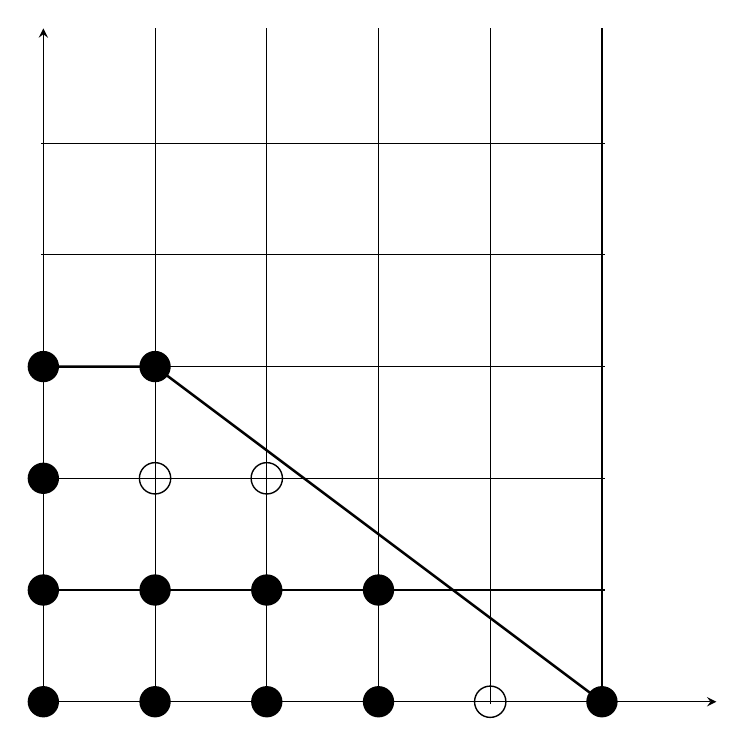
\begin{tikzpicture}[x=1pt,y=1pt,scale=1.08,transform shape,>=stealth,line width=0.5pt]
  \def\u{37.38}
  % ---- grid ----
  \foreach \i in {1,...,5} {\draw[line width=0.4pt] ({24.1+\i*\u},33.5) -- ({24.1+\i*\u},259.6);}
  \foreach \j in {1,...,5} {\draw[line width=0.4pt] (23.4,{34.3+\j*\u}) -- (211.96,{34.3+\j*\u});}
  % ---- axes ----
  \draw[->] (23.4,34.3) -- (249.3,34.3);
  \draw[->] (24.1,33.5) -- (24.1,259.6);
  % ---- Newton polygon ----
  \draw[line width=0.9pt] (24.1,{34.3+3*\u}) -- ({24.1+\u},{34.3+3*\u}) -- ({24.1+5*\u},34.3);
  % ---- marked lattice points ----
  \foreach \i/\j in {0/0,1/0,2/0,3/0,5/0,0/1,1/1,2/1,3/1,0/2,0/3,1/3}
    {\fill ({24.1+\i*\u},{34.3+\j*\u}) circle[radius=5.24pt];}
  \foreach \i/\j in {4/0,1/2,2/2}
    {\draw ({24.1+\i*\u},{34.3+\j*\u}) circle[radius=5.24pt];}
\end{tikzpicture}

\caption{由牛顿多边形所围的带标记整点读出 Seiberg--Witten 曲线。}
\label{fig:14}
\end{figure}

\subsubsection{Type III SCFT}
\label{sec:6.1.3}

用 type III 非正则奇点定义的 SCFT 稍难分析。先看整数极点的情形。此时奇点由一列杨图 $Y_n\subseteq Y_{n-1}\cdots\subseteq Y_1$ 指定，其中 $n=N/k+2$。奇点处的 Seiberg--Witten 曲线为
\begin{equation}
x^k+u_1x^{N-2}+u_2x^{N-3}+\cdots+z^N = 0 ,
\label{eq:6.23}\tag{6.23}
\end{equation}
其中 $u_i$ 经过调节，使根具有 $Y_n$ 所定的退化。形变后的 Seiberg--Witten 曲线与未退化时相同；但并非所有算子都独立，它们之间满足相当复杂的关系。我们想知道谱的标度维数。与正则穿刺点的情形一样，这些信息包含在相应的杨图序列里。一般的 Seiberg--Witten 曲线为
\begin{equation}
x^k+\sum_{i=2}^{k}\Phi_i(z)z^{k-i} = 0 .
\label{eq:6.24}\tag{6.24}
\end{equation}
$\Phi_i$ 中系数为库仑分支算子的 $z$ 最高幂次，由下述数据定出：
\begin{equation}
m_i = \sum_j p_i^{(j)}-2i+1 ,
\label{eq:6.25}\tag{6.25}
\end{equation}
其中 $p_i^{(j)}=i-s_i$，$s_i$ 是第 $j$ 个杨图中第 $i$ 个格子的高度；$\Phi_i$ 具有如下形式
\begin{equation}
\Phi_i = \cdots+u_1z^{m_i-1}+u_2z^{m_i-2}+\cdots+c ,
\label{eq:6.26}\tag{6.26}
\end{equation}
标号为 $u_1$、$u_2$、…、$c$ 的系数就是独立的库仑分支算子。
\typo{原文 p.37 的 (6.25) 与 (5.18) 的 $d_i=\sum_j p_i^{(j)}-2i$ 相差一。两者数的对象不同：(5.18) 数的是第 $i$ 个微分的极点阶，这里数的是 $\Phi_i$ 中库仑分支算子所占的最高 $z$ 幂次，后者比极点阶多一项。两式并不矛盾。}

有两个特例值得再谈，用正则穿刺点定义理论时也会遇到同样情形。第一种是领头阶系数中的数 $m_k$ 为零或负；此时不能再用上述办法求谱，目前我们也找不到系统处理它的方法。另一种是 $m_k$ 非零，但有些别的 $m_j$ 为负；此时仍可用上面的计算求谱，但库仑分支的维数与 Hitchin 纤维化的底的维数不再相等。

若极点阶为分数，可用类似方法求出退化情形的谱。这留给感兴趣的读者。

这些位形并不总能定义 SCFT，因为无量纲耦合（编码在非正则奇点的领头阶矩阵里）与维数为二的算子之间可能没有配对。判断何时才能成为 SCFT，留待以后研究。

\subsubsection{再加一个正则奇点：Type IV SCFT}
\label{sec:6.1.4}

可以在上述情形上再加一个正则奇点，并在红外找到 AD 理论。图 \ref{fig:15} 给出一个例子。注意，这里把非正则奇点所有可能的形变都打开，好让来自正则奇点的相关形变能有耦合常数与之配对。于是先前不允许的那些耦合常数在此起了重要作用。

计算 Seiberg--Witten 曲线时，用到正则穿刺点杨图 $Y_0$ 中的数据。例如，由正则奇点带来的独立库仑分支参数在 Seiberg--Witten 曲线中具有如下形式
\begin{equation}
\Phi_i = \cdots+\bigl(v_1z^{-1}+\cdots+v_{n_i}z^{-n_i}\bigr) ,
\label{eq:6.27}\tag{6.27}
\end{equation}
这里 $\Phi_i$ 是 $i$ 次微分；$n_i=i-s_i$，其中 $s_i$ 是杨图 $Y_0$ 中第 $i$ 个格子的高度。
\typo{原文 p.38 在此处措辞自我重复（「$i$ the $i$th box」与「$s_i$ the height of the $i$th box」连用），译文按「$s_i$ 是第 $i$ 个格子的高度」处理。}

\begin{figure}[tbp]
\centering
% Figure 15 -- Seiberg-Witten graph for an irregular + a regular singularity
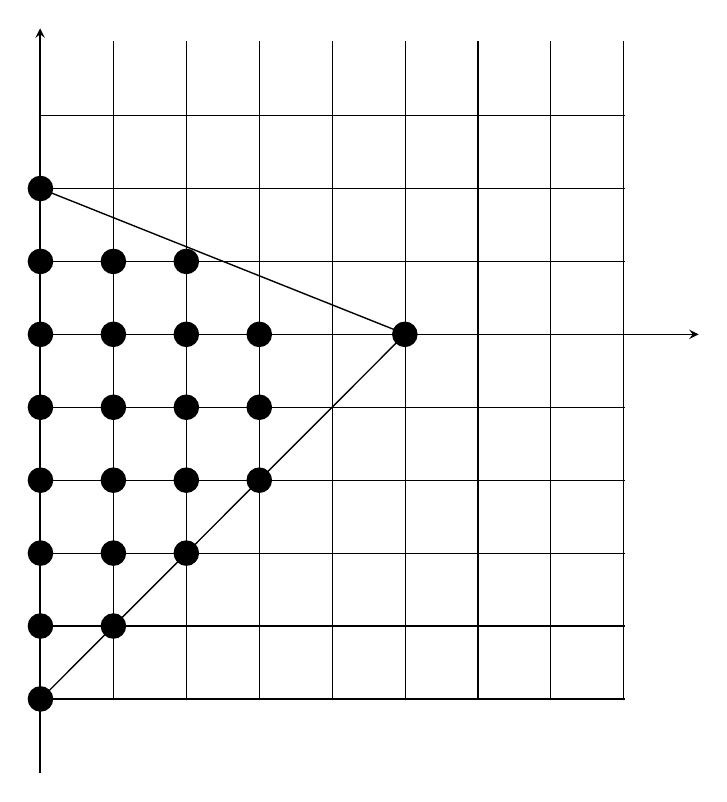
\begin{tikzpicture}[x=1pt,y=1pt,scale=1.05,transform shape,>=stealth,line width=0.5pt]
  \def\u{25.095}
  % ---- grid ----
  \foreach \i in {0,...,8} {\draw[line width=0.4pt] (66.5,28.4) ++(\i*\u,0) -- ++(0,227.1);}
  \foreach \j in {-5,...,3} {\draw[line width=0.4pt] (65.9,{154.4+\j*\u}) -- (267.8,{154.4+\j*\u});}
  % ---- axes ----
  \draw[->] (65.9,154.4) -- (293,154.4);
  \draw[->] (66.4,3.4) -- (66.4,259.7);
  % ---- the two Newton-polygon edges ----
  \draw (66.6,28.9) -- (191.9,154.4);
  \draw (65.9,204.8) -- (192.6,154.3);
  % ---- marked points ----
  \foreach \j in {2,1,0,-1,-2,-3,-4,-5} {\fill (66.5,{154.4+\j*\u}) circle[radius=4.4pt];}
  \foreach \j in {1,0,-1,-2,-3,-4}     {\fill (91.6,{154.4+\j*\u}) circle[radius=4.4pt];}
  \foreach \j in {1,0,-1,-2,-3}        {\fill (116.7,{154.4+\j*\u}) circle[radius=4.4pt];}
  \foreach \j in {0,-1,-2}             {\fill (141.8,{154.4+\j*\u}) circle[radius=4.4pt];}
  \fill (191.9,154.4) circle[radius=4.4pt];
\end{tikzpicture}

\caption{带一个非正则奇点与一个正则奇点的理论的 Seiberg--Witten 图。}
\label{fig:15}
\end{figure}

正则穿刺点可以带有非阿贝尔味对称性，这类 SCFT 在构造渐近自由理论时很重要。在球上放多个非正则奇点所定义的理论里，它们会自然出现：相应的四维理论是把这些 AD 理论一起规范化得到的渐近自由理论，而非正则奇点总位于退化极限下的边界上。

\subsection{三维镜像对称}
\label{sec:6.2}

三维镜像理论同样可以通过寻找接在非正则奇点上的箭图得到。目前只知道整数极点非正则奇点所定义的理论的三维镜像；这类奇点由一列杨图 $Y_n\subseteq Y_{n-1}\cdots\subseteq Y_1$ 分类，其中 $Y_j$ 由 $Y_{j+1}$ 的每一列进一步分拆得到。相应的数学考虑见文献 \cite{39}，其结果的解释正是 Argyres--Douglas 理论的三维镜像对称。

\routenote{原文 pp.38--39。镜像箭图分三步造出。先把 $Y_n$ 的每一列变成一个节点，节点之间按极点阶的整数部分放箭；再沿 $Y_{n-1},\dots,Y_2$ 逐层细分节点；最后把 $Y_1$ 这一层换成正则奇点处早已熟悉的箭图支链。三步拼起来，箭图节点的总秩恰为 $k$。}

三维镜像理论按如下步骤逐步构造。设 $Y_n$ 的分拆为 $[n_1,n_2,\dots,n_r]$，第一步的箭图有 $r$ 个节点，每个节点的秩为 $n_i$，即 $U(n_i)$ 的秩；各节点之间还有 $n-2$ 支箭，代表双基本表示，第一步见图 \ref{fig:16}。第二步：设 $Y_1$ 中某个 $n_i$ 在杨图 $Y_{n-1}$ 中进一步分拆为 $[m_{i1},m_{i2},\dots,m_{is}]$。于是把第一步中秩为 $n_i$ 的箭图节点分裂为 $s$ 个箭图节点，新节点的秩由分拆 $m_{ij}$ 定出，这些新节点之间放 $n-3$ 支箭。此外，分裂出的节点与其他簇中的节点之间仍保留 $n-2$ 支箭，见图 \ref{fig:16}。对每个杨图都做同样的分裂，直到 $Y_2$，就得到由若干节点与箭组成的箭图。注意，所有箭图节点的秩之和为 $k$。

\typo{原文 p.39 此句写「设 $Y_1$ 中某个 $n_i$ 在杨图 $Y_{n-1}$ 中进一步分拆为」。第一步分拆的对象是 $Y_n$，而 $Y_{n-1}$ 是把 $Y_n$ 的每一列进一步分拆得到的（见 Case 1 的定义），故这里应为 $Y_n$；$Y_1$ 是这条链的最后一项，对应质量矩阵，下一段才用到。译文照录原文的 $Y_1$。}

$Y_1$ 即质量矩阵这一层需要特殊处理：若 $Y_2$ 的某一列高为 $l$，而它在 $Y_1$ 中进一步分拆为 $[l_1,l_2,\dots,l_t]$，则不按上述方式分解这个节点，而是像正则奇点那样接一条箭图支链（quiver leg/tail），其总格数为 $l$ \cite{38}。具体地说，定义 $h_i=\sum_{j=t-i+1}^{t}l_j$，这一部分的箭图支链见图 \ref{fig:16}。

若另有一个由杨图指定的正则奇点，则先按图 \ref{fig:16} 底部所示接一条箭图支链，总格数为 $k$。然后把 $U(k)$ 节点按非正则奇点的杨图 $Y_2$ 所定的模式 spray。最后把两个箭图粘合起来，做法是把正则奇点支链上经 spray 得到的节点与非正则奇点箭图中的节点认同。

\begin{figure}[tbp]
\centering
% Figure 16 -- step 1 / step 2 quivers and the quiver tail of the regular singularity
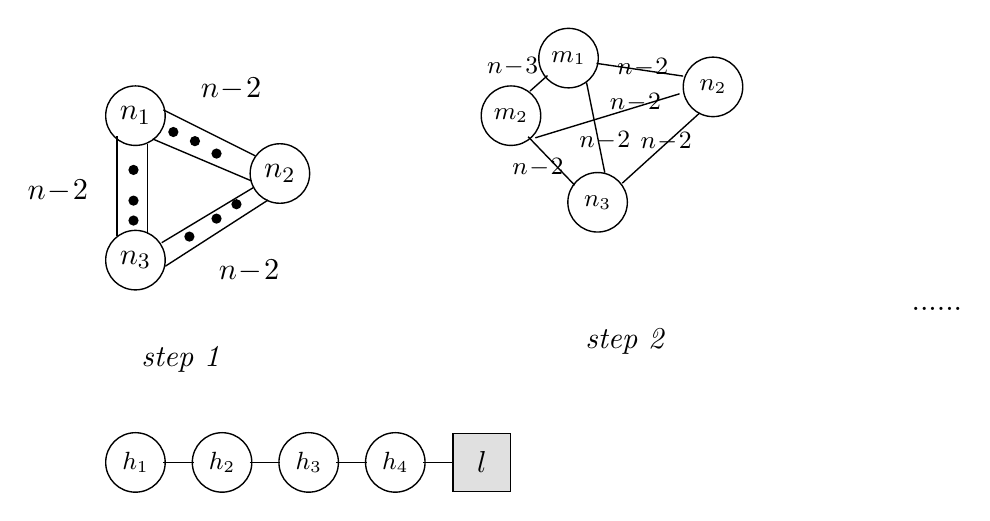
\begin{tikzpicture}[x=1pt,y=1pt,>=stealth,line width=0.5pt,
   circ/.style={circle,draw,minimum size=21.5pt,inner sep=0pt}]
  \def\rr{1.85}
  % ======================== step 1 ========================
  % --- n1--n3 ribbon ---
  \draw (50.1,104.0) -- (50.1,140.1);
  \draw (61.2,105.0) -- (61.2,137.5);
  \foreach \y in {384.0,395.1,402.3} {\fill (56.1,{512-\y}) circle[radius=\rr pt];}
  % --- n1--n2 ribbon ---
  \draw (63.0,139.2) -- (98.8,124.0);
  \draw (66.9,149.7) -- (100.1,133.1);
  \fill (70.5,141.7) circle[radius=\rr pt];
  \fill (78.3,138.4) circle[radius=\rr pt];
  \fill (86.1,133.9) circle[radius=\rr pt];
  % --- n3--n2 ribbon ---
  \draw (66.3,101.7) -- (99.4,121.6);
  \draw (67.6,93.2) -- (104.7,117.1);
  \fill (76.3,103.9) circle[radius=\rr pt];
  \fill (86.1,110.4) circle[radius=\rr pt];
  \fill (93.3,115.6) circle[radius=\rr pt];
  % ======================== step 2 ========================
  \draw (199.4,156.5) -- (205.7,162.1);
  \draw (223.4,166.5) -- (254.7,161.9);
  \draw (219.8,159.6) -- (226.4,127.0);
  \draw (198.7,140.0) -- (215.5,122.5);
  \draw (201.3,139.6) -- (253.4,155.5);
  \draw (232.7,123.2) -- (260.5,148.4);
  % ======================== nodes ========================
  \node[circ] (n1) at (56.8,147.6)   {\fontsize{11}{13}\selectfont$n_1$};
  \node[circ] (n2) at (109.0,126.7)  {\fontsize{11}{13}\selectfont$n_2$};
  \node[circ] (n3) at (56.8,95.4)    {\fontsize{11}{13}\selectfont$n_3$};
  \node[circ] (mm1) at (213.3,168.4) {\fontsize{9}{11}\selectfont$m_1$};
  \node[circ] (mm2) at (192.5,147.6) {\fontsize{9}{11}\selectfont$m_2$};
  \node[circ] (sn3) at (223.8,116.3) {\fontsize{9}{11}\selectfont$n_3$};
  \node[circ] (sn2) at (265.5,158.0) {\fontsize{9}{11}\selectfont$n_2$};
  % ======================== quiver tail ========================
  \draw (66.8,22.3) -- (77.9,22.3);
  \draw (98.1,22.3) -- (109.2,22.3);
  \draw (129.4,22.3) -- (140.5,22.3);
  \draw (160.8,22.3) -- (171.6,22.3);
  \draw[fill=black!12] (171.6,11.9) rectangle (192.4,32.8);
  \node[circ] (h1) at (56.8,22.3)  {\fontsize{9}{11}\selectfont$h_1$};
  \node[circ] (h2) at (88.1,22.3)  {\fontsize{9}{11}\selectfont$h_2$};
  \node[circ] (h3) at (119.4,22.3) {\fontsize{9}{11}\selectfont$h_3$};
  \node[circ] (h4) at (150.7,22.3) {\fontsize{9}{11}\selectfont$h_4$};
  \node[inner sep=0pt] at (182.0,22.35) {\fontsize{11}{13}\selectfont$l$};
  % ======================== labels ========================
  \node[inner sep=0pt] at (91.35,157.35) {\fontsize{11}{13}\selectfont$n\!-\!2$};
  \node[inner sep=0pt] at (97.85,91.55)  {\fontsize{11}{13}\selectfont$n\!-\!2$};
  \node[inner sep=0pt] at (28.75,120.25) {\fontsize{11}{13}\selectfont$n\!-\!2$};
  \node[inner sep=0pt] at (193.1,165.5)  {\fontsize{9}{11}\selectfont$n\!-\!3$};
  \node[inner sep=0pt] at (240.1,164.85) {\fontsize{9}{11}\selectfont$n\!-\!2$};
  \node[inner sep=0pt] at (237.45,152.45){\fontsize{9}{11}\selectfont$n\!-\!2$};
  \node[inner sep=0pt] at (226.4,138.75) {\fontsize{9}{11}\selectfont$n\!-\!2$};
  \node[inner sep=0pt] at (248.55,138.1) {\fontsize{9}{11}\selectfont$n\!-\!2$};
  \node[inner sep=0pt] at (202.25,129.0) {\fontsize{9}{11}\selectfont$n\!-\!2$};
  \node[inner sep=0pt] at (73.1,59.55)   {\fontsize{11}{13}\itshape step 1};
  \node[inner sep=0pt] at (233.55,66.05) {\fontsize{11}{13}\itshape step 2};
  \node[inner sep=0pt] at (346.4,77.85)  {\fontsize{11}{13}\selectfont......};
\end{tikzpicture}

\caption{第一步：若第一个杨图 $Y_n$ 的分拆为 $[n_1,n_2,n_3]$，则有一条含三个节点的箭图支链，各节点的秩为 $n_i$，这些节点之间有 $n-2$ 支箭。第二步：若 $n_1$ 在 $Y_{n-1}$ 中进一步分拆为 $[m_1,m_2]$，则把秩为 $n_1$ 的箭图节点分裂为两个箭图节点，秩分别为 $m_1$ 与 $m_2$；$m_i$ 与 $n_1$、$n_2$ 之间的箭不变，$m_1$ 与 $m_2$ 之间新添 $n-3$ 支箭。对其他杨图重复同样步骤，直到 $Y_2$ 为止。底部：若 $Y_2$ 中高为 $l$ 的列进一步分拆为 $[l_1,l_2,\dots,l_t]$，则在 $(Y_n,\dots,Y_2)$ 所定箭图中秩为 $l$ 的节点上接一条箭图支链。}
\label{fig:16}
\end{figure}

下面给出几个显例。

例 1：有一个极点阶为三的非正则奇点，其杨图为 $[2,2]$、$[1,1,1,1]$、$[1,1,1,1]$，箭图见图 \ref{fig:17}a。

例 2：有一个极点阶为四的非正则奇点，其杨图为 $[3,2]$、$[3,1,1]$、$[3,1,1]$、$[1,1,1,1,1]$，箭图见图 \ref{fig:17}b。

例 3：有一个极点阶为三的非正则奇点，其杨图为 $[1,1,1,1]$、$[1,1,1,1]$、$[1,1,1,1]$，另有一个满正则奇点，箭图见图 \ref{fig:17}c。

\begin{figure}[tbp]
\centering
% Figure 17 -- 3d mirrors for the AD theories of Examples 1, 2, 3
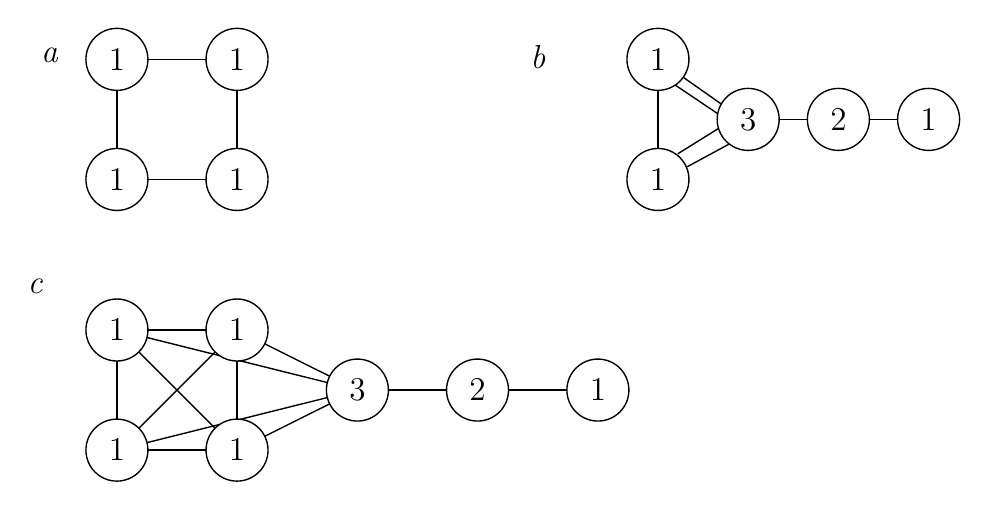
\begin{tikzpicture}[x=1pt,y=1pt,>=stealth,line width=0.5pt,
   nd/.style={circle,draw,fill=white,minimum size=22.4pt,inner sep=0pt}]
  % ===================== a) =====================
  \draw (37.6,164.0) rectangle (81.0,120.6);
  % ===================== b) =====================
  \draw (233.1,164.0) -- (233.1,120.6);
  \draw (238.3,155.4) -- (255.1,144.1);
  \draw (242.4,157.4) -- (256.5,147.5);
  \draw (240.3,129.9) -- (255.1,139.1);
  \draw (243.7,125.2) -- (259.2,133.6);
  \draw (265.7,142.3) -- (298.3,142.3) -- (330.9,142.3);
  % ===================== c) =====================
  \draw (37.6,66.2) -- (81.0,66.2) -- (81.0,22.8) -- (37.6,22.8) -- cycle;
  \draw (37.6,66.2) -- (81.0,22.8);
  \draw (37.6,22.8) -- (81.0,66.2);
  \draw (37.6,66.2) -- (124.5,44.5);
  \draw (81.0,66.2) -- (124.5,44.5);
  \draw (37.6,22.8) -- (124.5,44.5);
  \draw (81.0,22.8) -- (124.5,44.5);
  \draw (124.5,44.5) -- (167.9,44.5) -- (211.4,44.5);
  % ===================== nodes =====================
  \foreach \x/\y in {37.6/164.0,81.0/164.0,81.0/120.6,37.6/120.6}
    {\node[nd] at (\x,\y) {\fontsize{12}{14}\selectfont 1};}
  \foreach \x/\y in {233.1/164.0,233.1/120.6}
    {\node[nd] at (\x,\y) {\fontsize{12}{14}\selectfont 1};}
  \node[nd] at (265.7,142.3) {\fontsize{12}{14}\selectfont 3};
  \node[nd] at (298.3,142.3) {\fontsize{12}{14}\selectfont 2};
  \node[nd] at (330.9,142.3) {\fontsize{12}{14}\selectfont 1};
  \foreach \x/\y in {37.6/66.2,81.0/66.2,37.6/22.8,81.0/22.8}
    {\node[nd] at (\x,\y) {\fontsize{12}{14}\selectfont 1};}
  \node[nd] at (124.5,44.5) {\fontsize{12}{14}\selectfont 3};
  \node[nd] at (167.9,44.5) {\fontsize{12}{14}\selectfont 2};
  \node[nd] at (211.4,44.5) {\fontsize{12}{14}\selectfont 1};
  % ===================== panel letters =====================
  \node[inner sep=0pt] at (13.1,165.45) {\fontsize{12}{14}\itshape a};
  \node[inner sep=0pt] at (189.7,164.75) {\fontsize{12}{14}\itshape b};
  \node[inner sep=0pt] at (8.05,81.9)   {\fontsize{12}{14}\itshape c};
\end{tikzpicture}

\caption{例 1、例 2、例 3 所述 AD 理论的三维镜像。}
\label{fig:17}
\end{figure}

\subsection{SCFT 之间的等价}
\label{sec:6.3}

（a）我们已经说明 $(A_{k-1},A_{N-1})$ 理论与 $(A_{N-1},A_{k-1})$ 理论相同。Type II 与 Type IV 理论之间还有另一个同构。考虑带一个单正则奇点的 Type IV 理论，其中的非正则奇点就是定义 $(A_{k-1},A_{N-1})$ 理论的那一个；这里需要 $N\ge k$。一个例子见图 \ref{fig:18}a。$[x]$ 与 $[z]$ 的标度维数仍为
\begin{equation}
[x] = \frac{N}{N+k},\qquad [z] = \frac{k}{N+k} .
\label{eq:6.28}\tag{6.28}
\end{equation}
正则穿刺点还带来一个额外的质量参数，而多出来的 $k-1$ 个库仑分支算子的维数为
\begin{equation}
u_i = [z]+i[x],\qquad 2\le i\le k .
\label{eq:6.29}\tag{6.29}
\end{equation}
\typo{原文 p.40 的 (6.29) 与 (6.31) 都把算子名直接写成标度维的组合，左边的维数括号被省掉了。按上一句「多出来的 $k-1$ 个库仑分支算子的维数为」，这里应读作 $[u_i]=[z]+i[x]$、$[v_i]=[x']+i[z']$。译文照录。}

现在看由图 \ref{fig:18}b 给出的 Type II 理论，它由六维 $A_N$ 理论实现。牛顿多边形的三角形部分与 $(A_{N-1},A_{k-1})$ 理论相同，而后者等价于 $(A_{k-1},A_{N-1})$ 理论。其标度维数为
\begin{equation}
[x'] = \frac{k}{N+k},\qquad [z'] = \frac{N}{N+k} .
\label{eq:6.30}\tag{6.30}
\end{equation}
只需再求出 $x=0$ 线上额外算子的标度维数，它们形如
\begin{equation}
v_i = [x']+i[z'],\qquad 0\le i\le k .
\label{eq:6.31}\tag{6.31}
\end{equation}
于是 $v_0$ 是耦合常数，$v_1$ 是质量参数。注意 $[x]$ 与 $[z']$ 的标度维数相同，因此库仑分支谱与上面的实现完全相同。这个同构通过交换 $x$ 与 $z$ 坐标实现，而这也正是 $(A,A)$ 理论同构的机制。

\begin{figure}[tbp]
\centering
% Figure 18 -- a) Type IV SCFT Newton polygon, b) Type II SCFT Newton polygon
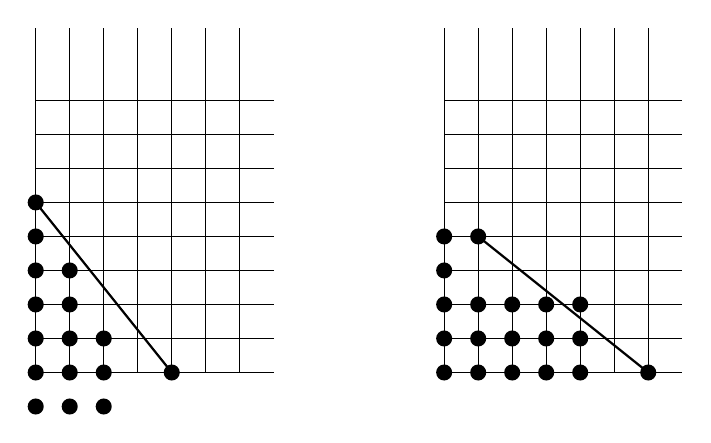
\begin{tikzpicture}[x=1pt,y=1pt,>=stealth,line width=0.5pt]
  \def\u{12.29}
  % ===================== panel a) =====================
  \foreach \i in {0,...,6} {\draw[line width=0.4pt] ({\i*\u},0) -- ({\i*\u},124.4);}
  \foreach \j in {0,...,8} {\draw[line width=0.4pt] (0,{\j*\u}) -- ({7*\u},{\j*\u});}
  \draw[line width=0.8pt] (0,{5*\u}) -- ({4*\u},0);
  \foreach \i/\j in {0/5,0/4,0/3,1/3,0/2,1/2,0/1,1/1,2/1,0/0,1/0,2/0,4/0,0/-1,1/-1,2/-1}
    {\fill ({\i*\u},{\j*\u}) circle[radius=2.9pt];}
  % ===================== panel b) =====================
  \begin{scope}[xshift=147.6pt]
    \foreach \i in {0,...,6} {\draw[line width=0.4pt] ({\i*\u},0) -- ({\i*\u},124.4);}
    \foreach \j in {0,...,8} {\draw[line width=0.4pt] (0,{\j*\u}) -- ({7*\u},{\j*\u});}
    \draw[line width=0.8pt] ({\u},{4*\u}) -- ({6*\u},0);
    \foreach \i/\j in {0/4,1/4,0/3,0/2,1/2,2/2,3/2,4/2,0/1,1/1,2/1,3/1,4/1,0/0,1/0,2/0,3/0,4/0,6/0}
      {\fill ({\i*\u},{\j*\u}) circle[radius=2.9pt];}
  \end{scope}
\end{tikzpicture}

\caption{a）由六维 $A_3$ 理论定义的 Type IV SCFT：非正则奇点的形式由牛顿多边形给出，此外还有一个单正则奇点；图中只写出正则奇点给出的库仑分支参数。b）由 $A_5$ 理论以适当的非正则奇点定义的 Type II SCFT；显式算出谱之后可知，这个理论与 a）等价。}
\label{fig:18}
\end{figure}

再对 $k=2$ 稍作评论：用正则奇点的第一种实现，就是熟悉的 $(A_1,D_{N+2})$ 理论，它由六维 $A_1$ 理论给出。下面说明，这类理论也能只用 $A_N$ 理论的一个非正则奇点实现。

还有更多类似的同构，感兴趣的读者可以自己找一找，这件事颇有乐趣。

\subsubsection{class S 理论的非正则实现}
\label{sec:6.3.1}

\routenote{原文 pp.40--42。这里的路线是把三维镜像反过来用：同一个镜像箭图可以有多种「切成块」的读法，每块读法对应一种奇点结构，于是同一个 class S 理论得到多种非正则实现。作者的检验依据是镜像相同，故库仑分支维数、希格斯分支维数与味对称性都相同。}

还有一类可能的同构，来自对三维镜像对称的考察。最令人惊讶的发现或许是：用带正则穿刺点的球定义的所有理论，都能用非正则奇点实现；而且实现并不唯一。先较仔细地研究带四个味的 $\SU(2)$ 理论，稍后再给一般情形。这个理论有 Gaiotto 找到的六维构造：$A_1$ 理论在球面上放四个正则穿刺点。它的三维镜像很简单，见图 \ref{fig:19}a。

同一个理论有许多非正则实现。先看秩为三的实现：按图 \ref{fig:19}b 的方式看三维镜像。这种看法意味着有一个满正则穿刺点，以及一个带两个满杨图的非正则穿刺点。若按图 \ref{fig:19}c 排布镜像，就得到秩为四的实现：一个分拆为 $[2,2]$ 的正则奇点，加一个带两个满杨图的非正则奇点。秩为五的实现由按图 \ref{fig:19}d 分解镜像得到：只有一个非正则奇点，它有三个杨图，分拆为 $Y_3=[3,2]$、$Y_2=[2,1,1,1]$、$Y_3=[1,1,1,1,1]$。最后还有秩为六的实现：唯一的非正则奇点分拆为 $Y_3=[4,2]$、$Y_2=[2,1,1,1,1]$、$Y_3=[2,1,1,1,1]$，其三维镜像的分解见图 \ref{fig:19}e。
\typo{原文 p.42 在秩 5 与秩 6 的实现中把 $Y_3$ 写了两遍（如 $Y_3=[3,2]$、$Y_2=[2,1,1,1]$、$Y_3=[1,1,1,1,1]$），第三个杨图应为 $Y_1$。译文照录。}

\begin{figure}[tbp]
\centering
% Figure 19 -- a)-e) different decompositions of the 3d mirror of SU(2) with four flavours
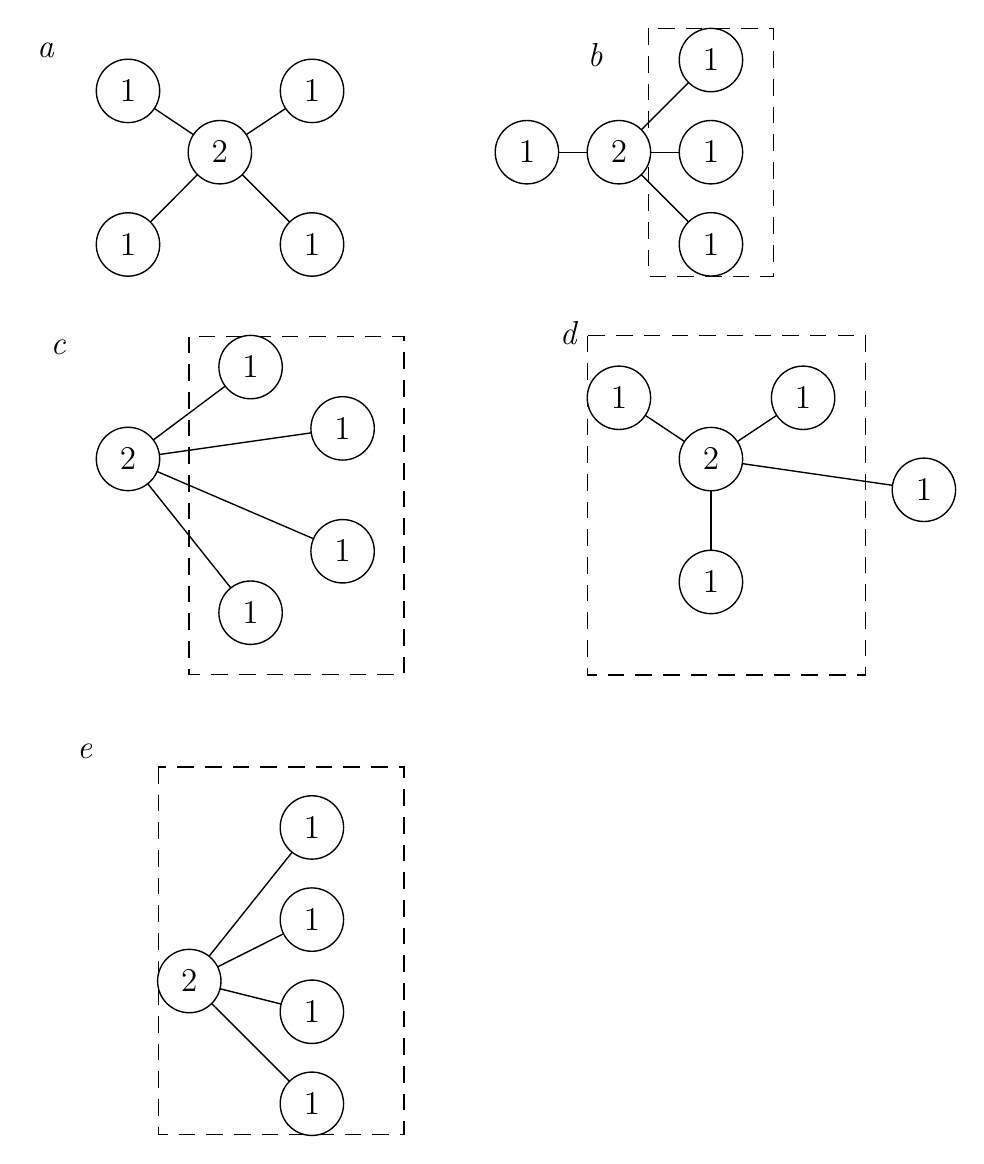
\begin{tikzpicture}[x=1pt,y=1pt,>=stealth,line width=0.5pt,
   nd/.style={circle,draw,fill=white,minimum size=22.9pt,inner sep=0pt,
              font=\fontsize{12}{12}\selectfont},
   bx/.style={draw,line width=0.5pt,dash pattern=on 6pt off 4pt}]
  % ---------------- a) ----------------
  \draw (41.5,381.8) -- (74.7,359.65);
  \draw (41.5,326.3) -- (74.7,359.65);
  \draw (74.7,359.65) -- (108.0,381.8);
  \draw (74.7,359.65) -- (108.0,326.3);
  \node[nd] at (74.7,359.65) {2};
  \node[nd] at (41.5,381.8) {1};
  \node[nd] at (41.5,326.3) {1};
  \node[nd] at (108.0,381.8) {1};
  \node[nd] at (108.0,326.3) {1};
  \node[anchor=base west,font=\fontsize{12.5}{15}\selectfont\itshape] at (5,394) {a};
  % ---------------- b) ----------------
  \draw[bx] (229.6,404.4) rectangle (274.7,314.8);
  \draw (185.65,359.65) -- (218.9,359.65);
  \draw (218.9,359.65) -- (252.15,359.65);
  \draw (218.9,359.65) -- (252.15,392.95);
  \draw (218.9,359.65) -- (252.15,326.35);
  \node[nd] at (185.65,359.65) {1};
  \node[nd] at (218.9,359.65) {2};
  \node[nd] at (252.15,359.65) {1};
  \node[nd] at (252.15,392.95) {1};
  \node[nd] at (252.15,326.35) {1};
  \node[anchor=base west,font=\fontsize{12.5}{15}\selectfont\itshape] at (204,390.5) {b};
  % ---------------- c) ----------------
  \draw[bx] (63.6,293.0) rectangle (141.3,171.0);
  \draw (41.5,248.8) -- (85.8,282.0);
  \draw (41.5,248.8) -- (119.05,259.85);
  \draw (41.5,248.8) -- (119.05,215.45);
  \draw (41.5,248.8) -- (85.8,193.25);
  \node[nd] at (41.5,248.8) {2};
  \node[nd] at (85.8,282.0) {1};
  \node[nd] at (119.05,259.85) {1};
  \node[nd] at (119.05,215.45) {1};
  \node[nd] at (85.8,193.25) {1};
  \node[anchor=base west,font=\fontsize{12.5}{15}\selectfont\itshape] at (10,286.5) {c};
  % ---------------- d) ----------------
  \draw[bx] (207.5,293.4) rectangle (308.0,170.7);
  \draw (252.15,248.75) -- (218.9,270.9);
  \draw (252.15,248.75) -- (285.45,270.9);
  \draw (252.15,248.75) -- (252.15,204.35);
  \draw (252.15,248.75) -- (329.1,237.65);
  \node[nd] at (252.15,248.75) {2};
  \node[nd] at (218.9,270.9) {1};
  \node[nd] at (285.45,270.9) {1};
  \node[nd] at (252.15,204.35) {1};
  \node[nd] at (329.1,237.65) {1};
  \node[anchor=base west,font=\fontsize{12.5}{15}\selectfont\itshape] at (194,290) {d};
  % ---------------- e) ----------------
  \draw[bx] (52.5,137.5) rectangle (141.2,4.8);
  \draw (63.65,60.15) -- (107.95,115.65);
  \draw (63.65,60.15) -- (107.95,82.35);
  \draw (63.65,60.15) -- (107.95,49.05);
  \draw (63.65,60.15) -- (107.95,15.8);
  \node[nd] at (63.65,60.15) {2};
  \node[nd] at (107.95,115.65) {1};
  \node[nd] at (107.95,82.35) {1};
  \node[nd] at (107.95,49.05) {1};
  \node[nd] at (107.95,15.8) {1};
  \node[anchor=base west,font=\fontsize{12.5}{15}\selectfont\itshape] at (19.5,140.5) {e};
\end{tikzpicture}

\caption{带四个味的 $\SU(2)$ 理论的三维镜像的不同分解。每种分解对应一种奇点结构的组合。a）球上有四个正则奇点，每个带一条 $1-2$ 的箭图支链，把各处的 $U(2)$ 味对称性粘合起来即得三维镜像。b）这是秩为三的实现，有一个带箭图支链 $1-2-3$ 的正则奇点，而秩为二的非正则奇点给出一个含三个孤立 $U(1)$ 节点的箭图。于是把正则奇点箭图的 $U(3)$ 节点 spray 成三个 $U(1)$ 节点，再与非正则奇点的箭图粘合。c）这是秩为四的实现，正则奇点的杨图为 $[2,2]$，再加上极点阶为二的非正则奇点，其箭图含四个孤立节点。d）秩为五的实现，只有一个非正则奇点。e）秩为六的实现，只有一个非正则奇点。}
\label{fig:19}
\end{figure}

事实上还有另一种非正则奇点构造，它的三维镜像尚不知道。我们的发现基于线性箭图 $\SU(2)-\SU(4)$，其中 $\SU(4)$ 群并非共形。文献 \cite{32} 指出，其六维构造需要黎曼球上有两个非正则奇点，而 $\SU(2)-4$ 这条支链由如下结构的非正则奇点描述
\begin{equation}
\Phi = z^{-1-\frac{1}{2}}\diag(1,\ w,\ -1,\ -w) ,
\label{eq:6.32}\tag{6.32}
\end{equation}
外加一个 $\SU(4)$ 满正则奇点。我们猜想，这是带四个味的 $\SU(2)$ 理论的另一个秩为四的实现。

把上述做法推广到球面上定义的任何 class S 理论并不难。三维镜像不过是一个星形箭图，它由来自各个穿刺点的箭图支链粘合而成。同一个三维镜像箭图还可以有别的看法，而这些看法都能用非正则奇点实现。不过，不同的实现确实很多。

有几项显式的检验可做：既然三维镜像相同，库仑分支维数与希格斯分支维数就相同，味对称性也相同。这些证据强烈表明：用非正则奇点定义的理论，与球面上带正则奇点定义的 class S 理论是同一个理论。此外，只要取若干有量纲参数之间的比值，就能凑出足够多的无量纲规范耦合常数。我们认为这个值得注意的对偶性很重要，将来还要进一步研究。

\subsection{关于 $R(B)$ 与中心荷 $a$、$c$ 的猜想}
\label{sec:6.4}

中心荷的计算与 $A_1$、$A_2$ 理论的做法很相似：先用镜像对称与算子谱的标度维数算出一部分理论的中心荷，再把结果代入公式 (2.8) 得到函数 $R(B)$。最后用 $R(B)$ 算出这一类中其他理论的中心荷。我们假定 $R(B)$ 有统一的公式，并对 $(A_{k-1},A_{N-1})$ 理论给出显式形式。猜想依据的是下面 $A_1$、$A_2$ 的已知公式，以及 $k$ 与 $N$ 交换下的不变性。我们此前对 $A_1$、$A_2$ 理论的计算给出
\begin{equation}
A_1:\quad R(B) = \frac{1}{2}\,\frac{N(N-1)}{N+2} .
\label{eq:6.33}\tag{6.33}
\end{equation}
\begin{equation}
A_2:\quad R(B) = \frac{3}{2}\,\frac{N(N-1)}{N+3} .
\label{eq:6.34}\tag{6.34}
\end{equation}

我们猜想的普遍公式为
\begin{equation}
A_{k-1}:\quad R(B) = \frac{k(k-1)}{4}\,\frac{N(N-1)}{N+k} ,
\label{eq:6.35}\tag{6.35}
\end{equation}
它在交换 $k$ 与 $N$ 下不变，并能回到 $A_1$、$A_2$ 的情形。

\subsubsection{来自镜像对称的验证}
\label{sec:6.4.1}

可以用三维镜像来检验这个猜想。取三维镜像已知的 $(A_{k-1},A_{nk-1})$ 理论。先用上面猜想的 $R(B)$ 形式算它的中心荷。Seiberg--Witten 曲线为
\begin{equation}
x^k+\bigl(u_1z^{2n-1}+\cdots+u_{2n}\bigr)x^{k-2}
+\bigl(v_1z^{3n-1}+\cdots+v_{3n}\bigr)x^{k-3}
+\cdots+\bigl(z^{nk}+\cdots+c_{nk}\bigr) = 0 ,
\label{eq:6.36}\tag{6.36}
\end{equation}
于是 $z$ 的标度维数为 $[z]=1/(n+1)$。$R(A)$ 可由谱的标度维数求出：
\begin{equation}
R(A) = \sum\bigl(D(u_i)-1\bigr)
= \frac{3kn-3k^2n+kn^2-3k^2n^2+2k^3n^2}{12(1+n)} ,
\label{eq:6.37}\tag{6.37}
\end{equation}
而 $R(B)$ 由我们的拟设给出：
\begin{equation}
R(B) = \frac{k(k-1)}{4}\,\frac{n(nk-1)}{n+1} .
\label{eq:6.38}\tag{6.38}
\end{equation}
利用公式 (2.8)，中心荷为
\begin{equation}
c = \frac{(-1+k)(-2-2n+kn^2+k^2n^2)}{12(1+n)},\qquad
a = \frac{(-1+k)(-5-5n+2kn^2+2k^2n^2)}{24(1+n)} .
\label{eq:6.39}\tag{6.39}
\end{equation}

现在改用另一组方程与三维镜像对称来算。三维镜像理论的库仑分支维数为 $k-1$，因此
\begin{equation}
2a-c = \frac{1}{4}\sum_{i=1}^{r}\bigl(2D(u_i)-1\bigr)
= \frac{3-3k+3n-3kn-kn^2+k^3n^2}{12(1+n)},\qquad
a-c = -\frac{k-1}{24} .
\label{eq:6.40}\tag{6.40}
\end{equation}
我们又得到
\begin{equation}
a = \frac{(-1+k)(-5-5n+2kn^2+2k^2n^2)}{24(1+n)},\qquad
c = \frac{(-1+k)(-2-2n+kn^2+k^2n^2)}{12(1+n)} ,
\label{eq:6.41}\tag{6.41}
\end{equation}
与前面用 $R(B)$ 得到的结果相同。在 $N$ 与 $k$ 都很大的极限下，
\begin{equation}
\frac{a}{c} = 1,\qquad a = \frac{1}{12}k^2N .
\label{eq:6.42}\tag{6.42}
\end{equation}
因此，这一类理论在大 $N$、大 $k$ 极限下有可能找到引力对偶。一旦知道了 $R(B)$，其他三维镜像尚不知道的 $(A_{k-1},A_{N-1})$ 理论的中心荷就容易求出。只要某个子类的三维镜像能找到，同样的方法也可用来算其他类 SCFT 的 $R(B)$。

\subsection{由 $\sN{=}2$ QCD 得到的 AD 点}
\label{sec:6.5}

\routenote{原文 pp.44--46。这里把上一节的做法搬到 $\SU(k)$ QCD：先把 $N_f$ 个味分成两半，各自化成一个非正则奇点，再让两个奇点碰撞。能否碰撞取决于两者的领头阶矩阵是否相同；碰撞后剩下的奇点（可能还带正则奇点）给出 AD 点，属于哪一种由 §6.1 的分类读出。}

我们想找出库仑分支上含有特定 AD 点的线性箭图规范理论。方法是考虑奇点碰撞：两个分数阶奇点若有相同的领头行为，即领头阶矩阵相同，就能相撞。

对带 $N_f$ 个味的 $\SU(k)$ QCD，六维实现并不唯一，而由 $N_f=n_1+n_2$（$n_1\le n_2\le k$）的分拆标记；这基本上是把味分成两组，每组味由一个非正则奇点描述。味数 $l<(k-1)$ 时的非正则奇点为
\begin{equation}
N_f = l:\quad \Phi = \frac{1}{z^{1+1/(k-l)}}\bigl(0,\ \dots,\ 0,\ 1,\ \omega,\ \dots,\ \omega^{k-l-1}\bigr)+\cdots
\label{eq:6.43}\tag{6.43}
\end{equation}
对 $N_f=k-1$，非正则奇点有两个杨图：$Y_2$ 是单杨图，$Y_1$ 是满杨图。对 $N_f=k$，则需要一个满正则奇点与一个单正则奇点。一般说来，只有当味的个数为偶数并等分成两份时才能相撞，但所得的非正则奇点未必定义 AD 理论。按上面 AD 理论的分类与碰撞规则，可在下列情形找到 AD 理论：
\begin{enumerate}[label=\textup{\alph*.}]
  \item 当 $N_f=0$ 时，相撞的非正则奇点具有如下形式
\begin{equation}
\Phi = \frac{1}{z^{2+2/k}}\bigl(1,\ \omega,\ \dots,\ \omega^{k-1}\bigr) .
\label{eq:6.44}\tag{6.44}
\end{equation}
它定义的 AD 理论是 $(A_{k-1},A_1)$ 理论，与文献 \cite{12} 的结果一致。

  \item 当 $N_f=2$ 时，相撞的非正则奇点具有如下形式
\begin{equation}
\Phi = \frac{1}{z^{2+2/(k-1)}}\bigl(0,\ 1,\ \omega,\ \dots,\ \omega^{k-2}\bigr) .
\label{eq:6.45}\tag{6.45}
\end{equation}
借我们发现的同构，它定义的 AD 理论是 $(A_1,D_{k+1})$ 理论，同样与文献 \cite{12} 的结果一致。

  \item 当 $N_f=k$ 且分拆为 $N_f=k\oplus 0$ 时，有一个不描述任何东西的非正则奇点，以及一个满正则奇点与一个单正则奇点。于是可让非正则奇点与满正则奇点相撞，得到如下的合成奇点
\begin{equation}
\Phi = \frac{1}{z^{2+1/k}}\bigl(1,\ \omega,\ \dots,\ \omega^{k-1}\bigr) .
\label{eq:6.46}\tag{6.46}
\end{equation}
此外还有一个单正则奇点，所以碰撞极限下是 type IV SCFT。

  \item 当 $N_f=k+1$ 且分拆为 $N_f=k\oplus 1$ 时，非正则奇点与满正则奇点相撞，产生非正则奇点
\begin{equation}
\Phi = \frac{1}{z^{2+1/(k-1)}}\bigl(0,\ 1,\ \omega,\ \dots,\ \omega^{k-2}\bigr) .
\label{eq:6.47}\tag{6.47}
\end{equation}
这同样是 type IV SCFT，因为还有一个额外的单正则奇点。
\end{enumerate}
一般说来，从 $\SU(k)$ QCD 能找到的 AD 理论就是上面这些。

\subsection{一般的非正则奇点}
\label{sec:6.6}

其余的非正则奇点该作何解释？若领头阶 block 的秩 $r>2$，则 $z$ 具有非平凡的标度维数。我们猜想，其他所有 block 都应当形变到与第一个 block 相同的秩，于是得到一个 AD 理论。因此，若猜想成立，这些一般的非正则奇点确实不必考虑。

若领头阶 block 的秩 $r\le 2$，情形就很不同：此时 $z$ 在旋转下必须平凡地变换，各个 block 地位相同（前面的例子已经用过这一点）。有研究表明，其中一些非正则奇点代表渐近自由理论 \cite{32}。细究这些情形很有意思，留待将来。



% =====================================================================
%  sections/sec7.tex —— 7 已知例子的六维表示（原文 pp.46–48）
% =====================================================================
\section{已知例子的六维表示}
\label{sec:known}

我们已经说明：$(A_1,A_N)$、$(A_1,D_N)$、$(A_1,E_N)$ 理论都可以用六维 $A_1$ 与 $A_2$ 理论配上适当的非正则奇点来工程化。更一般地，$(A_{k-1},A_{N-1})$ 理论也可以用六维 $A_{k-1}$ 或 $A_{N-1}$ 理论来工程化。下面再给一些例子。

$A_0$、$A_1$、$A_2$、$E_6$、$E_7$、$E_8$ 理论都有六维的秩 $N$ 推广（这些名字来自味对称性，以及 Kodaira 对奇异纤维的分类）。秩 $N$ 的 $E_6$、$E_7$、$E_8$ 理论，可以通过把六维 $A_{3N-1}$、$A_{4N-1}$、$A_{6N-1}$ 理论紧致化在只带正则奇点的三孔球上实现 \cite{46}。

现在我们用非正则奇点来工程化秩 $N$ 的 $A_0$、$A_1$、$A_2$ 理论。把 $A_{2N-1}$ 理论紧致化在带下述非正则奇点的球上：
\begin{equation}
A_0:\quad \Phi = \frac{1}{z^{4-1/2}}\diag(\underbrace{1,1,\dots 1}_{N},\ \underbrace{-1,-1,\dots -1}_{N}) + \cdots
\label{eq:7.1}\tag{7.1}
\end{equation}
其领头阶系数有 $N$ 个根 $1$ 与 $N$ 个根 $-1$，次领头阶的项具有同样的模式。这些算子的维数为 $\tfrac{6}{5},\ 2\times\tfrac{6}{5},\ \dots,\ \tfrac{6}{5}N$。

秩 $N$ 的 $A_1$ 理论用 $A_{2N-1}$ 理论与下述非正则奇点来工程化：
\begin{equation}
A_1:\quad \Phi = \frac{1}{z^4}\diag(\underbrace{1,1,\dots 1}_{N},\ \underbrace{-1,-1,\dots -1}_{N}) + \cdots
\label{eq:7.2}\tag{7.2}
\end{equation}
其中 $\tfrac{1}{z^3}\dots\tfrac{1}{z}$ 的系数与领头阶具有同类型的矩阵。谱的标度维数为 $\tfrac{4}{3},\ \tfrac{8}{3},\ \dots,\ \tfrac{4}{3}N$，并且有一个质量参数。

秩 $N$ 的 $A_2$ 理论需要两个奇点：其一为非正则奇点，形式为
\begin{equation}
A_2:\quad \Phi = \frac{1}{z^3}\diag(\underbrace{1,1,\dots 1}_{N},\ \underbrace{-1,-1,\dots -1}_{N}) + \cdots
\label{eq:7.3}\tag{7.3}
\end{equation}
其中 $\tfrac{1}{z^2}\dots\tfrac{1}{z}$ 的系数与领头阶具有同类型的矩阵；其二是一个杨图为 $[N,N]$ 的正则奇点。该理论有 $N$ 个库仑分支算子，维数为 $\tfrac{3}{2},\ \tfrac{3}{2}\times 2,\ \dots,\ \tfrac{3}{2}\times N$，还有两个质量参数。

秩 $N$ 的 $A_1$ 与 $A_2$ 理论的镜像理论画在图 \ref{fig:20} 中。利用谱的信息与镜像对称，可以算出中心荷 $a$ 与 $c$。对秩 $N$ 的 $A_1$ 理论，镜像的库仑分支维数为 $2N-1$，于是
\begin{equation}
2a-c = \frac{1}{4}\sum_i\bigl(2D(u_i)-1\bigr) = \frac{1}{12}(N+4N^2),\qquad
a-c = -\frac{2N-1}{24},
\label{eq:7.4}\tag{7.4}
\end{equation}
从而
\begin{equation}
a = \frac{1}{24}(-1+4N+8N^2),\qquad c = \frac{1}{12}(-1+3N+4N^2).
\label{eq:7.5}\tag{7.5}
\end{equation}
类似地，对秩 $N$ 的 $A_2$ 理论，镜像的库仑分支维数为 $3N-1$，于是
\begin{equation}
2a-c = \frac{1}{8}(N+3N^2),\qquad a-c = -\frac{3N-1}{24},
\label{eq:7.6}\tag{7.6}
\end{equation}
从而
\begin{equation}
a = \frac{1}{24}(-1+6N+9N^2),\qquad c = \frac{1}{24}(-2+9N+9N^2).
\label{eq:7.7}\tag{7.7}
\end{equation}
这些结果与 \cite{21} 一致。

文献 \cite{47,48} 用奇点理论找到的一些 SCFT，同样可以用非正则奇点来工程化。只举一个例子：所谓的 W13 理论，它在奇点处的 Seiberg--Witten 曲线为
\begin{equation}
x^4 + x y^4 = 0 .
\label{eq:7.8}\tag{7.8}
\end{equation}
显然，这就是用六维 $A_3$ 理论构造的 type II SCFT。

\begin{figure}[tbp]
\centering
% Figure 20 -- (a) 3d mirror for rank N A_1 theory, (b) for rank N A_2 theory
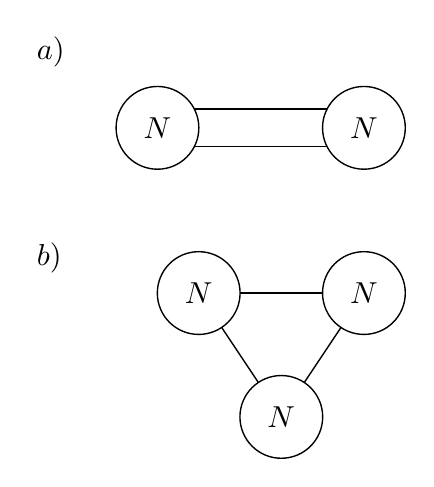
\begin{tikzpicture}[x=1pt,y=1pt,>=stealth,line width=0.5pt,
   nd/.style={circle,draw,fill=white,minimum size=29.9pt,inner sep=0pt,
              font=\fontsize{11}{11}\selectfont}]
  % ---------------- a) ----------------
  \draw (59.15,140.1) -- (133.75,140.1);
  \draw (59.15,126.6) -- (133.75,126.6);
  \node[nd] at (59.15,133.35) {$N$};
  \node[nd] at (133.75,133.35) {$N$};
  \node[anchor=base west,font=\fontsize{10.7}{10.7}\selectfont] at (12,158) {$a)$};
  % ---------------- b) ----------------
  \draw (74.05,73.65) -- (133.75,73.65);
  \draw (74.05,73.65) -- (103.9,28.9);
  \draw (133.75,73.65) -- (103.9,28.9);
  \node[nd] at (74.05,73.65) {$N$};
  \node[nd] at (133.75,73.65) {$N$};
  \node[nd] at (103.9,28.9) {$N$};
  \node[anchor=base west,font=\fontsize{10.7}{10.7}\selectfont] at (12,83.5) {$b)$};
\end{tikzpicture}

\caption{(a) 秩 $N$ 的 $A_1$ 理论的三维镜像。(b) 秩 $N$ 的 $A_2$ 理论的三维镜像。}
\label{fig:20}
\end{figure}


% =====================================================================
%  sections/sec8.tex —— 8 结论 + 致谢（原文 pp.48–50）
% =====================================================================
\section{结论}
\label{sec:concl}

本文用六维构造造出了一大类 AD 型理论。我们求出了 Seiberg--Witten 曲线与谱的标度维数，还借助三维镜像对称算出了中心荷 $a$ 与 $c$。我们也识别出了 $\SU(N)$ QCD 的 AD 点。

最初，有拉氏量描述的 $\sN{=}2$ SCFT 由 ADE Dynkin 图分类 \cite{49}。Gaiotto 用黎曼面上的正则穿刺点找到了一大类新的 SCFT \cite{2}，而这些理论一般没有拉氏量描述。在球面的情形，它们就是带强耦合物质系统的 $A_n$ 型广义箭图规范理论。这些结果极大地增加了 $\sN{=}2$ SCFT 的数目。上述理论都只有整数标度维数与无量纲的耦合常数。通过允许分数标度维数，我们说明了 $\sN{=}2$ SCFT 的版图被极大扩展，而且实际上把此前构造的那些理论（至少是定义在球面上的那些）作为一个很小的角落包含进来。考虑到 SCFT 的重要性，如此大量的例子应当对我们认识量子场论的动力学非常有帮助。

AD 理论虽然在 1995 年就被发现了，但人们对它们的性质了解甚少，相关研究也不多。有了六维构造，我们相信现在可以更细致地理解这些理论。大体上说，凡是针对 class S 理论做过的事情，稍加努力都可以推广到这些 AD 理论上。下面列出一些有意思的问题：

\begin{enumerate}[label=\textup{\alph*.}]
  \item 本文只考虑了六维 $A_n$ 理论，推广到六维 $D_n$ 与 $E_n$ 理论应当是直接的。文献 \cite{28} 研究了一般约化群的非正则奇点与广义单值性，可以利用这些结果构造新类型的 Argyres--Douglas 理论。
  \item 四维 $\sN{=}2$ 理论引力对偶的一般拟设已在 \cite{50} 中写出，而引力解归结为求解三维 Toda 方程。正则奇点的情形已在 \cite{51} 中研究过。通过研究 Toda 方程的非正则解，应当能够找到本文所构造 AD 理论的引力对偶。由于定义在球面上的 class S 理论也有非正则奇点的表示，利用非正则奇点或许更容易得到引力对偶。高秩 $(A_0,A_1,A_2)$ AD 理论的引力对偶已在 \cite{52} 中用 F 理论找到。既然我们给出了显式的六维构造，上述结果也许有助于求出一般的解。
  \item 只由正则穿刺点定义的场论，其丛坐标已在 \cite{53} 中构造出来。那套构造同样适用于本文构造的 AD 理论。思路是这样的：非正则奇点造出一个带多个标记点的边界，因此几何其实是带标记点的圆盘，\cite{53} 的构造很容易搬过来。问题就归结为：对某个特定的非正则奇点，要确定边界上有多少个标记点、以及该放什么杨图 \cite{30}。一旦求出丛坐标，就可以用它们研究线算子的分类、BPS 谱与墙穿越、面算子等等。
  \item $A_1$ AD 理论的 AGT 猜想 \cite{54} 已在 \cite{55,56} 中研究过，其中牵涉 Liouville 理论的非正则共形块。把这个猜想推广到本文构造的更高秩 AD 理论应当是可以做到的。由于这些理论没有拉氏量，必须另想办法求 Nekrasov 配分函数；在存在非正则奇点时，只要我们对平坦联络的模空间有好的坐标，\cite{57} 所述的方法应当有用。由 $A_1$ 理论构造的渐近自由理论的 AGT 猜想也已有研究 \cite{58}，把那一构造推广到本文构造的所有渐近自由理论同样有意思。
  \item Seiberg--Witten 解定义一个可积系统，而四维 $\sN{=}2$ 理论的配分函数与可积系统的 Yang--Yang 函数之间的 Nekrasov--Shatashvili 关系，在这里也可以推广。看起来，只要丛坐标已知，\cite{59} 构造的 Darboux 坐标就可以推广到我们的情形。事实上，在正则穿刺点的情形，他们用的是裤分解中的那些圈，而这些圈实际上标定了 Teichmüller 空间的叶层化空间。把叶层化推广到圆盘的做法见 \cite{60}；只要知道丛坐标，就应当能够写出 Darboux 坐标对应表达式的描述。
  \item 数学上，非正则奇点与可积系统近年来已被大量研究 \cite{61}，我们预期这些结果对计算 AD 理论的共形块有用。我们已经说明，同一个理论既可以用正则奇点、也可以用非正则奇点来实现；这一事实对研究几何 Langlands 纲领中的驯顺分歧与野分歧是否有用？此外，两种实现对应的等单值形变方程已被证明是等价的 \cite{62}，看看这对相应的场论意味着什么是很有意思的。
  \item 一旦知道这些更高秩 AD 理论的 BPS 谱，就可以沿 \cite{63} 中发展出的路子研究更高秩的三维四面体理论与相应的 $\sN{=}2$ 理论。例如，更高秩五边形理论的 BPS 谱似乎比较容易算（$A_2$ 实现的 $E_7$ 理论边界上有五个标记点）。
  \item 我们已经算出了一些 AD 理论的中心荷 $a$ 与 $c$。在这些理论之间找出重整化群流并不困难，显式检验 $a$ 定理应当很有意思。四维 $a$ 定理的一般证明在 \cite{64} 中讨论过；若能构造许多显式例子，对理解那个证明应当有帮助。
  \item 对每个 AD 理论，它的丛坐标对应于圆盘上的一个平面二部图。这类平面二部图在研究 $\sN{=}4$ 超杨–米尔斯理论的散射振幅时被大量使用 \cite{65}。同一个数学结构出现在两个看来完全不同的物理系统中，弄清这里是否有更深层的联系很有意思。AD 理论的物理可观测量与 $\sN{=}4$ 超杨–米尔斯的散射振幅会有关系吗？此外，平面二部图已在 \cite{66} 中被完全分类，能否用这个结果给 AD 理论一个另外的分类？
  \item 还有一些别的物理量是人们想算的。例如：算出 type IV AD 理论的中心荷 $k$ 会很有意思，它衡量非阿贝尔味对称性被规范之后对 $\beta$ 函数的贡献。算这些理论的超共形指标也有意思，正则穿刺点情形的结果见 \cite{67}。我们还想更细致地研究 AD 理论的希格斯分支，它似乎可以由三维镜像理论的库仑分支来捕捉，如此等等。
\end{enumerate}

\typo{第 (d) 条里的「AGT 猜想」在原文 p.49 有一处印作 "ACT conjecture"（同一条前面写的是 AGT），应为 AGT。第 (j) 条原文用 $k$ 表示这个中心荷，与全文用 $k$ 表示 block 大小、规范群秩的用法冲突；译文照录。}

\section*{致谢}
\addcontentsline{toc}{section}{致谢}

感谢 Nima Arkani-Hamed、Davide Gaiotto、Yu-tin Huang、Hai Lin、Juan Maldacena、Andrew Neitzke、Edward Witten、Yuji Tachikawa、Peng Zhao 的有益讨论。DX 的研究受 Zurich Financial Services 的会员资格资助，并感谢美国能源部 grant DE-FG02-90ER40542 的支持。


% ---------------------------- 参考文献 ----------------------------
% =====================================================================
%  refs.tex —— 参考文献（原文 pp.50–54）。条目按底本原样保留英文。
% =====================================================================
\addcontentsline{toc}{section}{参考文献}
\begin{thebibliography}{99}
\bibitem{1} E. Witten, “Geometric Langlands from six dimensions,” arXiv:0905.2720 [hep-th].
\bibitem{2} D. Gaiotto, “N = 2 dualities,” arXiv:0904.2715 [hep-th].
\bibitem{3} D. Gaiotto, G. W. Moore, and A. Neitzke, “Wall-crossing, hitchin Systems, and the WKB approximation,” arXiv:0907.3987 [hep-th].
\bibitem{4} P. C. Argyres and N. Seiberg, “S-Duality in N = 2 supersymmetric gauge theories,” JHEP 12 (2007) 088, arXiv:0711.0054 [hep-th].
\bibitem{5} J. A. Minahan and D. Nemeschansky, “An N = 2 superconformal fixed point with E6 global symmetry,” Nucl. Phys. B482 (1996) 142–152, arXiv:hep-th/9608047.
\bibitem{6} P. C. Argyres and M. R. Douglas, “New phenomena in SU(3) supersymmetric gauge theory,” Nucl.Phys. B448 (1995) 93–126, arXiv:hep-th/9505062 [hep-th].
\bibitem{7} P. C. Argyres, M. Plesser, and A. D. Shapere, “The Coulomb phase of N=2 supersymmetric QCD,” Phys.Rev.Lett. 75 (1995) 1699–1702, arXiv:hep-th/9505100 [hep-th].
\bibitem{8} N. Hitchin, “The self-duality equation on a riemann surface,” Proc.London Math.Soc. (3)55 (1987) 59–126.
\bibitem{9} N. Hitchin, “Stable bundles and integrable system,” Duke Math. J. (1)54 (1987) 91–114.
\bibitem{10} O. Biquard and P. Boalch, “Wild non-abelian Hodge theory on curves,” Compos. Math. 140 (2004) no. 1, 179–204. http://dx.doi.org/10.1112/S0010437X03000010.
\bibitem{11} P. C. Argyres, M. Ronen Plesser, N. Seiberg, and E. Witten, “New N=2 superconformal field theories in four-dimensions,” Nucl.Phys. B461 (1996) 71–84, arXiv:hep-th/9511154 [hep-th].
\bibitem{12} T. Eguchi, K. Hori, K. Ito, and S.-K. Yang, “Study of N = 2 Superconformal Field Theories in 4 Dimensions,” Nucl. Phys. B471 (1996) 430–444, arXiv:hep-th/9603002.
\bibitem{13} T. Eguchi and K. Hori, “N = 2 superconformal field theories in 4 dimensions and A- D-E classification,” arXiv:hep-th/9607125.
\bibitem{14} T. Banks, M. R. Douglas, and N. Seiberg, “Probing F-theory with branes,” Phys. Lett. B387 (1996) 278–281, arXiv:hep-th/9605199.
\bibitem{15} M. R. Douglas, D. A. Lowe, and J. H. Schwarz, “Probing F-theory with multiple branes,” Phys. Lett. B394 (1997) 297–301, arXiv:hep-th/9612062.
\bibitem{16} S. Gukov and A. Kapustin, “New N = 2 superconformal field theories from M/F theory orbifolds,” Nucl. Phys. B545 (1999) 283–308, arXiv:hep-th/9808175.
\bibitem{17} S. Cecotti, A. Neitzke, and C. Vafa, “R-twisting and 4d/2d correspondences,” arXiv:1006.3435 [hep-th].
\bibitem{18} J. Seo and K. Dasgupta, “Argyres-Douglas Loci, Singularity Structures and Wall- Crossings in Pure N=2 Gauge Theories with Classical Gauge Groups,” arXiv:1203.6357 [hep-th].
\bibitem{19} S. M. Kuzenko and S. Theisen, “Correlation functions of conserved currents in N = 2 superconformal theory,” Class. Quant. Grav. 17 (2000) 665–696, arXiv:hep-th/9907107.
\bibitem{20} A. D. Shapere and Y. Tachikawa, “Central charges of N=2 superconformal field theories in four dimensions,” JHEP 0809 (2008) 109, arXiv:0804.1957 [hep-th].
\bibitem{21} O. Aharony and Y. Tachikawa, “A holographic computation of the central charges of d=4, N=2 SCFTs,” JHEP 01 (2008) 037, arXiv:0711.4532 [hep-th].
\bibitem{22} D. Gaiotto, N. Seiberg, and Y. Tachikawa, “Comments on scaling limits of 4d N=2 theories,” JHEP 01 (2011) 078, arXiv:1011.4568 [hep-th].
\bibitem{23} D. Nanopoulos and D. Xie, “Hitchin equation, singularity, and N = 2 superconformal field theories,” JHEP 03 (2010) 043, arXiv:0911.1990 [hep-th].
\bibitem{24} A. Kapustin, “Solution of N = 2 gauge theories via compactification to three dimensions,” Nucl. Phys. B534 (1998) 531–545, arXiv:hep-th/9804069.
\bibitem{25} A. Kapustin and E. Witten, “Electric-Magnetic duality and the Geometric Langlands Program,” arXiv:hep-th/0604151.
\bibitem{26} E. Witten, “Gauge theory and wild ramification,” arXiv:0710.0631 [hep-th].
\bibitem{27} W. Wasow, Asymptotic expansions for ordinary differential equations. Dover Publications Inc., New York, 1987. Reprint of the 1976 edition.
\bibitem{28} P. P. Boalch, “G-bundles, isomonodromy, and quantum Weyl groups,” Int. Math. Res. Not. (2002) no. 22, 1129–1166. http://dx.doi.org/10.1155/S1073792802111081.
\bibitem{29} S. Gukov and E. Witten, “Gauge Theory, ramification, and the Geometric Langlands Program,” arXiv:hep-th/0612073.
\bibitem{30} D. Xie, “Network, cluster coordinates and N = 2 theory II: Irregular singularity,” arXiv:1207.6112 [hep-th].
\bibitem{31} S. Cecotti and C. Vafa, “Classification of complete N=2 supersymmetric theories in 4 dimensions,” arXiv:1103.5832 [hep-th].
\bibitem{32} D. Nanopoulos and D. Xie, “Hitchin equation, irregular Singularity, and N = 2 asymptotical free theories,” arXiv:1005.1350 [hep-th].
\bibitem{33} A. D. Shapere and C. Vafa, “BPS structure of Argyres-Douglas superconformal theories,” arXiv:hep-th/9910182.
\bibitem{34} M. Alim, S. Cecotti, C. Cordova, S. Espahbodi, A. Rastogi, and C. Vafa, “BPS Quivers and Spectra of Complete N=2 Quantum Field Theories,” arXiv:1109.4941 [hep-th].
\bibitem{35} M. Alim, S. Cecotti, C. Cordova, S. Espahbodi, A. Rastogi, and C. Vafa, “N=2 Quantum Field Theories and Their BPS Quivers,” arXiv:1112.3984 [hep-th].
\bibitem{36} D. Gaiotto, G. W. Moore, and A. Neitzke, “Framed BPS states,” arXiv:1006.0146 [hep-th].
\bibitem{37} D. Gaiotto, G. W. Moore, and A. Neitzke, “Wall-Crossing in Coupled 2d-4d Systems,” arXiv:1103.2598 [hep-th].
\bibitem{38} F. Benini, Y. Tachikawa, and D. Xie, “Mirrors of 3d Sicilian theories,” JHEP 1009 (2010) 063, arXiv:1007.0992 [hep-th].
\bibitem{39} P. Boalch, “Irregular connections and Kac-Moody root systems,” arXiv:0806.1050.
\bibitem{40} D. Nanopoulos and D. Xie, “More three dimensional mirror pairs,” arXiv:1011.1911 [hep-th].
\bibitem{41} S. A. Cherkis and A. Kapustin, “Periodic monopoles with singularities and N = 2 super-QCD,” Commun. Math. Phys. 234 (2003) 1–35, arXiv:hep-th/0011081.
\bibitem{42} D. Gaiotto, “unpublished,”.
\bibitem{43} S. Fomin, M. Shapiro, and D. Thurston, “Cluster algebras and triangulated surfaces. part i: Cluster complexes,” ACTA MATHEMATICA 201 (2008) 83. arXiv.org:math/0608367.
\bibitem{44} K. A. Intriligator and N. Seiberg, “Mirror symmetry in three dimensional gauge theories,” Phys. Lett. B387 (1996) 513–519, arXiv:hep-th/9607207.
\bibitem{45} E. Witten, “Solutions of four-dimensional field theories via M-theory,” Nucl. Phys. B500 (1997) 3–42, arXiv:hep-th/9703166.
\bibitem{46} F. Benini, S. Benvenuti, and Y. Tachikawa, “Webs of five-Branes and N = 2 superconformal field theories,” JHEP 09 (2009) 052, arXiv:0906.0359 [hep-th].
\bibitem{47} S. Cecotti and M. Del Zotto, “On Arnold’s 14 ‘exceptional’ N=2 superconformal gauge theories,” JHEP 10 (2011) 099, arXiv:1107.5747 [hep-th].
\bibitem{48} M. Del Zotto, “More Arnold’s N = 2 superconformal gauge theories,” JHEP 11 (2011) 115, arXiv:1110.3826 [hep-th].
\bibitem{49} S. Katz, P. Mayr, and C. Vafa, “Mirror symmetry and exact solution of 4D N = 2 gauge theories. I,” Adv. Theor. Math. Phys. 1 (1998) 53–114, arXiv:hep-th/9706110.
\bibitem{50} H. Lin, O. Lunin, and J. M. Maldacena, “Bubbling AdS space and 1/2 BPS geometries,” JHEP 10 (2004) 025, arXiv:hep-th/0409174.
\bibitem{51} D. Gaiotto and J. Maldacena, “The gravity duals of N = 2 superconformal field theories,” arXiv:0904.4466 [hep-th].
\bibitem{52} O. Aharony, A. Fayyazuddin, and J. M. Maldacena, “The large N limit of N = 2,1 field theories from three- branes in F-theory,” JHEP 07 (1998) 013, arXiv:hep-th/9806159.
\bibitem{53} D. Xie, “Network, Cluster coordinates and N=2 theory I,” arXiv:1203.4573 [hep-th].
\bibitem{54} L. F. Alday, D. Gaiotto, and Y. Tachikawa, “Liouville correlation functions from four-dimensional gauge theories,” Lett. Math. Phys. 91 (2010) 167–197, arXiv:0906.3219 [hep-th].
\bibitem{55} D. Gaiotto and J. Teschner, “Irregular singularities in Liouville theory,” arXiv:1203.1052 [hep-th].
\bibitem{56} G. Bonelli, K. Maruyoshi, and A. Tanzini, “Wild Quiver Gauge Theories,” JHEP 02 (2012) 031, arXiv:1112.1691 [hep-th].
\bibitem{57} N. Nekrasov and E. Witten, “The Omega deformation, branes, integrability, and liouville Theory,” JHEP 09 (2010) 092, arXiv:1002.0888 [hep-th].
\bibitem{58} D. Gaiotto, “Asymptotically free N=2 theories and irregular conformal blocks,” arXiv:0908.0307 [hep-th].
\bibitem{59} N. Nekrasov, A. Rosly, and S. Shatashvili, “Darboux coordinates, Yang-Yang functional, and gauge theory,” Nucl. Phys. Proc. Suppl. 216 (2011) 69–93, arXiv:1103.3919 [hep-th].
\bibitem{60} V. V. Fock and A. B. Goncharov, “The quantum dilogarithm and representations quantum cluster varieties,” arXiv:0702397 [math].
\bibitem{61} B. Feigin, E. Frenkel, and V. Toledano-Laredo, “Gaudin models with irregular singularities,” 2006. doi:10.1016/j.aim.2009.09.007.
\bibitem{62} P. Boalch, “Simply-laced isomonodromy systems,” 2011. http://www.citebase.org/abstract?id=oai:arXiv.org:1107.0874.
\bibitem{63} S. Cecotti, C. Cordova, and C. Vafa, “Braids, Walls, and Mirrors,” arXiv:1110.2115 [hep-th].
\bibitem{64} Z. Komargodski and A. Schwimmer, “On Renormalization Group Flows in Four Dimensions,” JHEP 12 (2011) 099, arXiv:1107.3987 [hep-th].
\bibitem{65} N. Arkani-Hamed, J. L. Bourjaily, F. Cachazo, A. B. Goncharov, A. Postnikov, and J. Trnka, Scattering Amplitudes and the Positive Grassmannian. Cambridge University Press, 2012. arXiv:1212.5605 [hep-th]. http://inspirehep.net/record/1208741/files/arXiv:1212.5605.pdf.
\bibitem{66} A. Postnikov, “Total positivity, grassmannians, and networks,”. arXiv.org:math/0609764.
\bibitem{67} A. Gadde, L. Rastelli, S. S. Razamat, and W. Yan, “Gauge Theories and Macdonald Polynomials,” arXiv:1110.3740 [hep-th].
\end{thebibliography}


\end{document}
